\documentclass{izdthesis}

\usepackage{float}
\usepackage{longtable} % 表 5.1 单元测试表内容较多，需跨页排版

% 4.4.2 节下含四级标题（4.4.2.1 等），需对 subsubsection 编号（不进目录）
\setcounter{secnumdepth}{3}
\ctexset{
  subsubsection = {
    format      = \zihao{-4}\heiti,
    aftername   = \hspace{0.5em},
    beforeskip  = 0.5\baselineskip,
    afterskip   = 0.5\baselineskip,
  },
}

\ctitle{基于SpringCloud的企业系统自动生成平台}
\etitle{SpringCloud-Based Enterprise System Automatic Generation Platform}
\stuname{曹剑澄}
\college{软件与通信学院}
\major{软件工程}
\advisor{张磊}
\advisortitle{副教授}
\finishdate{2021 年 6 月}
\gradyear{2021}

\begin{document}

\makecover

\makedeclaration

\begin{cnabstract}
随着软件技术与人们的生活日益密切，各行各业对管理系统的依赖也越来越深。因此软件公司在接到客户需求后，如何能够根据需求高效、稳定的完成相应系统设计与开发工作，成为各软件公司研究的重点方向。在这种市场环境下，代码生成技术飞速发展，与此同时，也面临着很多问题。其中生成代码混乱、难以使用与维护，是重点问题。开发人员面对生成的代码不能够快速了解其结构并进行使用，在浪费时间的同时还可能会留下隐患，没有达到使用代码生成系统进行开发的根本要求。因此，本人调研了软件系统的编码规范、系统安全、用户需求等，开发基于 SpringCloud 的企业系统自动生成平台，能够实现快速开发、0 代码系统搭建、规范化生成代码等，解决上述问题。

通过对调研结果及多家企业客户的需求分析，在此基础上根据需求确定平台设计原则，实现了平台整体结构的设计和功能的划分，完成了项目设计并绘制了系统用例图等。该平台通过 Velocity 生成后台代码，Velocity 是基于 Java 的代码生成器，它在简单、规范的同时还具有良好的性能。平台的前端采用 FG（Form Generator）和 JB(JeecgBoot) 表单设计及代码生成器，通过 Online 代码生成使用户根据需求对页面进行个性化设计。该代码生成器能够在线配置数据库和页面控件，并可进行实时预览，可根据用户配置的表单结构自动选择相应的代码生成器模板。对于后端代码生成这部分功能，平台采用了阿里巴巴的《Java 开发手册》作为编码规范；而前端采用的是通用编码规范，尽可能地使代码更易于维护和理解。平台基于微服务架构（SpringCloud）研发，使用此架构使每个服务内部高内聚，服务之间低耦合，代码可读性更高，大大提高了开发效率；由于该平台每个服务可单独部署在不同的服务器上，所以平台具有良好的可扩展性和较高的容错性。除此之外，平台还包括完备的登录、用户管理、角色管理、系统日志等基础功能。

通过测试，基于本平台生成的代码包含代码注解，可帮助开发人员快速了解核心代码含义。所有代码均按照统一编码规范开发，成功实现了简洁方便、代码规范化、易用性与可维护性高的目标。本平台可以为开发者提供一个具有高自由度、高跨平台性、操作简单、可自主配置并具有标准代码规范的代码生成系统。目前本平台应用于国内多家软件公司，得到了用户们的一致好评。

\keywords{代码生成；SpringCloud；企业系统；自动化；跨平台；高扩展性}
\end{cnabstract}

\begin{enabstract}
As software technology becomes closer to people's lives, all walks of life are becoming more and more dependent on management systems. Therefore, how software companies can complete the corresponding system design and development work efficiently and stably after receiving customer needs has become the key research direction of software companies. In this market environment, code generation technology is developing rapidly, and at the same time, it is also facing many problems. Among them, the generated code is messy, difficult to use and maintain, which are key issues. In the face of the generated code, developers cannot quickly understand its structure and use it. While wasting time, they may also leave hidden dangers, failing to meet the fundamental requirements of using a code generation system for development. Therefore, I investigated the coding specifications, system security, user needs, etc. of the software system, and developed an automatic generation platform for enterprise systems based on SpringCloud, which can achieve rapid development, zero-code system construction, standardized code generation, etc., to solve the above problems. Through the analysis of the survey results and the needs of many corporate customers, on this basis, the platform design principles were determined according to the needs, the overall structure of the platform and the division of functions were realized, the project design was completed and the system use case diagram was drawn. The platform generates back-end code through Velocity. Velocity is a Java-based code generator, which is simple, standardized, and has good performance. The front end of the platform adopts FG (Form Generator) and JB (JeecgBoot) form design and code generators, and online code generation enables users to personalize the page design according to their needs. The code generator can configure the database and page controls online, and can perform real-time preview, and can automatically select the corresponding code generator template according to the form structure configured by the user. For the back-end code generation function, the platform uses Alibaba's "Java Development Manual" as the coding specification; while the front-end uses a general coding specification to make the code easier to maintain and understand as much as possible. The platform is developed based on the microservice architecture (SpringCloud). Using this architecture enables high internal cohesion of each service, low coupling between services, higher code readability, and greatly improved development efficiency; because each service of the platform can be deployed separately on different servers, the platform has good scalability and high fault tolerance. In addition, the platform also includes complete basic functions such as login, user management, role management, and system logs. Through testing, the code generated based on this platform contains code annotations, which can help developers quickly understand the meaning of the core code. All codes are developed in accordance with the unified coding standard, which has successfully achieved the goals of simplicity and convenience, standardization of the code, high ease of use and maintainability. This platform can provide developers with a code generation system with high degree of freedom, high cross-platform, simple operation, independent configuration, and standard code specifications. At present, this platform is used in many domestic software companies and has been well received by users.

\enkeywords{Code Generation；SpringCloud；Enterprise System；Automation；Cross-platform；High scalability}
\end{enabstract}

\izdtableofcontents

\izdmainmatter

\chapter{引言}

\section{研究背景}
随着互联网的高速发展，软件产品已经成为了人们生活中不可分割的一部分，人们无时无刻不在享受着网络所带来的便利。在国民经济的建设中，软件也发挥着越来越重要的作用。各行各业越来越多地使用软件系统进行工作、管理，既能简化工作流程、提高工作效率，又能满足各行业的管理需求。因此，市场上对软件系统的需求量增大，面对软件系统的技术也飞速发展。

Java EE 架构分层体系结构在软件开发中体现了独特的好处，很大程度上解决了系统的耦合性过高的问题，增强了系统可维护性。但是耦合度降低的同时也存在代码量急剧增加的问题\cite{ref1}，而传统代码开发成本随着市场需求的增长越来越高，尤其是人力成本的不断升高，普通软件产品的功能已经无法满足企业的管理需求，客户对产品的要求逐渐向着功能多样化、操作简单化发展。为了节约成本、提高开发效率、增强软件质量，许多软件公司将底层代码封装起来，形成一定的开发模式以帮助开发人员简化开发，例如 Spring MVC、SpringBoot、Hibernate 等框架应运而生。这些框架通过对底层原生代码的封装映射，使开发者能有更多的时间完成功能，而不是花费时间成本去关注底层代码。

但从目前的市场需求来看，单纯的系统框架已经不能满足越来越复杂的开发过程，软件开发又面临着新的挑战：
\begin{itemize}
  \item 项目需求集中出现\par
  受各行各业的实际情况影响，会导致在某一时间段内出现大量项目，但软件公司的人力资源有限，不可能同时接收大量项目，这就直接影响了公司的收益。
  \item 项目难以维护\par
  每个开发者都有自己的编码风格，因此产品交付时系统的代码风格迥异，给后期的扩展、维护带来了很大困难。
  \item 项目质量难以保证\par
  每个项目都有着严格的交付验收时间，在时间紧迫、工作压力大的情况下，项目质量就很难得到保证，甚至可能会出现项目延期、客户满意度降低等后果。
  \item 大量重复工作\par
  在项目开发过程中，各功能模块的基础功能都是一样的，尤其是大型系统中动辄使用几十个功能模块。开发者们在编写基础的、大量重复的代码上需要花费大量时间，这使得项目的时间成本进一步提高。
  \item 个性化样式\par
  客户在要求功能的同时，更希望能有一个美观、标准、展现自己风格的系统样式，而在开发过程中调整前端样式同样是一项复杂、细致、占用大量时间的工作。
\end{itemize}

综上所述，目前市场需要一种新的开发模式来帮助开发人员更加便捷高效地完成开发工作。这种模式要具有高效性，并且能够快速完成项目基础环境的搭建，缩短项目开发周期；要具有统一的编码格式，使开发者更易于理解，为后期项目扩展和维护提供便利；能帮助开发者减少繁多的基础代码和统一标准样式所带来的工作量，减轻开发人员的负担\cite{ref2}。

基于 Java 的 Online 代码生成器（JEECG）的功能和前端组件，实现了通过数据库结构快速生成相应基础 CURD（Create、Update、Read、Delete）代码，并可根据不同的项目需求选择所需配置文件，最终实现项目基础框架和基础代码的快速开发。这一方式大幅度缩短了项目从完成设计到实现的时间，生成的代码具有统一的编码风格并使开发人员避免了重复代码的编写，极大地降低了时间成本和人力成本。前端页面通过拖拽的方式可快速搭建所需页面，自定义页面样式，最大限度地解决了调整样式的复杂工作，帮助开发人员摆脱琐碎的工作，能有更多的时间完成逻辑的编写和系统性能的优化\cite{ref3}。

\section{国内外研究现状}
代码自动生成技术原本是应用于各种代码的编译器中，编译器通过代码生成器将高级语言编译成汇编语言及机器语言。在本文中所描述的代码生成平台中，代码生成并不是编译器中的生成技术，而是一种软件工程技术。它通过使用代码编译器根据一定的规则（特定的文本或代码等），自动生成 Java、Vue、XML 等高级编程语言。

\subsection{国外研究状况}
代码自动生成技术的研究从 1992 年出现，到 2012 年达到高潮，到 2016 年为止已有 443 篇相关研究论文（数据来源于百度学术，截止日期为 2020 年 11 月 7 日）。如图 \ref{fig1-1} 所示。

\begin{figure}[H]
  \centering
  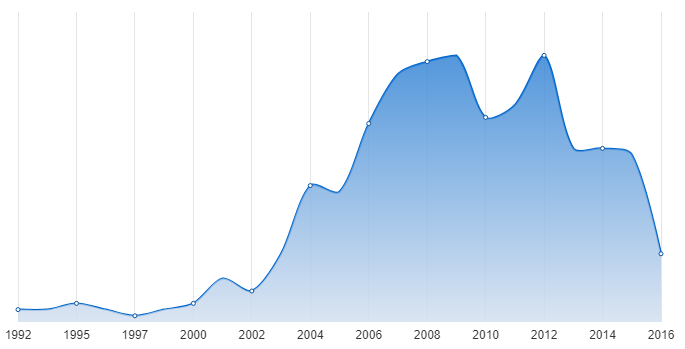
\includegraphics[width=0.7\textwidth]{figures/fig1-1.png}
  \caption{代码自动生成技术研究走势图}
  \label{fig1-1}
\end{figure}

经过长时间的发展和不断的演化，现在的代码生成技术已经得到了长足的发展，出现了各种各样的代码生成器，其中大多数是基于模型架构或是模型驱动架构的代码生成工具。现在国外的许多一线互联网公司都在进行有关工具或架构的研究。有的公司通过构建的系统模型来自动生成代码，譬如 Rational 公司的 Rational Rose\cite{ref4}，通过用户创建的模型和语言类型自动生成相应代码。有的公司利用创建好的数据库结构或者数据源进行代码生成，例如，微软的 Repository Factory\cite{ref5}，它主要应用于 Visio Studio，通过连接数据库选择相应的数据表和映射生成代码类；谷歌的 Codgen 是一款通过数据库元数据模型并使用 FreeMarker\cite{ref6} 模板引擎来构建输出的代码生成器。还有的公司针对于前端复杂、庞大的页面代码研发了前端代码生成器，例如亚马逊的 Listing Builder，它是将前端使用率高、编写复杂、重复率高的代码制作成一个个组件，开发者可通过拖拽完成页面的构建，然后统一下载。随着技术的不断进步，许多公司将代码生成技术融入当下流行的框架之中，例如 SpringBoot\cite{ref7} 等。

\subsection{国内研究状况}
随着国外代码生成技术的不断研究发展，国内的许多互联网公司、高校、科研机构也逐渐开始研究自己的代码生成工具。到了 21 世纪，模型驱动架构技术的出现，使国内的代码生成技术有了快速发展。

今天，代码自动生成技术跨越多个领域，囊括了众多的技术和学科，逐渐形成了庞大的研究体系，也使越来越多的人投入到它的相关研究之中。例如金蝶软件公司的金蝶 EAS4.0 工具，动软卓越公司研发的动软代码生成器、MagicalCoder 企业级开发 Java 生成器，这些工具通过元数据驱动\cite{ref8} 方案或基于设计模式的代码自动生成方案完成代码生成。区别于传统的拖拽式前端代码生成方式，阿里云研发的“神笔马良”别具一格，它通过识别设计稿智能生成页面，使页面的构建更为简单。

随着技术的不断发展，国内的许多高校也将研究重心逐步转移到了代码自动生成领域，在基于对象关系的映射、模型驱动架构和模型转换等方面取得了众多研究成果\cite{ref9,ref10,ref11}。但就目前来说，国内对代码自动生成领域的研究较之国外依然有一定的差距。

\section{本课题的目的及意义}
在传统的开发模式中，存在效率低下、时间和人力成本过高、性能低于预期、后期维护困难等诸多问题，这些问题在传统的开发模式中是难以解决的。这就需要一种全新的软件开发方法，通过针对性地提升开发效率、提高软件质量来帮助企业满足目前越发复杂的市场需求。因此本课题旨在设计并实现一种全新的系统代码生成平台。

自动代码生成（Code Generation），指生成程序的程序，更详细的的是指通过读取工程中设计的各种文档或者模型，按照一定的领域规则，生成规范的计算机能理解的代码的过程\cite{ref12}。

在开发类似的管理系统时，虽然开发者对基础代码（CURD）极为熟练，但仍然需要手工编写大量重复代码，造成时间成本的提高。而且每个开发者因水平、编码习惯等因素影响，每人都有自己的开发风格，这使得项目难以拥有一个标准的规范，给后期维护带来了极大的困难。

本平台能够直接创建数据表，使用代码生成技术，读取数据库表的内容，生成全套代码，包括前端、服务端、数据库操作等目前主流框架需要的代码\cite{ref13}，用户可将生成结果直接加入到自己的项目中使用。本平台还使用模板技术配合构件库技术实现了 Web 页面的代码自动生成，提高了前端开发的效率和灵活性\cite{ref14}，同时生成的代码运行后界面画风整齐一致\cite{ref15}。

通过本平台，后台开发者不用再反复编写重复的基础代码，能够有更多的时间完成业务逻辑的编写，能够有更多的精力进行代码调优；前端开发能够通过拖拽的方式快速完成前端页面的搭建，并拥有标准统一的样式。通过代码生成平台搭建项目，能够拥有统一标准的代码规范，不仅提高了代码质量，降低了出错率\cite{ref16}，使后期更方便维护，还大大提高了代码的可拓展性。对于企业，这将会大幅度缩短项目开发周期，提高开发效率和代码质量，为企业节约开发成本，提高竞争力。

\section{本文主要工作}
代码生成技术为广大开发者带来了更加高效、便捷的开发过程，虽然代码生成工具还存在很多缺陷，但它在许多项目中的作用越来越显著，使软件开发变得更加科学，对软件工程的发展有着重要意义。

本课题主要是在分析国内外的研究成果的基础，通过对代码自动生成工具的实现方式、工作原理以及相关技术发展趋势的比较，找到当下各个企业开发系统代码生成平台的优点和缺点，通过对 XML 文件、模板引擎驱动、数据文件驱动等不同技术的对比，设计并实现了一种全新的代码生成平台。

在本平台的设计中，我们根据平台需求对系统功能进行详细设计，按照第三范式完成数据库设计，在此基础上，绘制系统功能图、用例图、时序图，确定开发计划，最终完成代码实现。

\section{组织结构}
本文共分为六个章节。

第一章是引言，介绍了本课题的研究目标、背景，国内外现状和本课题的重要意义；

第二章介绍了本课题的相关技术，主要是实现本课题所需的技术；

第三章是需求分析，介绍了对代码自动生成平台的功能型和非功能性需求以及对系统的用例分析；

第四章是系统设计，主要介绍了对本课题的整体架构及功能的详细设计和数据库的设计；

第五章介绍了本课题各个功能实现的效果图；

第六章是总结与展望。

\chapter{相关技术}

\section{代码自动生成技术}
代码自动生成技术是在目前软件市场需求影响下而衍生出的一种技术。开发者在开发过程中，尤其是管理系统的开发过程中，往往会面对大量重复代码或相似代码的编写任务。通过代码生成技术，可按照一定的规则和模式，生成符合业务需要的、规范的代码，从而达到减少工作量、提高软件质量、提升开发者工作效率的目的。代码生成技术是通过读取元数据，例如用例图、数据模型、文本、XML 等进行读取，然后根据对应的模板和规则生成相应的源代码，也能够通过配置自动生成满足不同需求的内部系统\cite{ref17}。例如开发人员根据数据库设计规则设计表结构，然后又代码生成工具自动生成 Java Web 项目中的框架代码\cite{ref18}。随着代码生成技术不断的发展，该技术已经在项目开发过程中占据了重要地位。

\section{SpringCloud 框架}
SpringCloud 技术是一系列技术及框架的集合。它能使开发人员快速搭建分布式系统中的许多模式，Spring Cloud 对微服务架构提供了全面的技术支持\cite{ref19}，包括 Nginx 代理负载，服务集群，底层数据库，消息总线，Eureka 集群，Redis 几区和 Config 服务集群\cite{ref20}。使用 SpringCloud 的开发人员能够快速实现相关的服务、应用和程序。该技术能在包括开发者的笔记本电脑的任何分布式环境中很好地运行。SpringCloud 技术将各个模块进行拆分，降低了模块间的耦合度；与此同时，它也能将项目拆分为许多子项目，每个子项目可进行独立开发，然后分别部署在合适的环境中。

\section{SpringBoot 框架}
SpringBoot 是当下主流的开发框架。它提供大量默认配置来简化项目的配置过程，使开发者可以快速搭建一个 Java Web 项目。SpringBoot 也是 Spring 系列中使用率最高的框架，它拥有内嵌 Tomcat 并遵循“约定大于配置”的原则，大部分配置使用默认配置即可。它在对 Spring 框架进一步集成的同时也具有 Spring 框架的控制反转（IOC）和面向切面编程（AOP）两大特性，能与 SpringCloud 微服务无缝衔接。

\section{Spring Security 安全控制}
Spring Security 是一个能为基于 Spring 的企业应用系统提供类似声明的安全访问控制解决方案的安全框架。它能够通过用户登录进行认证，根据用户权限进行授权，能够有效防止跨站脚本攻击和 session 攻击等安全隐患，非常易于结合 SpringBoot 进行使用。相对于 Shiro 框架，Spring Security 是基于 Spring 进行开发的，应用更加方便。此外，它比 Shiro 拥有更加丰富的功能，例如安全防护等，同时还拥有更加丰富的社区资源。当然它较之 Shiro 框架更加复杂一些，比较依赖 Spring 容器。

\section{Vue}
Vue 是用于构建用户界面的渐进式框架。它被设计为自底向上逐层应用，其核心库只关注视图层，通过数据绑定能够将数据实时的渲染到页面上。Vue 本身具有一些列工具来辅助搭建 Vue 项目。它易于上手，容易与第三方库或现有项目进行整合。Vue 的目标是通过尽可能简单的 API 实现响应式的数据绑定和视图组件的组合。它具有易用、灵活、高性能的特点。此外，它还拥有手脚架 vue-cli、路由工具 vue-router 和状态管理 vuex 等，能够有效地帮助开发者更好地对页面进行开发。

\section{ES6}
ES6 是 JavaScript 的最新版本，全称为 ECMAScript6。它能够在简化 JS 代码的同时利用其强大功能更快地实现 JS 逻辑。它在 JS 中加入了类的概念和模块（module）体系，可通过 CommonJS 和 AMD 两种方式进行模块的加载。

\chapter{需求分析}

\section{功能性需求分析}

\subsection{用户管理}
用户管理能够对所有使用本系统的用户进行管理。用户管理是一个服务型系统的基础功能模块之一，可对包括管理员在内的所有使用本系统的用户进行基础的管理操作，在用户做出违约行为时可直接停用该用户的账号，当有用户忘记密码时，除了自己修改还可以通过管理员进行密码重置。可根据不同用户的需求设置用户的角色，从而设置该用户可使用功能的权限。

\subsection{角色管理}
角色管理是对本系统用户角色的设置管理。角色管理也是基础模块之一，它主要包括对角色基础管理操作，当系统针对某角色进行维护时，能够停止相应的角色配置，维护完成后可以再次开启。当客户有特殊需求是，能够使用本功能模块按需配置，实现定制化服务。

\subsection{系统参数设置}
通过本功能，系统管理员可通过配置系统参数实现对系统页面风格的配置、对系统侧边栏样式配置等。当用户有针对系统风格的要求时（例如：颜色、字体、尺寸等等），可通过输入相应的属性名和配置信息完成需求。为防止发生因浏览器或系统缓存导致的完成配置后不生效等问题，特地配置手动清理缓存功能，用户在遇到此类情况是可通过触发该功能完成更新。

\subsection{系统日志}
系统日志包括用户的登录日志和操作日志。登录日志能够记录所有登录本系统的用户的登录情况，包括用户登录 IP、登录地址、所用系统、登录浏览器、登录状态、登录时间，并在用户登录失败时记录失败原因。当数据量过多时可手动进行导出和清空记录。本功能的设置主要在系统出现异常时，方便开发者或维护人员排查问题根源；或者当系统遭到攻击时，安全人员可通过日志查看攻击者的 IP、使用账号、进行的操作等信息，更好的保证了系统的安全。

\subsection{上传下载}
上传下载是本平台的公共方法，应用于平台多处。用户在修改个人信息时，能够通过该功能上传头像；在导出数据时都需要经过本功能。本功能根据不同的文件类型，并按照平台规则统一存入指定位置，极大地方便了平台服务器空间的维护，也在一定程度上提高了下载时的查找效率。

\subsection{创建数据表}
用户通过该功能创建所需数据库表。作为基于模板的代码生成平台，数据表的属性是生成代码的根本依据。系统除了提供直接导入数据表的功能外，还为非开发者们提供了创建数据表的功能，通过可视化的系统操作，不懂代码的人也能完成数据表的创建。本功能将设置全面的数据表属性信息，尽可能的将灵活性最大化。完成数据表的创建后，平台除了生成相应的数据表之外，还提供该数据表的 SQL 脚本。

\subsection{编辑生成配置}
编辑生成配置主要包括基本信息、字段信息、生成信息。在完成数据表的创建后，将该数据表导入到生成列表中，用户可以进一步根据本功能对数据表和生成的代码进行配置。其中包括了对注释信息的配置，能够标明本功能是哪个开发者（创建者）在哪个时间创建的，方便后期维护或排错时能够快速定位到个人。

用户自定义每个类属性，也能通过系统对该字段的操作形式进行配置。这一系列的功能使用户能够最大程度的自定义生成的系统功能。最后针对于使用本系统的用户可能不是开发者的问题，在本功能模块中可以选择代码生成的方式，开发者可以通过输入指定路径直接将生成代码存放到指定位置，而面对非开发者，可以选择通过压缩包的形式下载生成的代码。

\subsection{数据同步}
若用户在创建数据表并导入生成列表后需要对数据表进行修改，可通过数据同步功能完成对生成列表中数据表信息的强制更新。考虑到系统性能，在用户对已导入的数据表源文件属性进行修改后，生成列表中的相应表属性不会同步更新，因此需要用户手动通过本功能更新相应的表信息。

\subsection{代码预览}
用户在导入所需生成的数据表后可进行生成代码预览。生成代码主要包括 Java 文件（MVC 结构文件）、SQL 脚本、VUE 文件（前端页面）和前端 API 脚本文件。当用户完成配置后，为方便用户查看生成的代码内容，以及防止用户重复修改、生成代码的操作，特意添加本功能。用户在预览后可对不满意的地方通过编辑生成配置进行修改，随后能够同时更新生成的代码内容。本功能在方便用户的同时，也为平台避免了大量请求，降低了系统并发量，缓解了平台和服务器的压力。

\subsection{代码生成}
平台提供了两种生成代码的下载方式，用户在完成导入数据表后可对相应数据表进行（批量）代码生成；或在点击生成代码后，平台会根据用户对该条数据表信息的配置和内容生成相应的文件。批量生成极大地方便了用户同时生成多个功能代码，尤其是在项目开发初期，能够帮助开发者同时生成所有基础代码。当项目后期需要针对个别情况时，也能够单独生成下载。

\subsection{组件拖拽}
本功能是前端页面代码自定义生成的主要部分，通过拖拽组件完成对页面的个性化编辑。用户能够根据系统提供的组件与实际需求，通过拖拽组件的方式构建页面或弹窗。通过拖拽的方式完成页面的搭建，具有很高的灵活性和自由度，给用户友好的操作体验。

\subsection{组件属性编辑}
通过拖拽组件构建页面时，可通过属性表单对相应组件的属性进行编辑。可选择组件名、组件栅格等，对于表单组件还可以设置组件类型、表单字段名、默认值、字数限制（输入框）、字数统计和状态（只读、禁用、必填）等。本功能包含了每个组件所有常用的属性信息，用户在完成拖拽后可直接通过可视化界面进行修改与调整；本功能区域界面整洁简单，对于不懂代码的人来说，也能够快速上手并通过本功能构建自己喜欢的或需求要求的页面。

\subsection{页面属性编辑}
用户在构建表单时可通过页面编辑表单对页面整体属性进行设置。用户在页面构建过程中，可随时由组件属性编辑切换到本功能，对编辑页面的整体属性进行设置调整，例如：表单名、校验模型名、表单大小和对齐方式等进行设置，是一个配置页面通用属性的功能。

\subsection{在线预览}
同代码生成功能一样，用户在构建页面时可随时点击“运行”对目前的表单进行预览。平台通过集成 Form-Generator 组件，支持在线编译，其中包括页面代码和页面效果，开发者可通过本功能预览页面直接对代码进行修改。本功能还支持测试，用户可在运行出的页面中进行操作，检查页面是否达到预期效果，考虑到 Vue 页面的特殊性，本功能的存在极大地方便了创建者对纯页面功能的调试。

\subsection{界面模板}
界面模板为已构建完成的页面，用户可通过查看页面模板进行选择下载，下载完成后可根据需求进行调整也可直接使用。用户在完成页面创建后，除了可直接导出到本地，还可以分享到系统中，供其他用户查看或下载。当用户在界面模板列表中找到符合自己需求的模板时，可点击预览进行查看。页面直接嵌入到本平台中，用户可直接查看该页面在当前页面中的效果。

\section{非功能性需求分析}

\subsection{独立性}
微服务架构将过去庞大的业务系统拆分成相互独立的子系统（即服务），使每个服务足够内聚，降低了系统耦合度。采用微服务架构可将每个服务交给不同的人或团队进行开发、部署，并且每个服务可同时开发，不会因为某一部分导致项目整体进度滞后，从而提高了开发效率。每个服务都能有独立的存储能力，可根据实际需要使用多数据库或单一数据库。

本系统采用微服务架构，方便在对服务进行优化、维护的同时不妨碍用户使用。

\subsection{复杂性}
将一个复杂的应用程序拆分为多个服务，使每一个服务只干一件事，可以有效地降低代码的复杂性，更易于开发者理解、学习和维护；开发者们也可以更直接地看到自己的工作成果，而无需通过合作体现。

本系统将复杂的代码生成模块和系统应用模块作为不同的服务，将复杂的业务逻辑拆分，使系统更易于理解与维护。

\subsection{扩展性}
微服务能够使用不同语言、不同技术进行开发，易于集成第三方；每一个服务能够独立部署，因此开发者可随时将新的技术融入到系统架构中，因此微服务架构具有极高的扩展性。

本平台依据微服务架构这一特性可随时将新的技术或代码生成模型融入到框架中，完成对平台的更新迭代。

\subsection{容错性}
每个服务具有独立性，因此在某个服务发生阻断、内存泄漏、服务过载等问题导致系统瘫痪时，或在服务器压力过大时，可通过服务熔断、服务降级等技术对整体系统进行保护，不会影响其他服务的正常运行。

本系统考虑到用户增多、创建数据表基数过大时服务器资源会变得有限等情况，可通过服务的熔断、隔离、降级等方式对整体系统进行保护。

\section{系统用例分析}

\subsection{用户管理功能用例分析}
系统主要包括管理员和普通用户两种用户。其中，管理员能够进行如下操作：

1）对全部用户进行分页查询，也可根据需要通过用户名、用户状态、创建时间等进行条件查询；

2）新增用户时可直接分配用户所属角色，新增用户密码为默认密码；

3）对用户信息进行修改，但只能修改基本信息；

4）对普通用户进行单一或批量删除操作；

5）重置用户密码为初识密码；

6）停用或启用用户账号；

7）刷新用户列表；

8）批量导入或导出用户信息。

管理员和普通用户都可在个人中心对自己的信息进行修改，主要包括：

1）修改个人基本信息；

2）修改密码；

3）上传头像。

如图 \ref{fig3-1} 所示。

\begin{figure}[H]
  \centering
  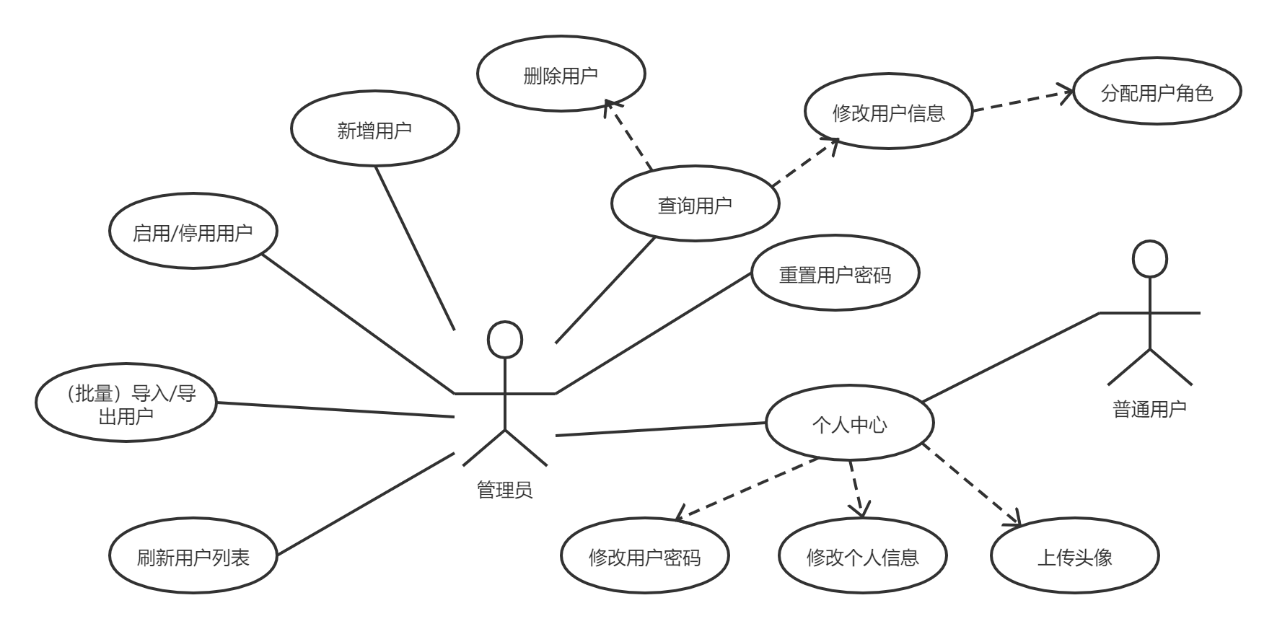
\includegraphics[width=0.85\textwidth]{figures/fig3-1.png}
  \caption{用户管理功能用例分析图}
  \label{fig3-1}
\end{figure}

\subsection{角色管理功能用例分析}
只有系统管理员能对系统角色进行管理。管理员可对系统所有角色进行如下操作：

1）对全部角色进行分页查询，也可根据需要通过角色名、角色状态、创建时间等进行条件查询；

2）新增系统角色，能够直接选择该角色可访问的功能菜单；

3）可修改查询出来的角色信息；

4）能够进行单一或批量角色删除；

5）能够停用或启用角色。

如图 \ref{fig3-2} 所示。

\begin{figure}[H]
  \centering
  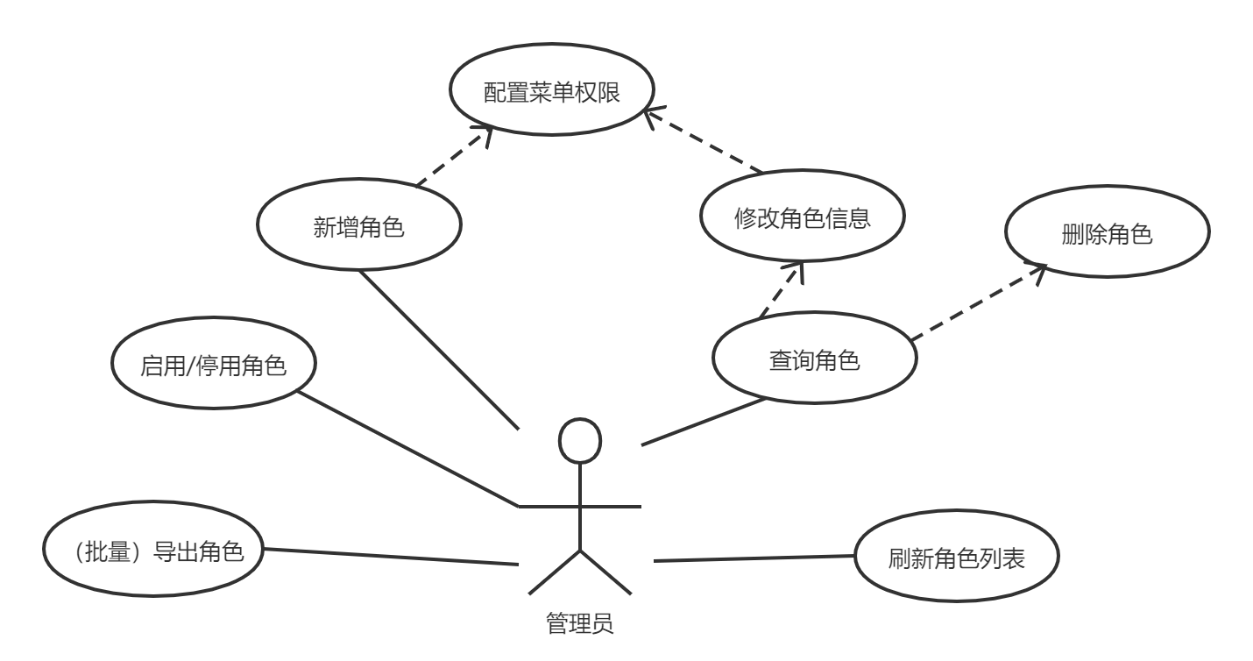
\includegraphics[width=0.85\textwidth]{figures/fig3-2.png}
  \caption{角色管理功能用例分析图}
  \label{fig3-2}
\end{figure}

\subsection{系统参数设置功能用例分析}
系统的参数设置功能能够动态地配置参数，在根据实际需求改变某些系统配置时不需要重新修改后台配置文件，也不需要重启后台服务。

该功能能够查看、新增、修改、删除系统配置参数。当修改参数后系统未做出相应改变，可点击清理缓存使参数生效。用户还可根据需要通过导出参数对系统参数进行保存。如图 \ref{fig3-3} 所示。

\begin{figure}[H]
  \centering
  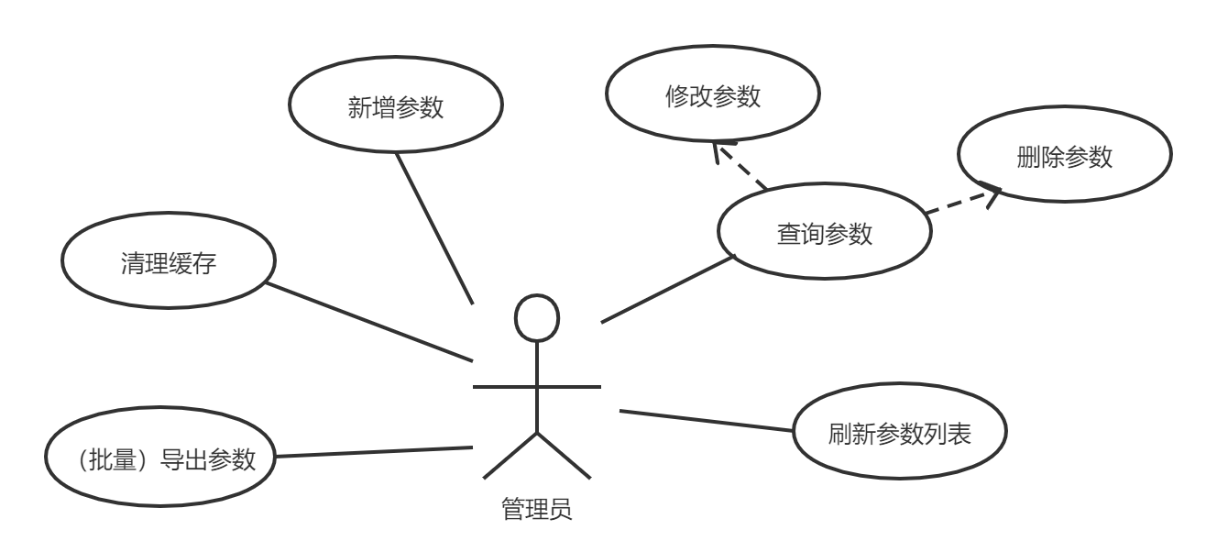
\includegraphics[width=0.85\textwidth]{figures/fig3-3.png}
  \caption{系统参数设置功能用例分析图}
  \label{fig3-3}
\end{figure}

\subsection{系统日志功能用例分析}
系统登录日志能够记录所有本系统使用者的登录信息。管理员或用户在登陆系统时会产生登录日志，管理员能够随时查看登录系统的用户。

登录日志中记录登录者的登录信息，管理员能够根据需求通过登录地址、用户名等条件对记录进行查询。在记录量过大时，用户能够导出登录记录，随后可删除部分或直接清空全部记录。如图 \ref{fig3-4} 所示。

\begin{figure}[H]
  \centering
  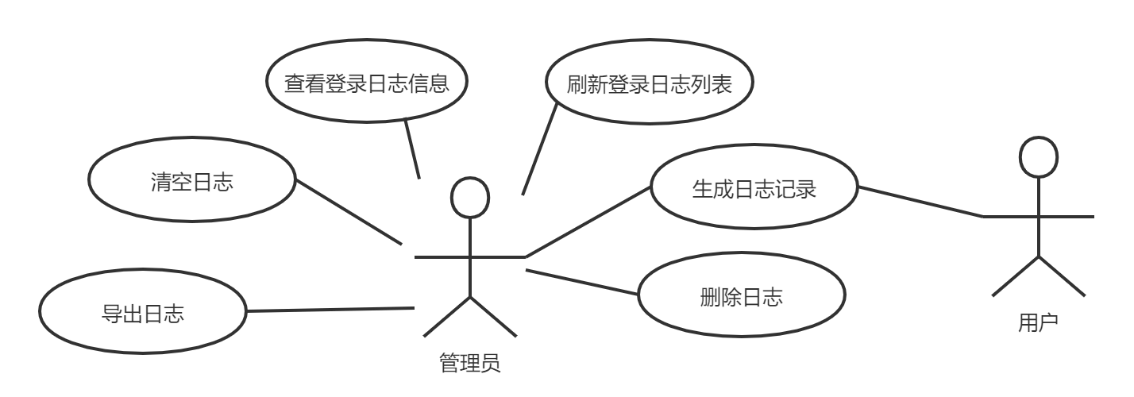
\includegraphics[width=0.85\textwidth]{figures/fig3-4.png}
  \caption{系统登录日志功能用例分析图}
  \label{fig3-4}
\end{figure}

系统操作日志记录登录者在登录系统后进行的所有操作。管理员或用户在登录系统后的所有操作都会产生记录，管理员可根据需要通过条件查询操作记录。

管理员能够根据需要导出操作日志，删除部分或直接清空全部记录，也可以点击刷新按钮刷新操作日志数据，还能够查看每一个操作详情，在系统出现 bug 时便于对系统进行维护。

当系统遭遇攻击时，管理员能够通过登录日志和操作日志快速锁定攻击 IP 并找出攻击者的目的。如图 \ref{fig3-5} 所示。

\begin{figure}[H]
  \centering
  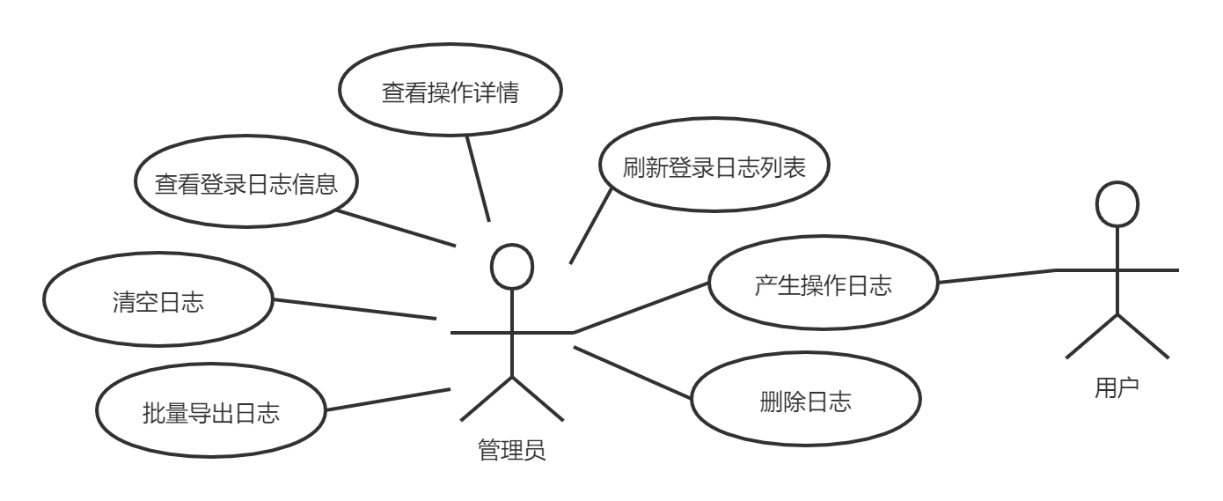
\includegraphics[width=0.85\textwidth]{figures/fig3-5.png}
  \caption{系统操作日志功能用例分析图}
  \label{fig3-5}
\end{figure}

\subsection{上传下载功能用例分析}
用户和管理员可通过上传功能上传自己的头像等，通过下载功能可下载已导出的数据文件和生成的代码文件。如图 \ref{fig3-6} 所示。

\begin{figure}[H]
  \centering
  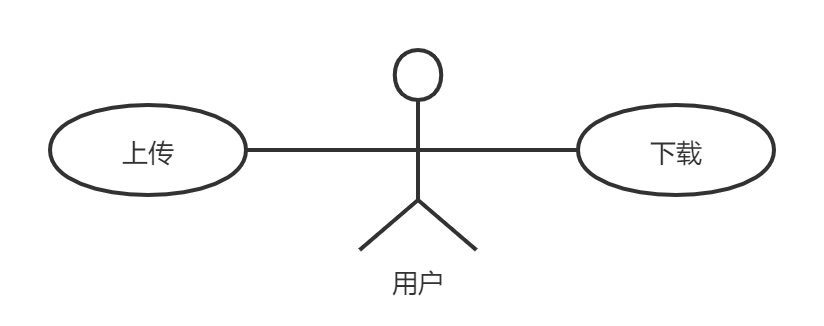
\includegraphics[width=0.6\textwidth]{figures/fig3-6.png}
  \caption{上传下载功能用例分析图}
  \label{fig3-6}
\end{figure}

\subsection{创建数据表功能用例分析}
用户在创建数据表时需要先添加数据表字段，然后完善字段信息，能够选择该字段是否为主键、是否必填等。在完成数据表编辑后，用户可通过提交数据表信息将数据表加入数据库并生成 SQL 脚本。如图 \ref{fig3-7} 所示。

\begin{figure}[H]
  \centering
  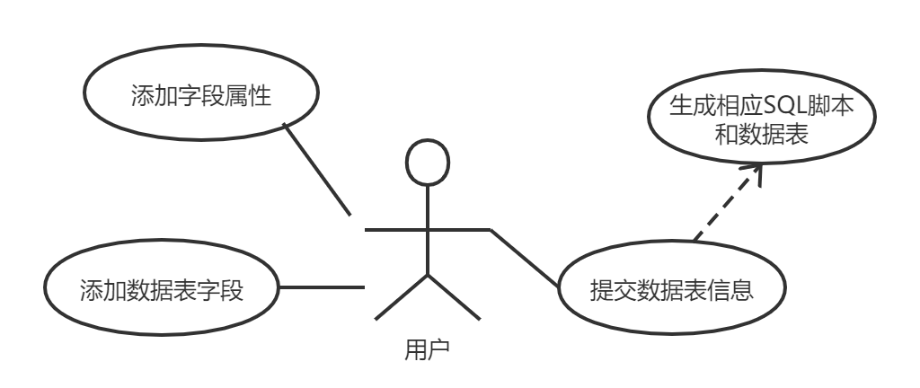
\includegraphics[width=0.75\textwidth]{figures/fig3-7.png}
  \caption{创建数据表功能用例分析}
  \label{fig3-7}
\end{figure}

\subsection{编辑生成配置功能用例分析}
在用户创建数据表后，通过导入数据表就可对改表生成代码进行个人配置。在基本信息中，用户能够对生成的 Java 代码实体类名称、表名和作者名进行编辑。在字段信息页内，用户可以编辑该数据表字段对应的 Java 字段名、Java 字段属性等，然后选择该字段可进行的操作（查询、新增、修改、列表展示）；在查询操作中用户可选择精确查询、模糊查询、范围查询等；对于操作页面表单，可选择字段是否必填、该字段在页面内的表现形式（输入框、下拉框、日期选择器等），对于状态码类型的字段还能够选择相应的数据字典对字段进行解释。

在生成信息内，用户可以选择模板的类型、生成文件的路径及模块名等文件属性。如图 \ref{fig3-8} 所示。

\begin{figure}[H]
  \centering
  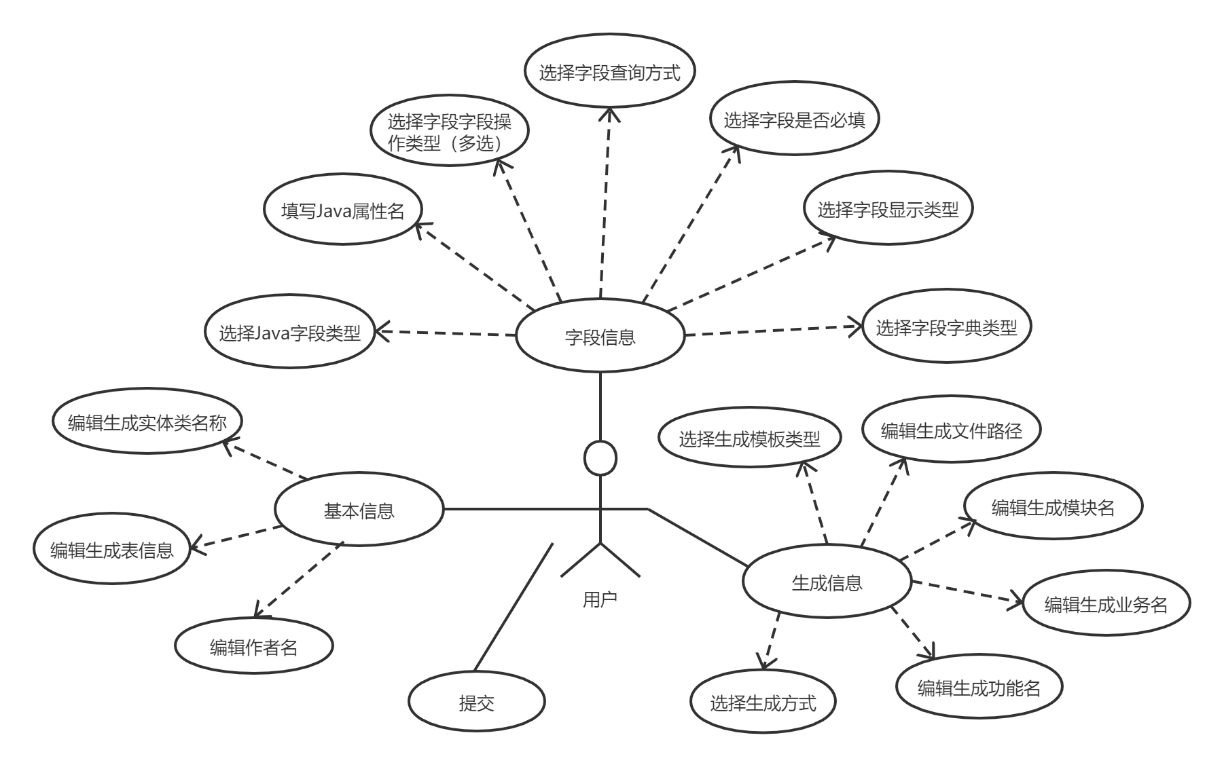
\includegraphics[width=0.85\textwidth]{figures/fig3-8.png}
  \caption{编辑生成配置功能用例分析图}
  \label{fig3-8}
\end{figure}

\subsection{代码预览功能用例分析}
在导入创建的数据表后，用户可在相应列表项后的操作中点击预览，系统通过弹窗展示生成的代码。

展示的代码包括 Java 文件、MyBatis 文件、SQL 脚本文件、前端页面文（.vue）和脚本文件（.js），其中 Java 文件包含从实体类到接口共五个文件。

生成的代码遵循统一的编码规范，并且结构符合 MVC 三层结构；在编辑生成配置后能够实时更新预览的代码。如图 \ref{fig3-9} 所示。

\begin{figure}[H]
  \centering
  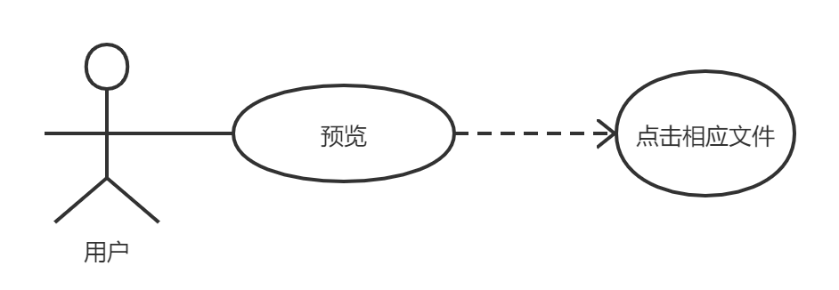
\includegraphics[width=0.7\textwidth]{figures/fig3-9.png}
  \caption{代码预览功能用例分析图}
  \label{fig3-9}
\end{figure}

\subsection{数据同步功能用例分析}
用户在修改已导入的数据表后，可通过点击同步数据按钮完成对系统数据表的更新。在更新完成后，系统会重新查询数据表信息并完成生成代码配置的更新。如图 \ref{fig3-10} 所示。

\begin{figure}[H]
  \centering
  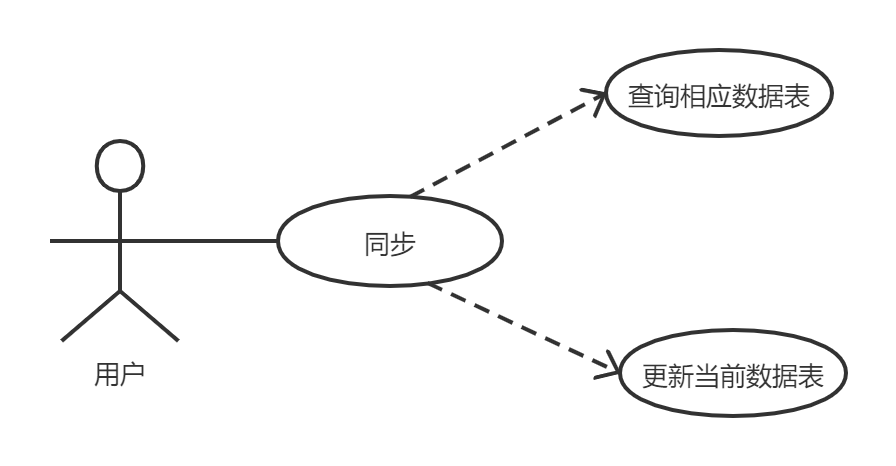
\includegraphics[width=0.7\textwidth]{figures/fig3-10.png}
  \caption{数据同步功能用例分析图}
  \label{fig3-10}
\end{figure}

\subsection{代码生成功能用例分析}
在用户完成配置等工作后，点击生成代码按钮，系统会根据用户的配置动态地组成相应文件，然后生成配置的文件路径并将文件存入，在生成路径的根目录下打包。随后用户便通过浏览器发出请求进行下载。如图 \ref{fig3-11} 所示。

\begin{figure}[H]
  \centering
  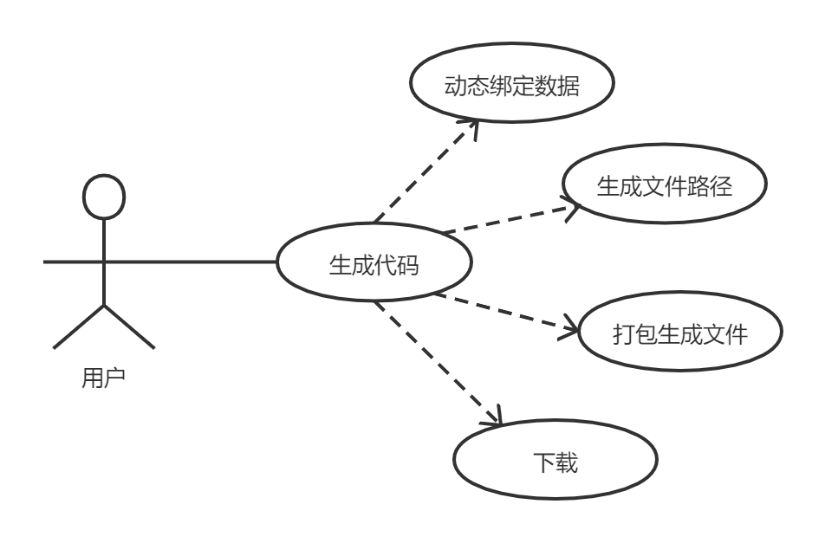
\includegraphics[width=0.7\textwidth]{figures/fig3-11.png}
  \caption{代码生成功能用例分析图}
  \label{fig3-11}
\end{figure}

\subsection{组件拖拽功能用例分析}
用户可根据此功能实现对页面的个性化构建。系统会列出构成页面的组件（布局容器、文本框、日期选择器、上传等），用户通过鼠标左键单击组件，该组件会自动放入页面布局框；用户也可以通过按住鼠标左键将组件拖入页面布局框内。如图 \ref{fig3-12} 所示。

\begin{figure}[H]
  \centering
  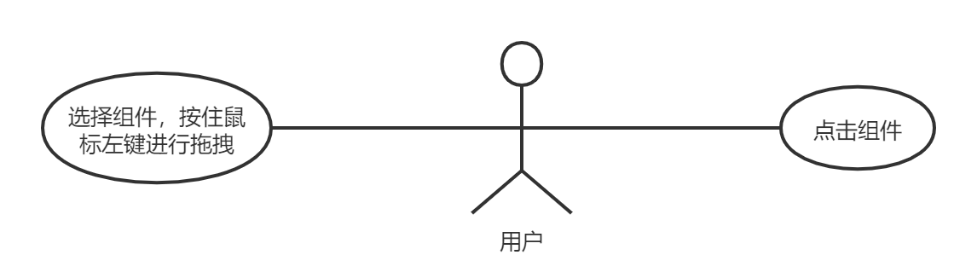
\includegraphics[width=0.75\textwidth]{figures/fig3-12.png}
  \caption{组件拖拽功能用例分析图}
  \label{fig3-12}
\end{figure}

\subsection{组件属性编辑功能用例分析}
用户在完成页面组件选择后，可通过右侧组件属性栏对组件的属性进行编辑。用户使用鼠标左键单击已选择的组件，右侧会展示该组件拥有的属性（组件类型、字段名、标题、占位提示、栅格大小、默认值、前后图表、字数限制、能否清空、是否只读、是否禁用、是否必填及正则验证等）。

用户根据实际需求可通过编辑这些属性完成对组件细节上的调整。对已选择的单个组件可通过组件边框上的按钮进行复制或者删除。如图 \ref{fig3-13} 所示。

\begin{figure}[H]
  \centering
  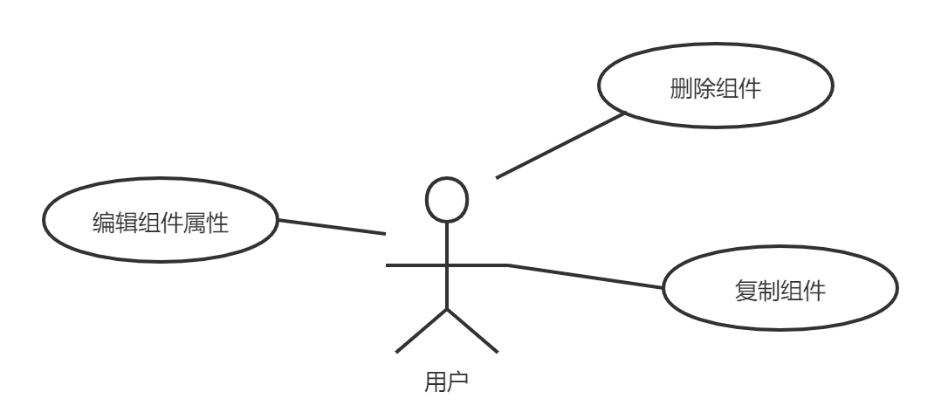
\includegraphics[width=0.75\textwidth]{figures/fig3-13.png}
  \caption{组件属性编辑功能用例分析图}
  \label{fig3-13}
\end{figure}

\subsection{页面属性编辑功能用例分析}
用户通过此功能可对构建的页面的整体属性进行编辑。主要分为展示页和表单页：展示页中包含页面名称、页面尺寸、对齐方式、栅格间距等属性；表单页则包含表单名、表单模型、校验模型、表单尺寸、标签对齐方式及标签宽度、栅格间隔、是否禁用表单等属性。

从页面构建开始到页面完成之后，用户随时可导出页面文件（.vue）、复制代码或清空页面元素。在导出代码时可选择导出为页面或弹窗。如图 \ref{fig3-14} 所示。

\begin{figure}[H]
  \centering
  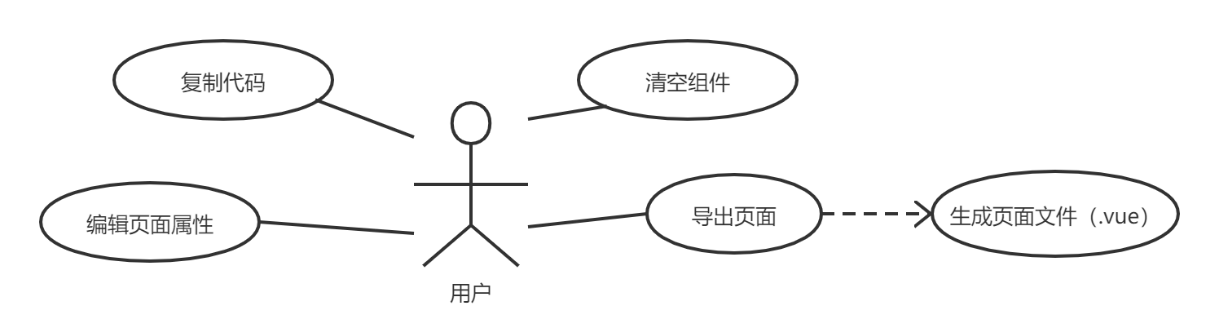
\includegraphics[width=0.85\textwidth]{figures/fig3-14.png}
  \caption{页面属性编辑功能用例分析图}
  \label{fig3-14}
\end{figure}

\subsection{在线预览功能用例分析}
从页面构建开始到页面完成之后，用户可随时通过此功能对当前页面进行在线编译。系统可直接展示编译后的页面，用户则可直接对此页面进行操作、调试等，或直接对编译页面的代码进行修改。如图 \ref{fig3-15} 所示。

\begin{figure}[H]
  \centering
  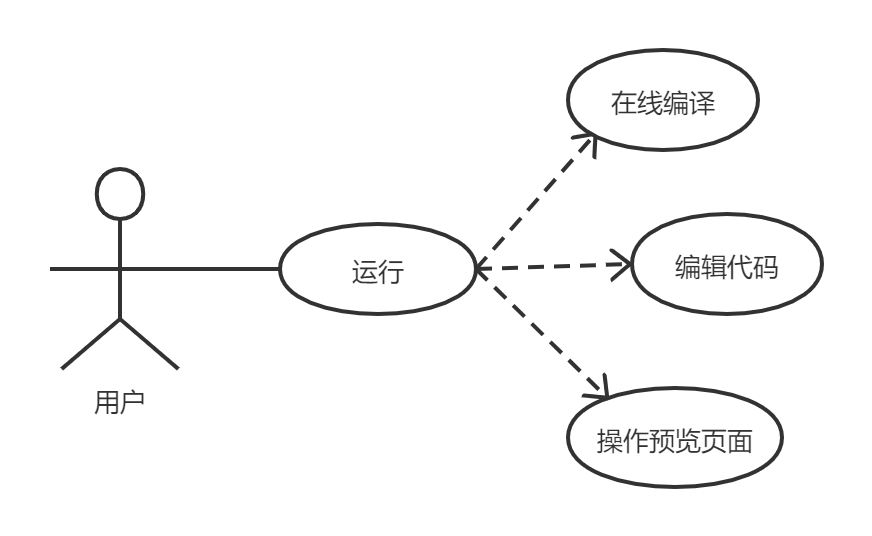
\includegraphics[width=0.7\textwidth]{figures/fig3-15.png}
  \caption{在线预览功能用例分析图}
  \label{fig3-15}
\end{figure}

\subsection{界面模板功能用例分析}
此功能主要展示已完成构建的页面。用户可通过点击界面模板对页面进行查看，并可通过点击下载按钮直接下载该模板。

用户也可将自己构建的页面进行分享，系统将自动将其页面添加至界面模板功能中，其他用户可通过界面模板功能进行查看。如图 \ref{fig3-16} 所示。

\begin{figure}[H]
  \centering
  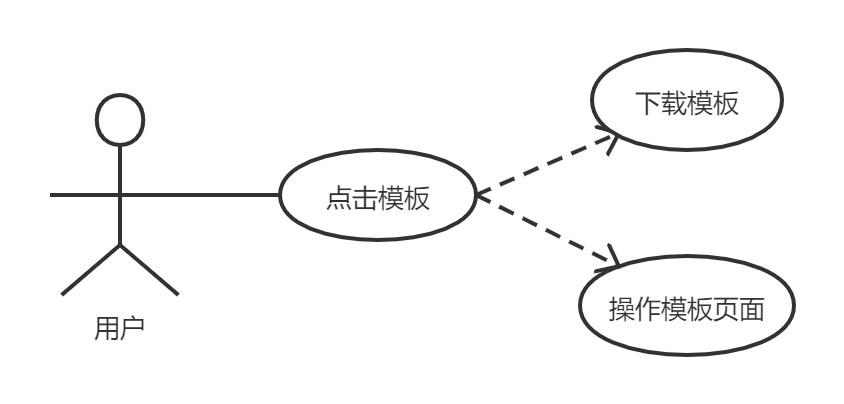
\includegraphics[width=0.7\textwidth]{figures/fig3-16.png}
  \caption{界面模板功能用例分析图}
  \label{fig3-16}
\end{figure}

\chapter{系统设计}

\section{系统整体架构}
基于 SpringCloud 的企业系统自动生成平台（以下简称“平台”）整体上采用了微服务架构设计。后台则采用多模块结构进行项目结构划分，将每一个服务作为一个模块进行构建，每一个服务内部采用 SpringBoot 架构进行具体实现。

在启动系统后，系统访问 Nacos 完成服务的注册、监控、跟踪，随后获取 Nacos 中的服务配置完成项目启动及初始化。

用户在登陆平台时请求将先通过认证中心，通过认证后访问系统服务进行登录验证。通过 API Gateway 网关对所有 HTTP 请求进行处理调度，根据服务配置将请求发往相应服务后台接口，经过微服务架构中的 Module 层的逻辑处理后完成对数据库的操作，然后返回结果到前端页面中。如图 \ref{fig4-1} 所示。

\begin{figure}[H]
  \centering
  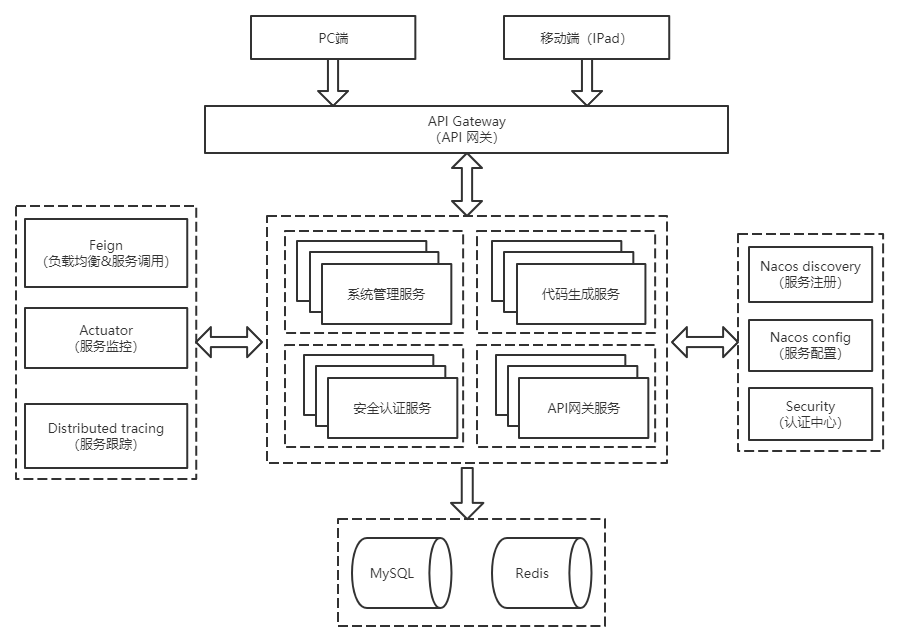
\includegraphics[width=0.85\textwidth]{figures/fig4-1.png}
  \caption{系统架构图}
  \label{fig4-1}
\end{figure}

\section{系统功能划分}
根据平台需求进行分析，在此基础上实现对平台功能的设计。本课题将平台主要划分为系统管理模块、代码生成模块、页面构建模块以及界面模板模块。

系统管理模块主要负责针对系统用户和角色的配置管理以及系统参数和登录、操作日志的查看。

代码生成模块负责从创建数据表、配置生成属性到代码生成的全部操作，其中包含上传下载功能、创建数据表功能、编辑生成配置功能、代码预览功能、数据同步功能、代码生成功能。该模块是平台的核心模块。

页面构建模块主要包括用户通过拖拽组件功能，编辑组件和页面属性功能实现个性化页面构建，并可通过在线编译功能进行预览。

界面模板模块负责平台中已经构建完成的模板界面的管理，用户在完成页面后也可选择将自己的页面共享，添加到界面模板中。如图 \ref{fig4-2} 所示。

\begin{figure}[H]
  \centering
  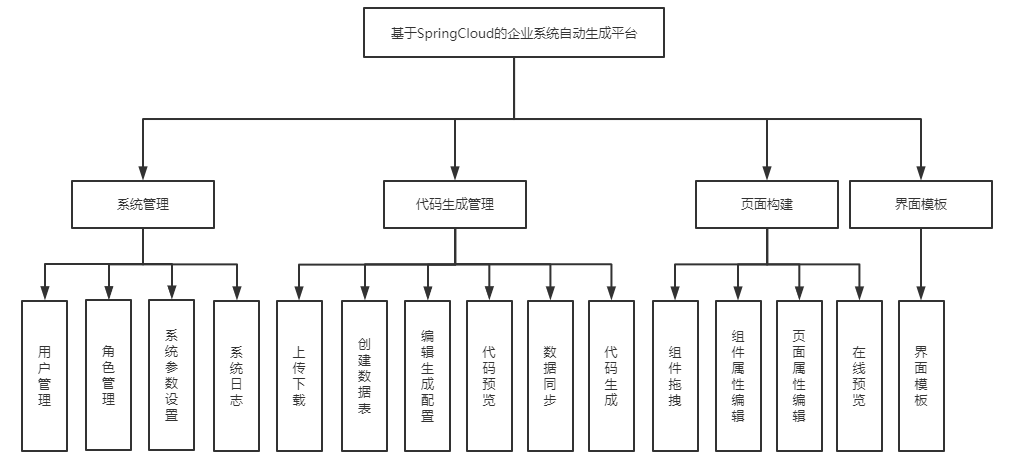
\includegraphics[width=0.9\textwidth]{figures/fig4-2.png}
  \caption{系统功能图}
  \label{fig4-2}
\end{figure}

\section{功能详细设计}

\subsection{用户管理功能}
管理员在进入用户管理页后，系统会自动调用 SysUserController 中的查询接口，查询系统用户数据。

在管理员点击新增按钮将数据插入到后端时，会在 SysUserService 中判断新增用户信息中与数据库中是否存在重复数据。如果重复则在前端页面进行提示，否则调用插入方法完成插入数据操作并返回成功结果；在插入成功后根据插入的数据将用户数据和其对应的角色进行关联，成功后返回结果到前端页面。

在修改用户信息时，同样会在 SysUserService 中进行验重，如果涉及修改用户角色变化则调用修改用户角色关联表方法对用户的角色进行修改。

删除用户直接进行物理删除，并根据该用户 id 对该用户和角色的关联数据进行同步删除。如图 \ref{fig4-3} 所示。

\begin{figure}[H]
  \centering
  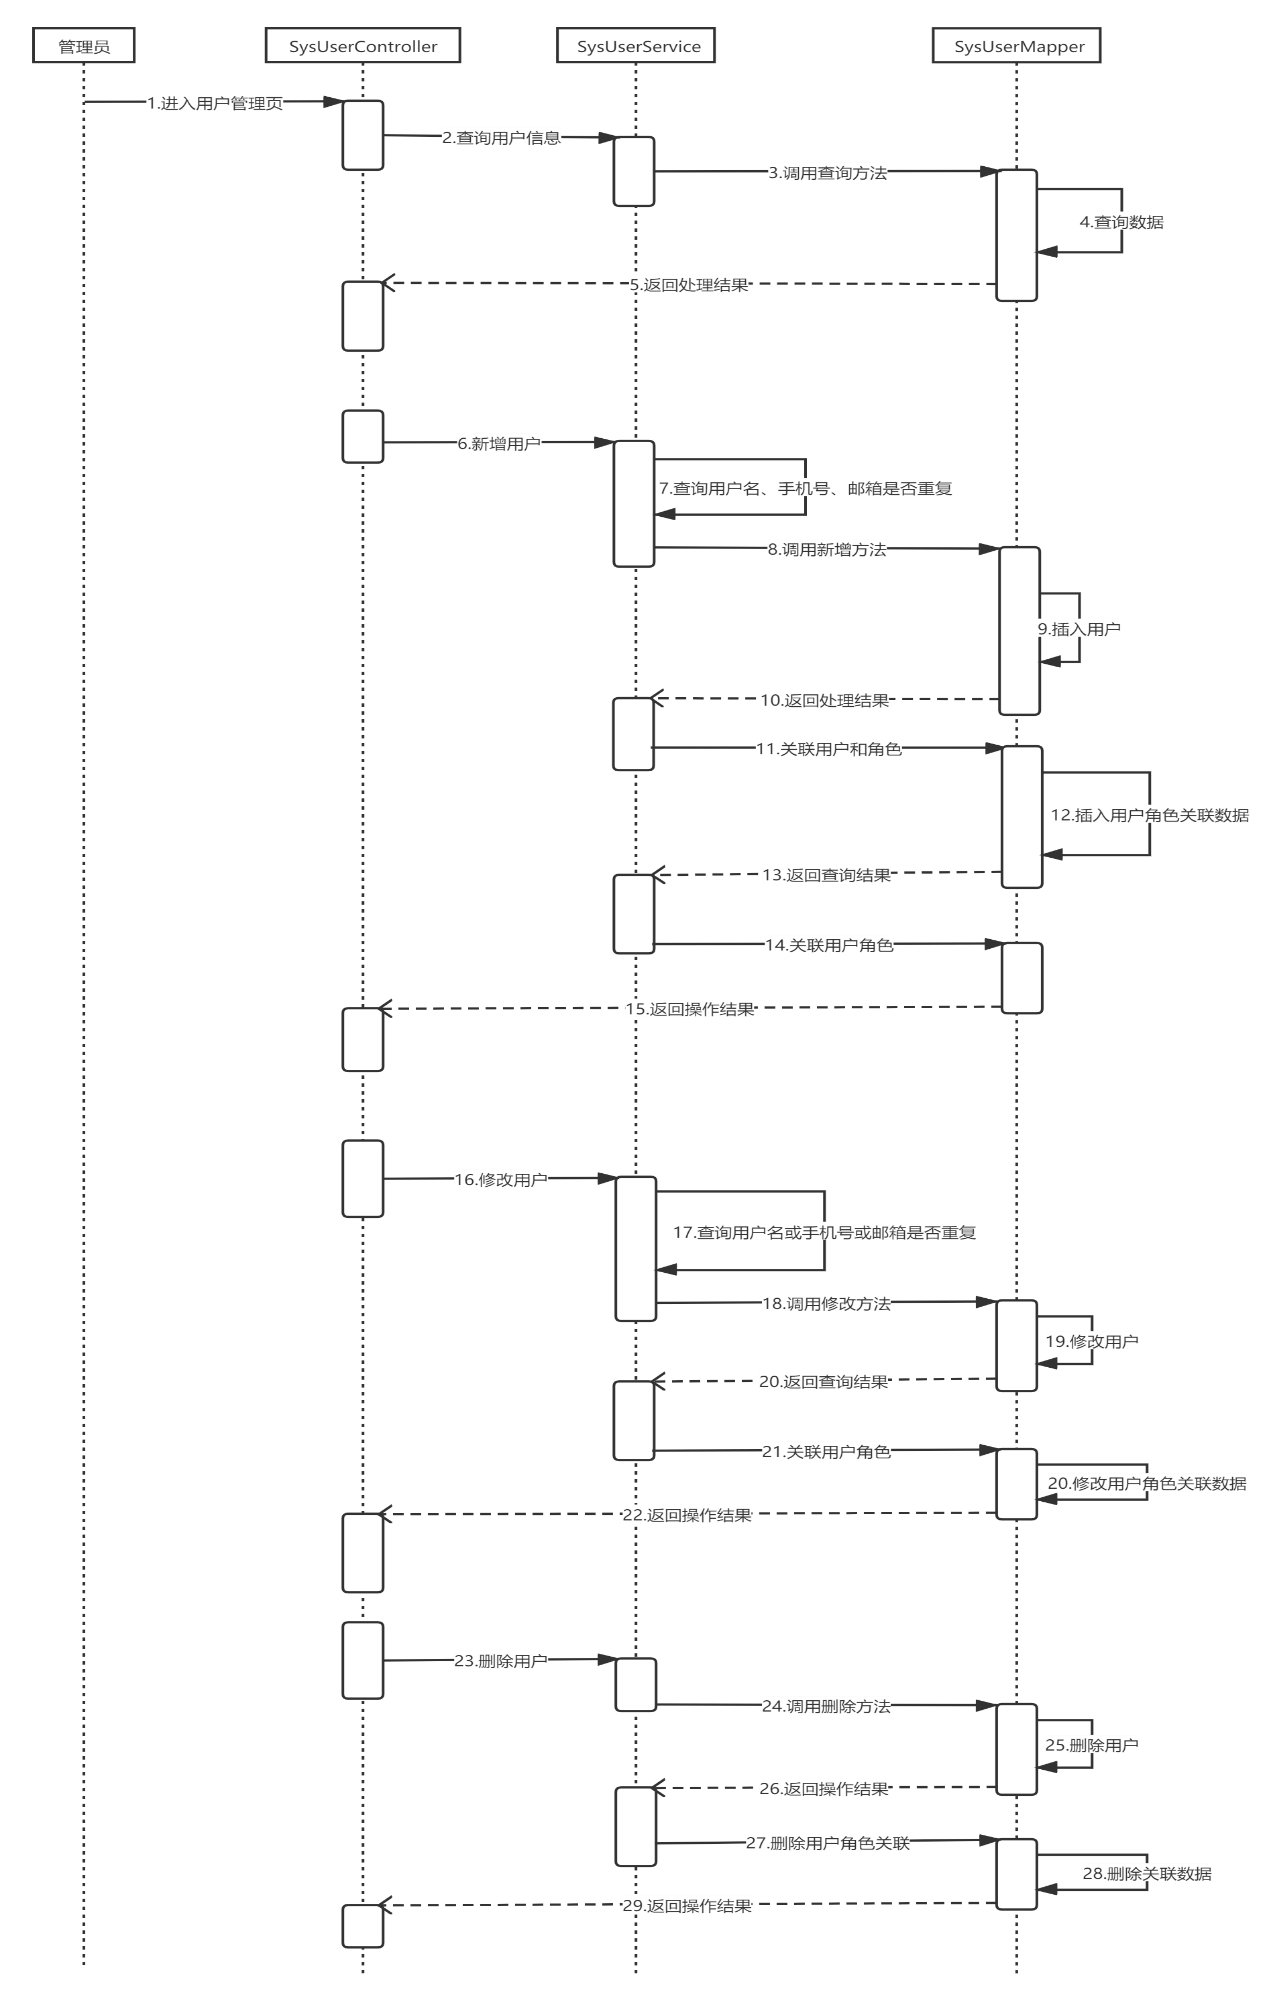
\includegraphics[height=0.82\textheight]{figures/fig4-3.png}
  \caption{用户管理功能时序图}
  \label{fig4-3}
\end{figure}

\subsection{角色管理功能}
管理员在进入角色管理页后，系统会自动调用 SysRoleController 中的查询接口，查询系统角色数据。

在管理员点击新增按钮将数据传到后端时，会在 SysRoleService 中判断新增角色信息中与数据库中是否存在重复数据。如果重复则在前端页面进行提示，否则调用插入方法完成插入数据操作并返回成功结果；在插入成功后根据插入的数据判断将角色数据和其对应的菜单数据进行关联，成功后返回结果到前端页面。

在修改角色信息时，同样会在 SysRoleService 中进行验重，如果涉及修改角色菜单权限的变化，则调用修改角色菜单关联表方法对角色的菜单权限进行修改。

删除角色直接进行物理删除，并根据该角色 id 对该角色和菜单的关联数据进行同步删除。如图 \ref{fig4-4} 所示。

\begin{figure}[H]
  \centering
  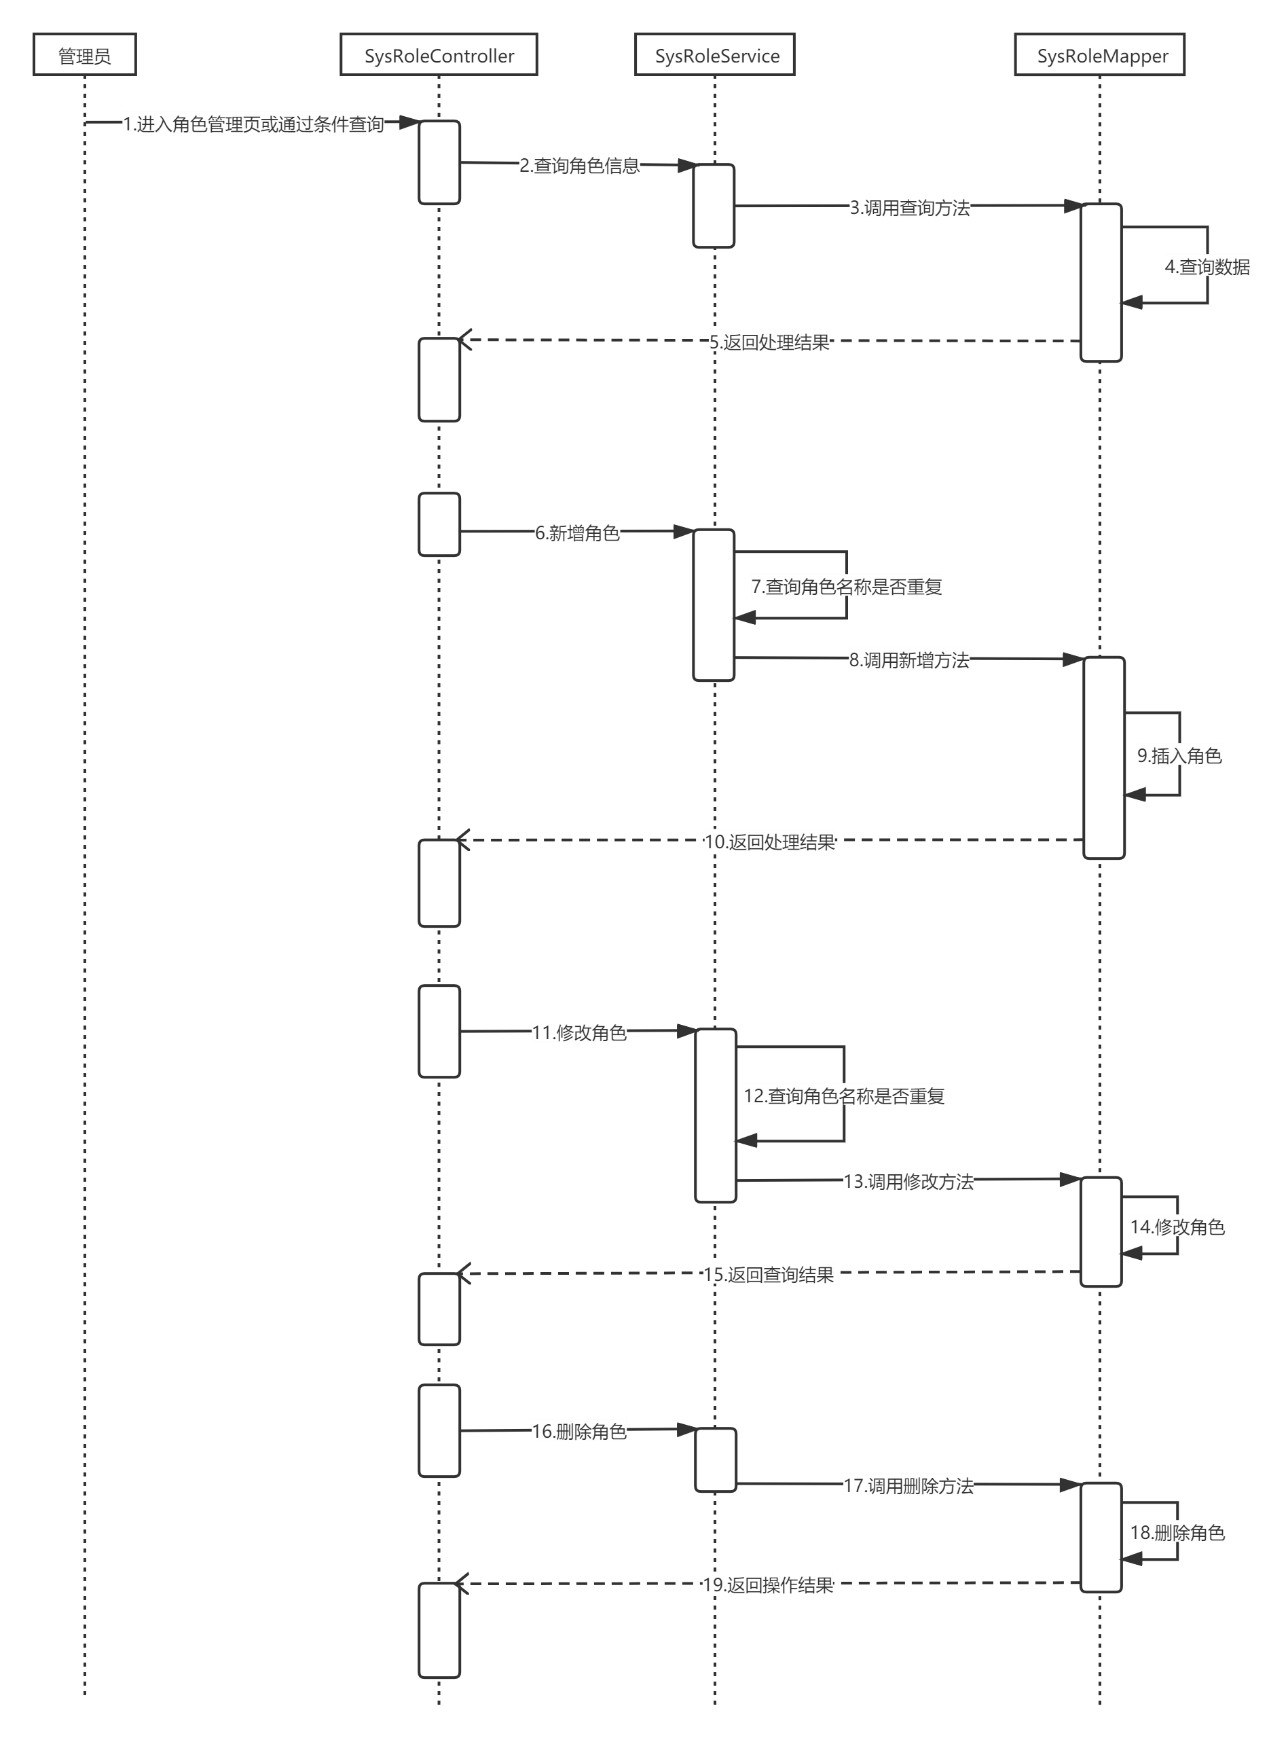
\includegraphics[height=0.82\textheight]{figures/fig4-4.png}
  \caption{角色管理功能时序图}
  \label{fig4-4}
\end{figure}

\subsection{系统参数设置功能}
管理员进入系统参数设置页面时，系统调用 SysConfigController 中的查询接口，将所有已配置的系统参数通过列表展示出来。管理员也可以通过选择条件对参数数据进行查询。

管理员新增系统参数时会在 SysConfigService 层中调用 SQL 插入方法将新增配置插入数据库。

修改或删除时则是根据修改数据的主键 id 找到相应的数据并进行修改或删除。如图 \ref{fig4-5} 所示。

\begin{figure}[H]
  \centering
  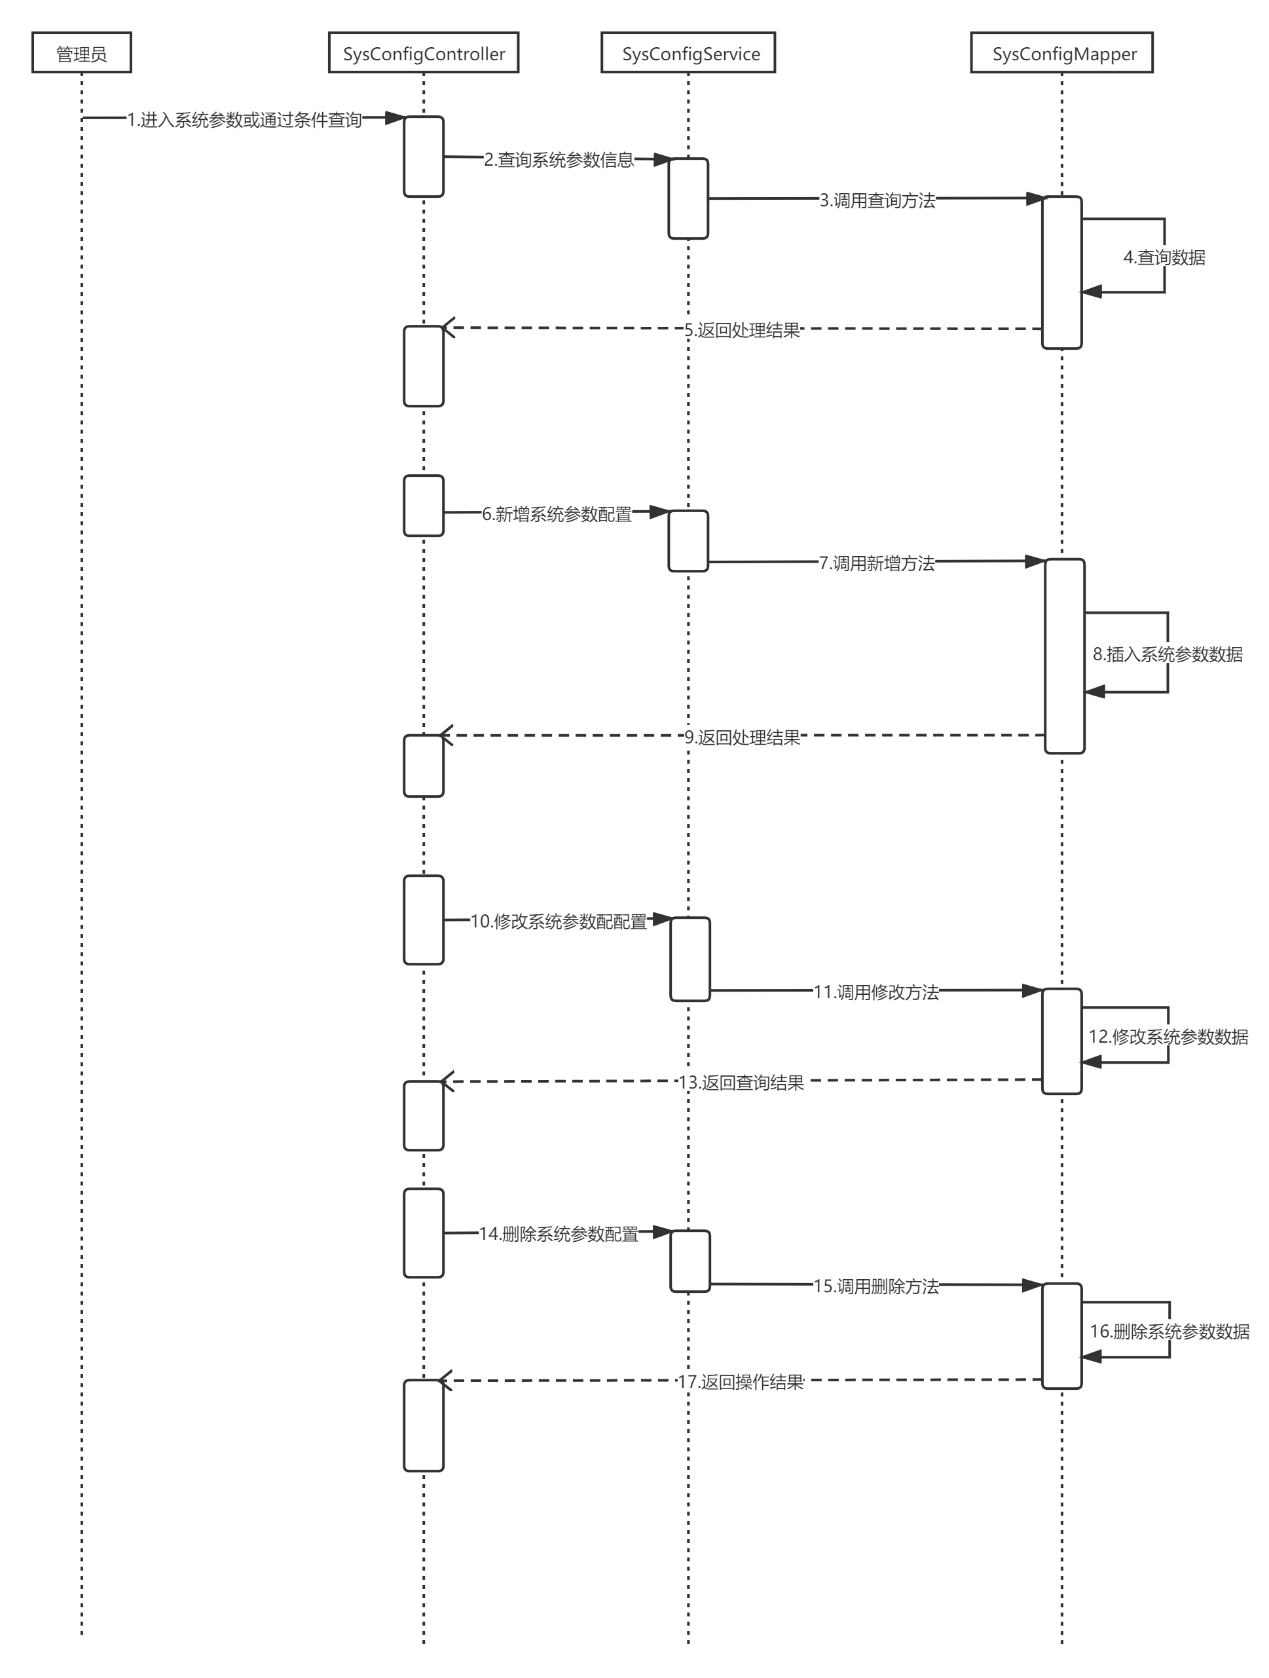
\includegraphics[height=0.82\textheight]{figures/fig4-5.png}
  \caption{系统参数配置功能时序图}
  \label{fig4-5}
\end{figure}

\subsection{系统日志功能}
在管理员进入系统日志界面后可选择查看登录日志或操作日志。

点击查看登录日志后，系统根据参数查询用户登录系统的登录日志数据。当用户或管理员每次进行登录操作后，都会调用 SysLogController 中的新增日志方法。在 SysLogService 层中，后端会先获取登陆者的信息，保存后则调用日志插入方法，将登录信息存入数据表中。

用户或管理员在对系统进行操作后会调用插入操作日志接口，获取登录人的信息，并在存入对象后调用插入操作日志方法，将操作者的信息和操作的方法等存入数据表中。

在查询出日志列表后，用户可通过勾选数据前方的复选框对数据进行删除。系统将选中数据的 id 存入数组并传回后端，后端根据调用接口对数据进行批量删除操作。

当数据量过大时，用户可通过导出功能将日志数据导出为 Excel，然后点击清空按钮可一次清空全部日志数据。如图 \ref{fig4-6} 所示。

\begin{figure}[H]
  \centering
  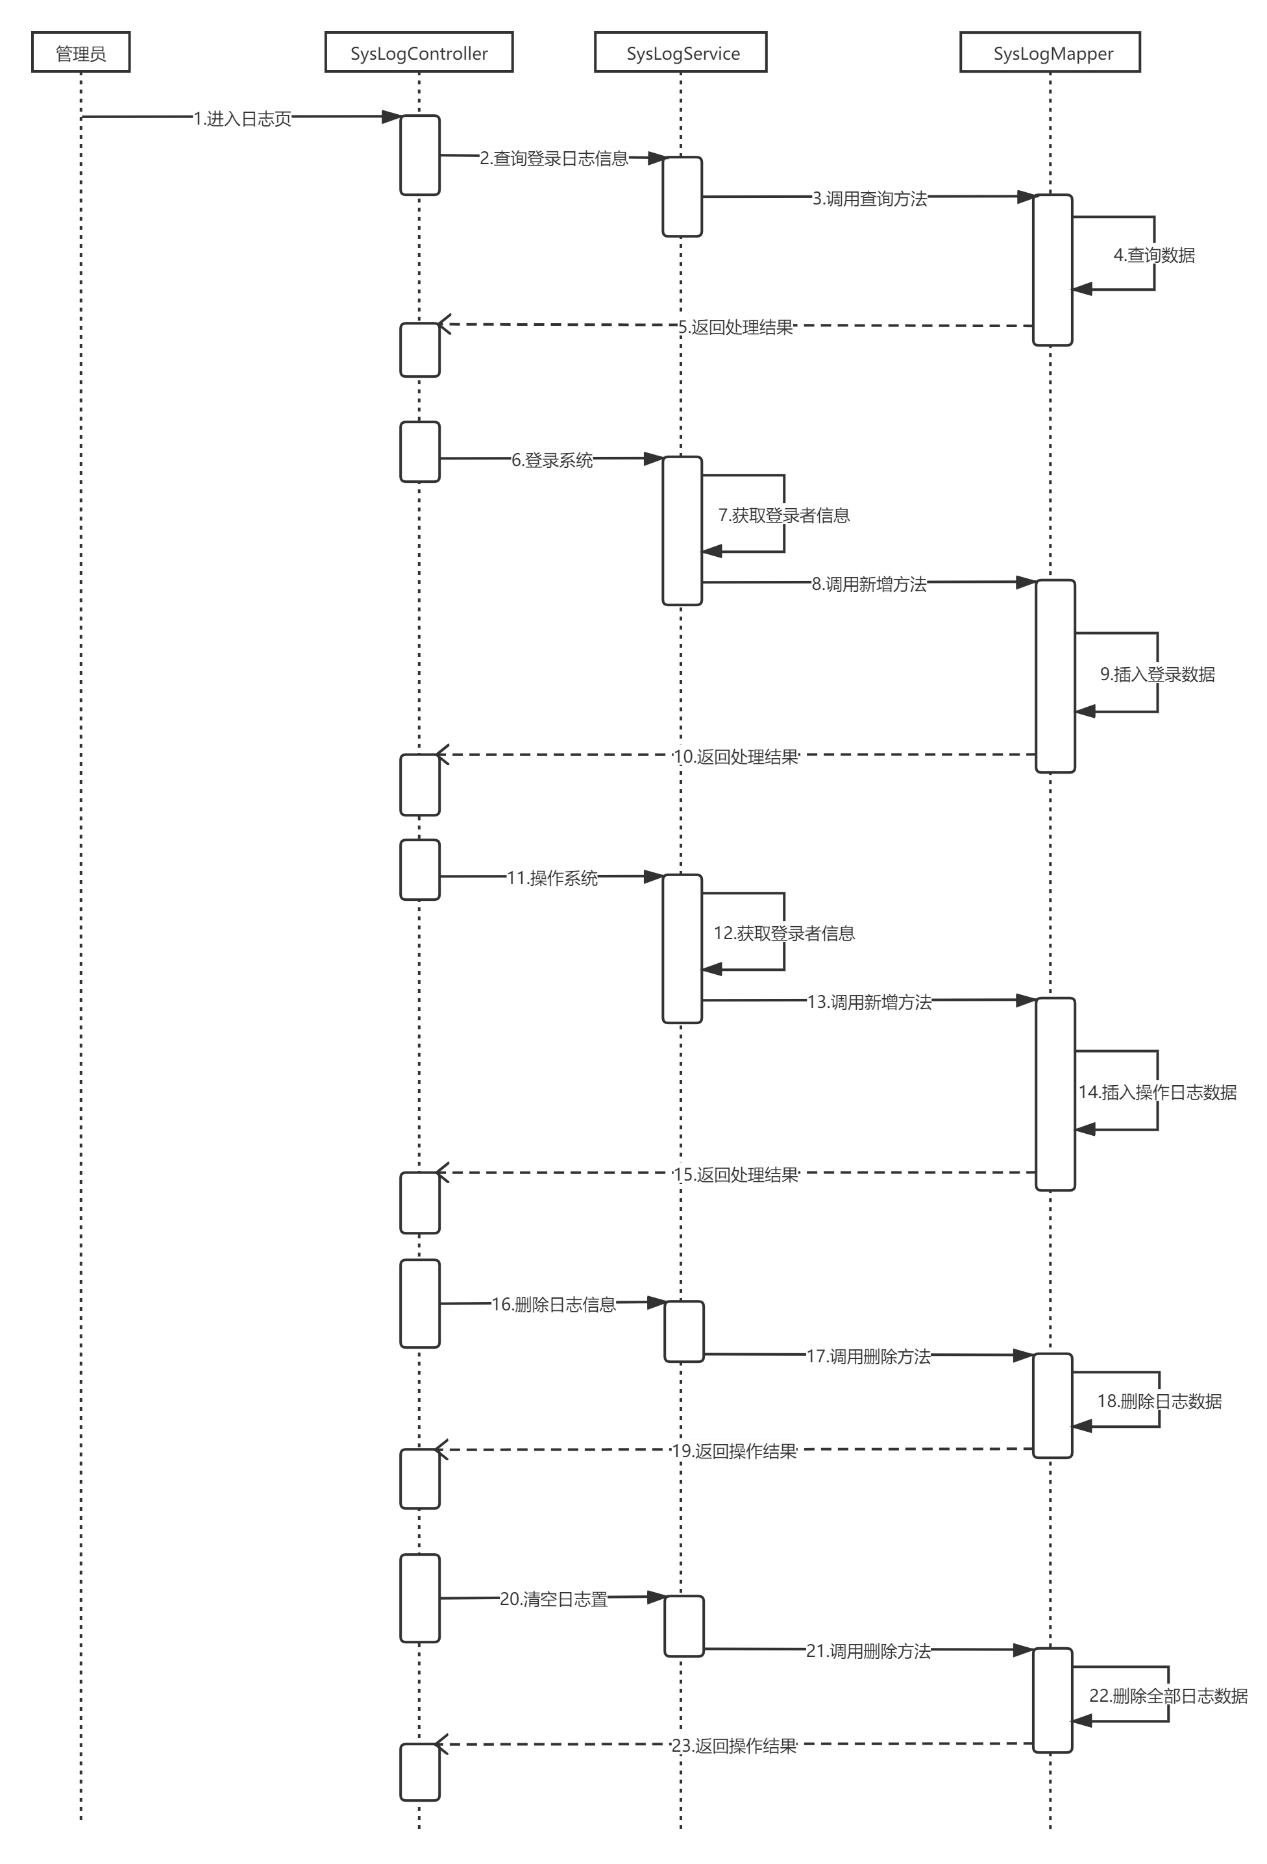
\includegraphics[height=0.82\textheight]{figures/fig4-6.png}
  \caption{系统日志功能时序图}
  \label{fig4-6}
\end{figure}

\subsection{上传下载功能}
在执行上传头像等操作时均会调用 CommonController 中的上传接口处理文件。

上传时调用 FileUploadUtils（文件上传工具类）中的上传方法，后端对文件名进行 UUID 编码后结合当天日期生成文件路径。然后，系统会将文件上传至服务器，成功后将新文件名和文件路径返回前端页面。

用户在生成代码、导出页面文件、下载页面模板时调用查询文件接口，将查询出的文件路径和文件名等信息返回页面中，用户点击文件链接即可发起浏览器下载请求实现下载。如图 \ref{fig4-7} 所示。

\begin{figure}[H]
  \centering
  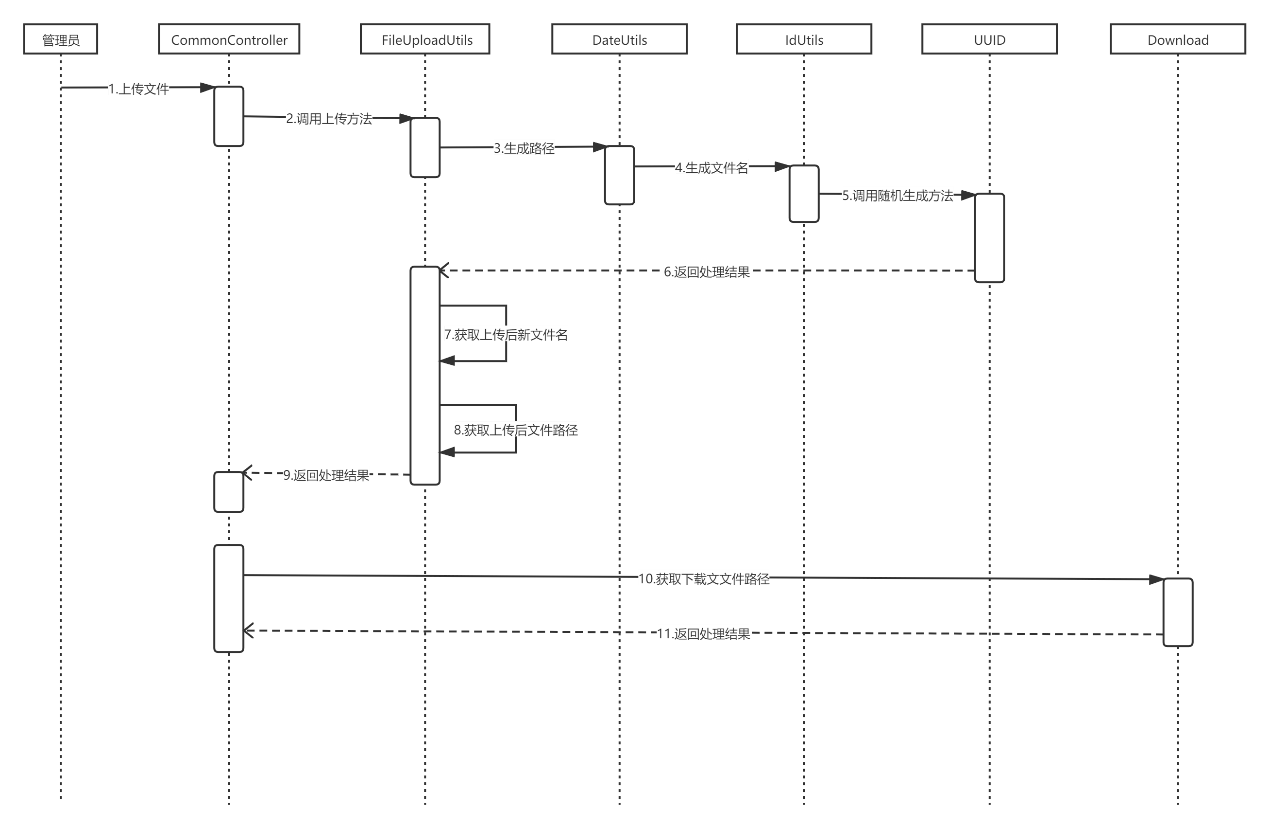
\includegraphics[width=0.75\textwidth]{figures/fig4-7.png}
  \caption{上传下载功能时序图}
  \label{fig4-7}
\end{figure}

\subsection{创建数据表功能}
用户想要生成代码需要先创建相应的数据表。在页面中编辑完那些生成数据表的信息后，用户将调用后台 DataTableController 中的接口进行提交。后端将数据表信息动态存入创建数据表语句后调用创建方法，创建成功后将创建表的信息和用户 id 插入新增数据表记录表中。

对已创建数据表进行修改时可根据传回数据动态拼接修改表结构语句，修改成功后返回成功结果。

在删除数据表时，调用 DataTableController 中的删除接口，将数据表名作为参数调用删除表方法，完成后删除所创建的数据表记录表中对应的数据。如图 \ref{fig4-8} 所示。

\begin{figure}[H]
  \centering
  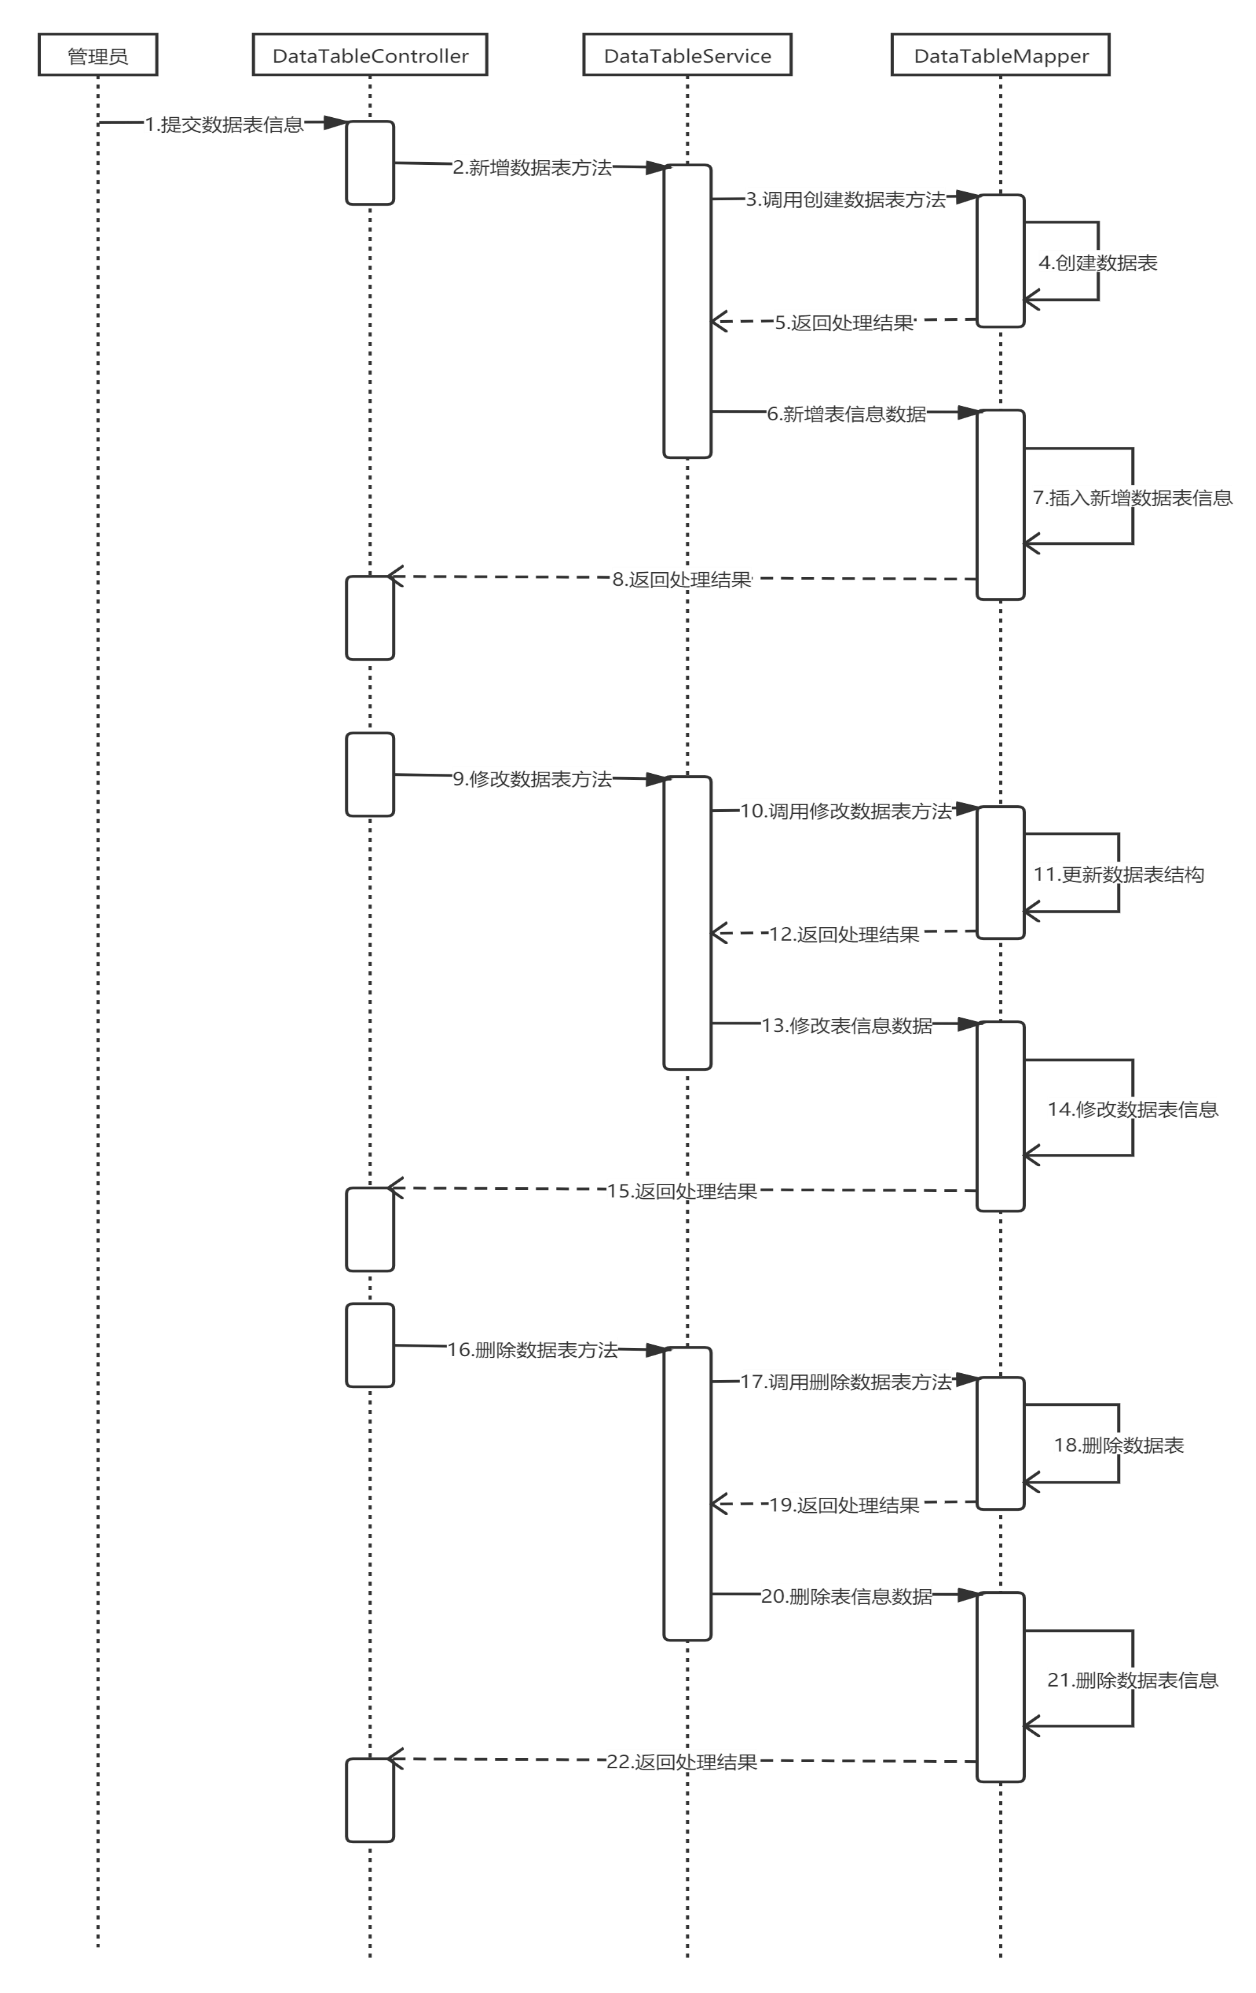
\includegraphics[height=0.82\textheight]{figures/fig4-8.png}
  \caption{创建数据表功能时序图}
  \label{fig4-8}
\end{figure}

\subsection{编辑生成配置功能}
用户导入要生成的数据表信息后，可对其生成的代码进行配置（生成路径、生成方式、字段属性等），完成配置后点击保存则调用后端 GenController 中的修改接口。该函数在 GenService 层中对生成信息进行验证（格式、非空等），验证通过后调用修改方法修改代码，生成业务表中的相应数据，成功后调用业务字段修改方法对代码生成字段表数据进行修改。如图 \ref{fig4-9} 所示。

\begin{figure}[H]
  \centering
  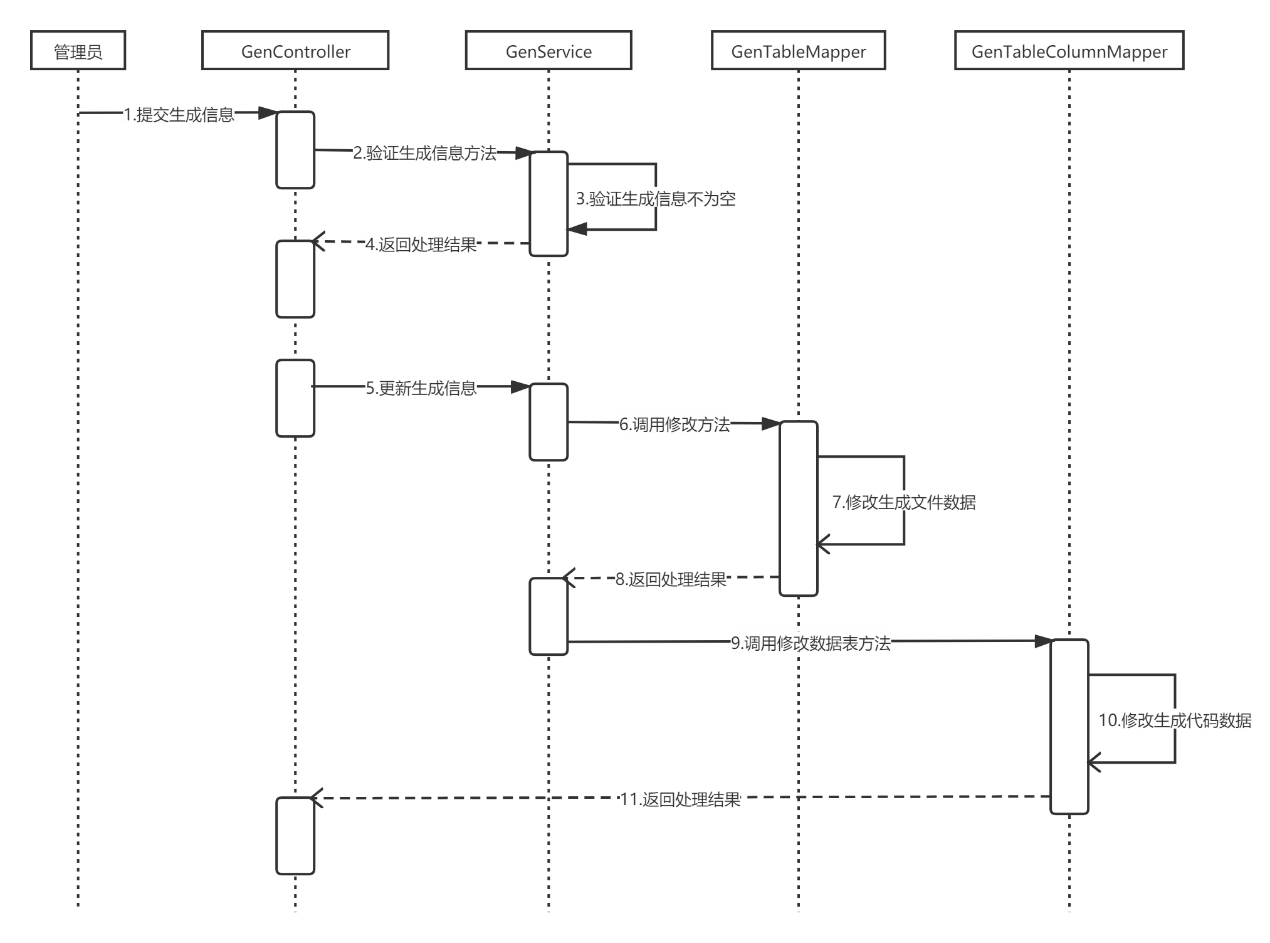
\includegraphics[width=0.8\textwidth]{figures/fig4-9.png}
  \caption{编辑生成配置功能时序图}
  \label{fig4-9}
\end{figure}

\subsection{代码预览功能}
用户点击预览代码就可以通过弹窗查看当前配置下生成的代码。点击预览后将访问 GenController 中的预览接口，然后以 id 为参数查询代码配置数据，将返回结果通过中间变量保存。

初始化 vm 模板方法，通过 VelocityInitializer 类中的加载方法加载 vm 文件，然后通过 VelocityUtils 工具类中的设置变量方法将保存的配置数据添加到 vm 模板相应位置，最后将设置完成的模板返回页面。如图 \ref{fig4-10} 所示。

\begin{figure}[H]
  \centering
  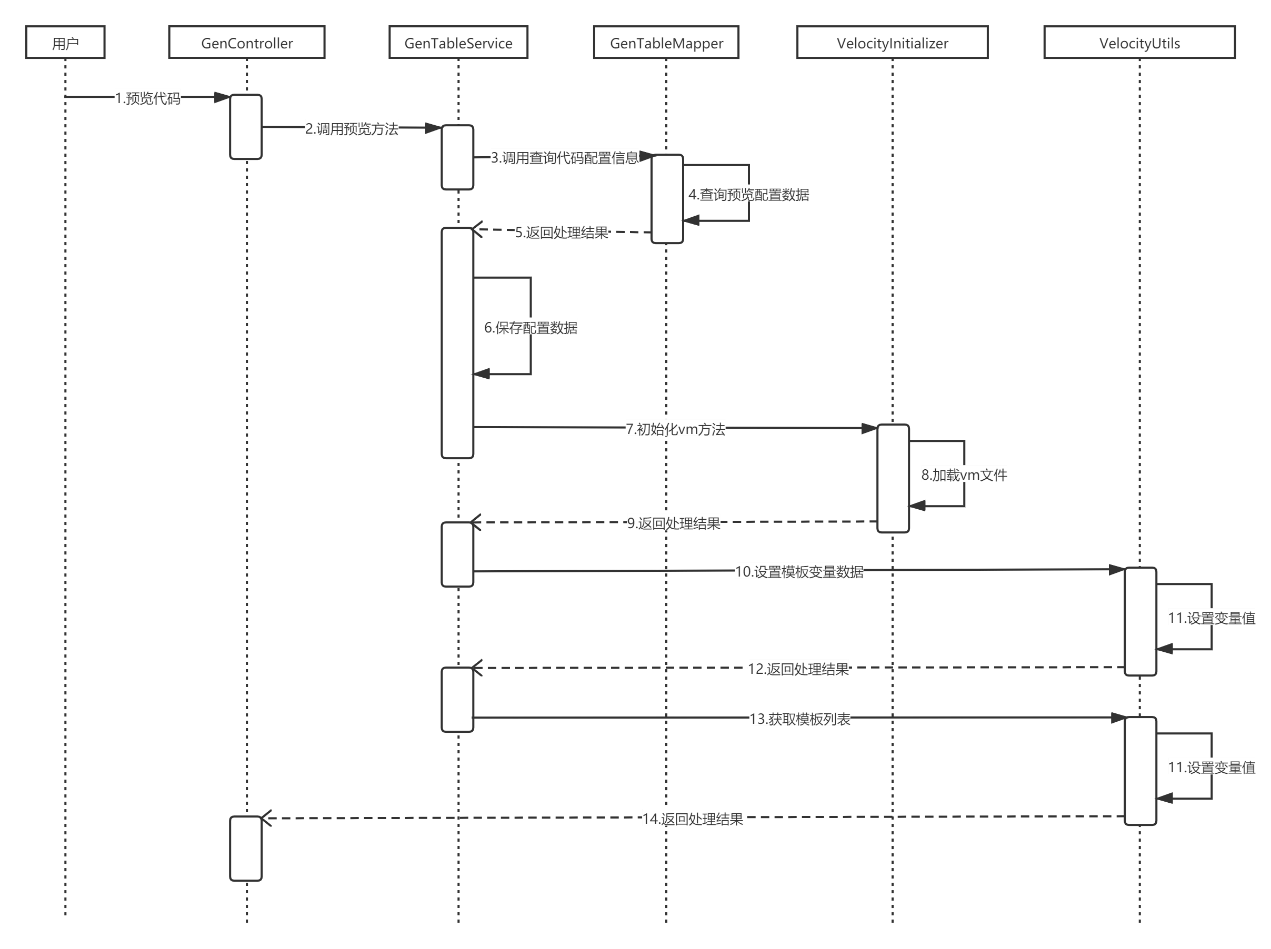
\includegraphics[width=0.8\textwidth]{figures/fig4-10.png}
  \caption{代码预览功能时序图}
  \label{fig4-10}
\end{figure}

\subsection{数据同步功能}
用户在修改已导入的数据表后需要点击数据同步按钮才能将修改后的表结构同步到当前配置中。点击数据同步时，平台会调用 GenController 中的接口，然后通过调用 GenTableMapper 中的查询配置数据方法查询配置信息，完成后调用 GenTableColumnMapper 中的方法查询被修改的数据表信息。

{\sloppy 根据查询的数据表数据调用 GenUtils 工具类中的初始化列属性方法，完成后调用 StringUtils 对相应的 Java 字段进行初始化设置。完成初始化设置后根据需要调用新增表的业务字段信息数据，随后删除原字段信息数据。如图 \ref{fig4-11} 所示。\par}

\begin{figure}[H]
  \centering
  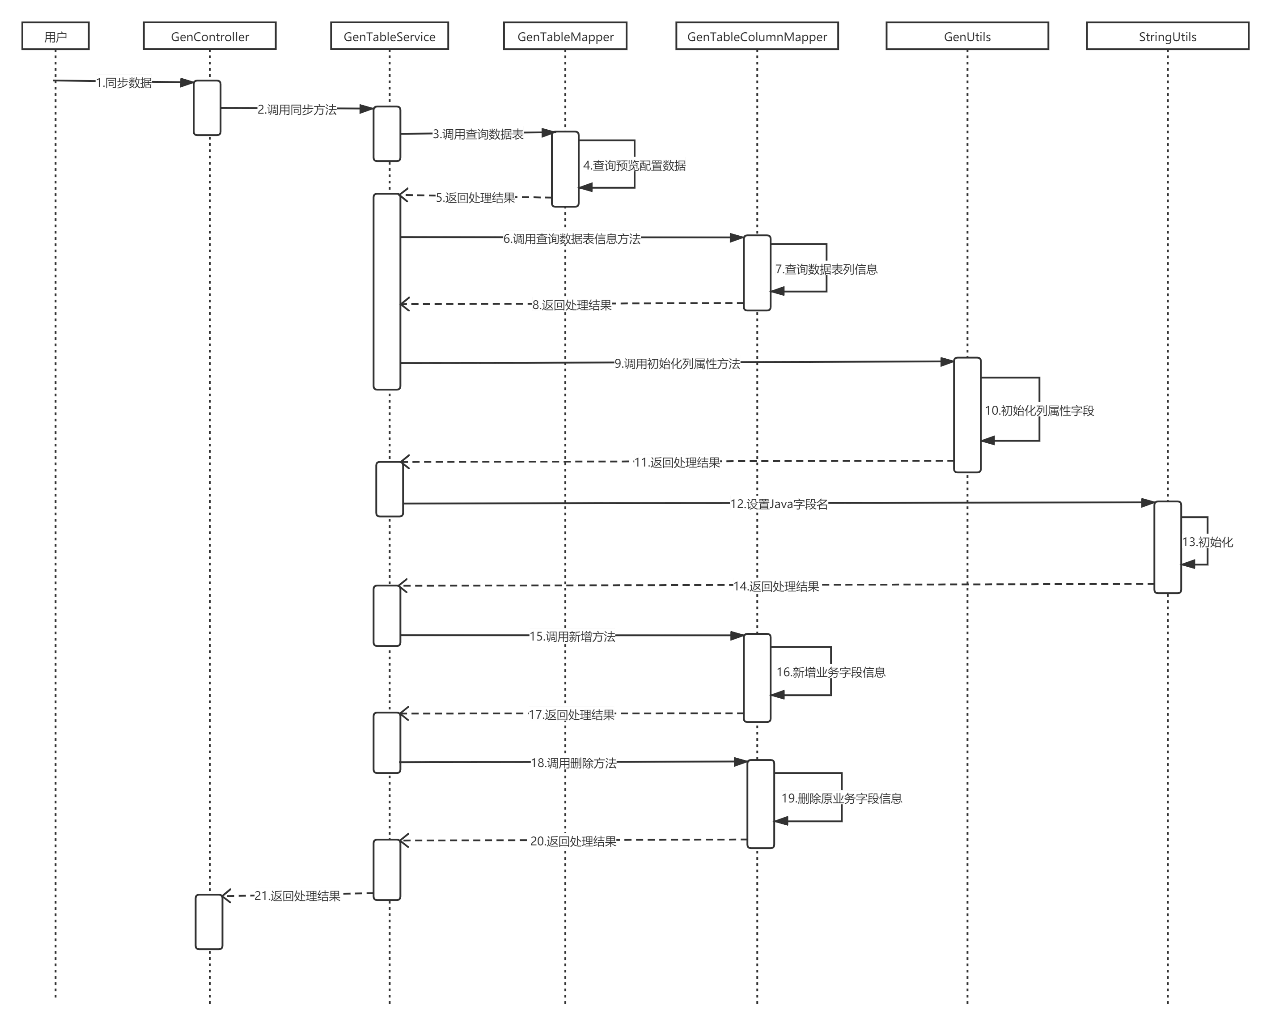
\includegraphics[width=0.8\textwidth]{figures/fig4-11.png}
  \caption{数据同步功能时序图}
  \label{fig4-11}
\end{figure}

\subsection{代码生成功能}
用户点击生成按钮后系统会根据配置调用不同的生成方式。

当选择生成压缩包时，后端调用 GenTableService 中查询数据表信息并生成代码的功能，然后查询生成表的信息，根据返回数据动态设置主键列信息。完成数据配置后初始化 vm 模板，然后调用 VelocityUtils 中的设置模板变量信息方法进行处理，完成模板配置后再调用添加模板信息方法。平台完成代码生成后会将所有文件按配置路径保存并设置文件名，并调用 VelocityInitializer 中的打包方法将生成的文件打成压缩包并下载。

当用户选择自定义路径下载时，生成文件步骤同生成压缩包，只是在生成文件后会将文件下载到用户自定义路径。如图 \ref{fig4-12} 所示。

\begin{figure}[H]
  \centering
  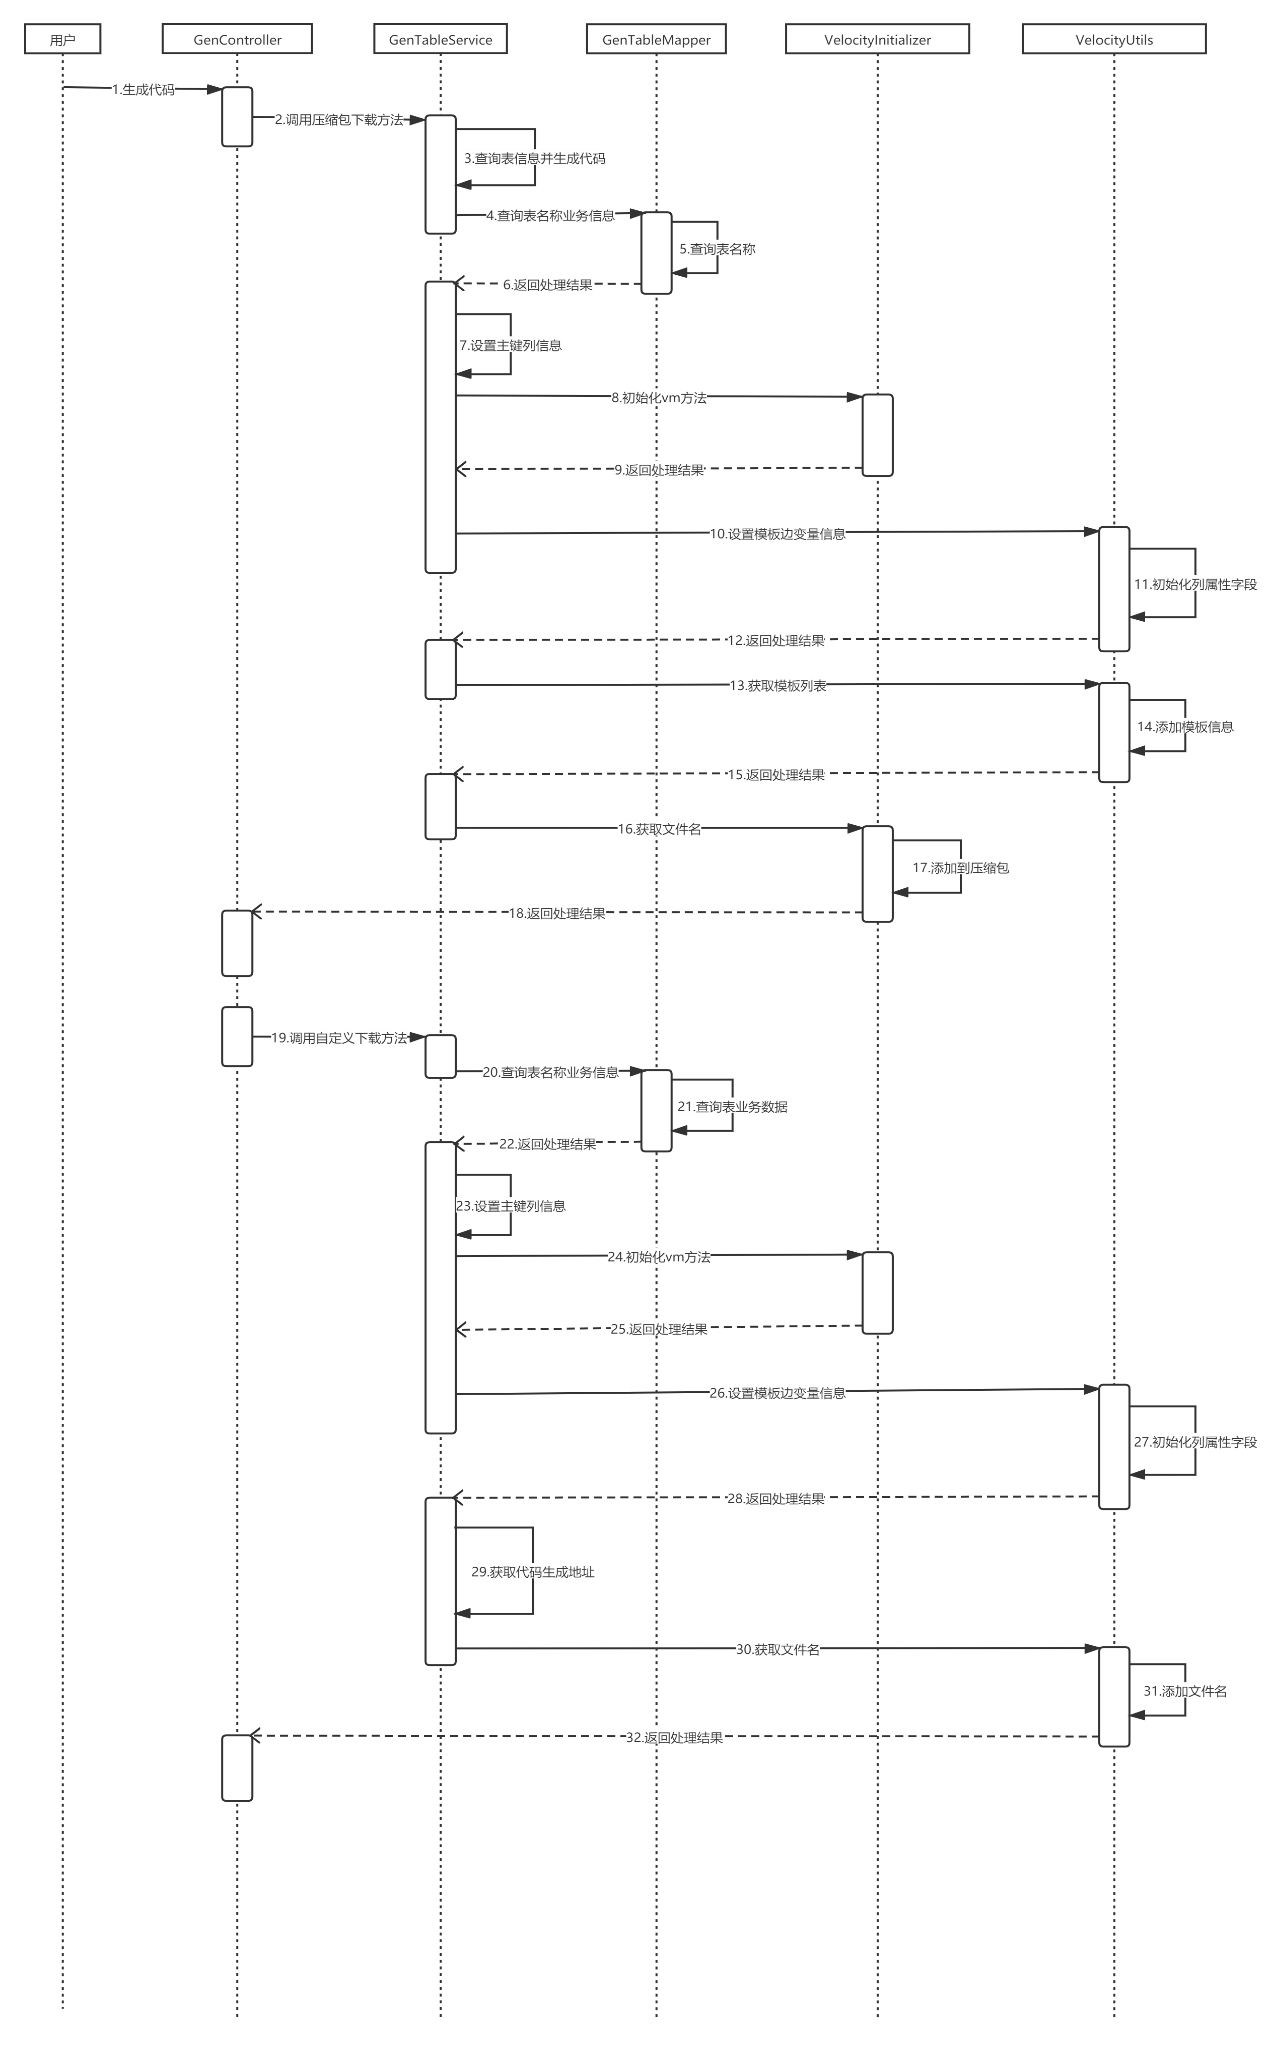
\includegraphics[height=0.82\textheight]{figures/fig4-12.png}
  \caption{代码生成功能时序图}
  \label{fig4-12}
\end{figure}

\subsection{组件拖拽功能}
用户进入构建页面后，可通过点击或拖拽组件构建页面。当用户点击或拖拽组件时，通过调用 CloneComponent 方法来复制选中组件，并随鼠标移动（按住鼠标左键）。当用户在构建区释放鼠标左键，执行 AddComponent 方法则将该组件添加到页面数组中。如图 \ref{fig4-13} 所示。

\begin{figure}[H]
  \centering
  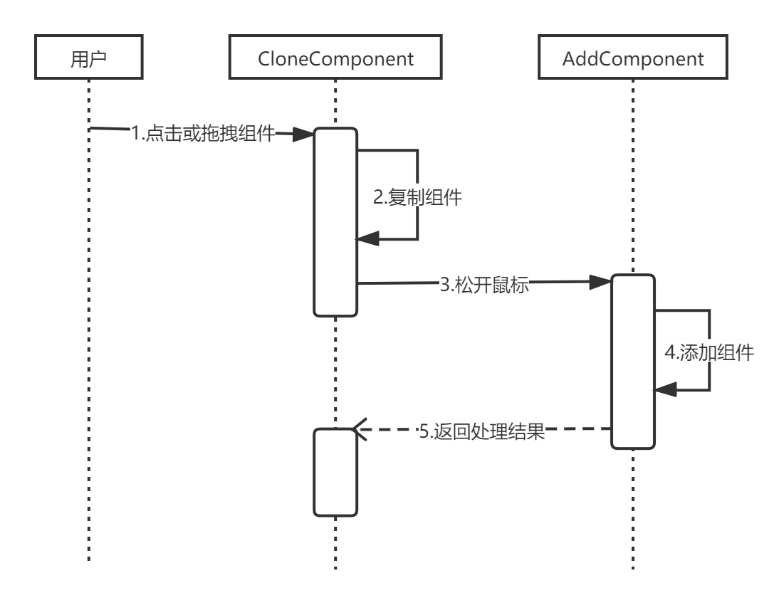
\includegraphics[width=0.65\textwidth]{figures/fig4-13.png}
  \caption{组件拖拽功能时序图}
  \label{fig4-13}
\end{figure}

\subsection{组件属性编辑功能}
用户在构建页面时能够对已选择的组件属性进行编辑。用户可通过点击组件右上角的复制（Append）按钮在该组件后复制一个完全相同的组件，也可通过点击右上角的删除（Remove）按钮删除当前组件。

用户通过鼠标左键点击组件时，在菜单右侧属性框中展示该组件属性（组件名、组件大小、栅格数、正则验证等）。用户可通过 TagChange、SetTimeValue、AddNode 等方法编辑这些属性，从而完成对组件的详细配置。如图 \ref{fig4-14} 所示。

\begin{figure}[H]
  \centering
  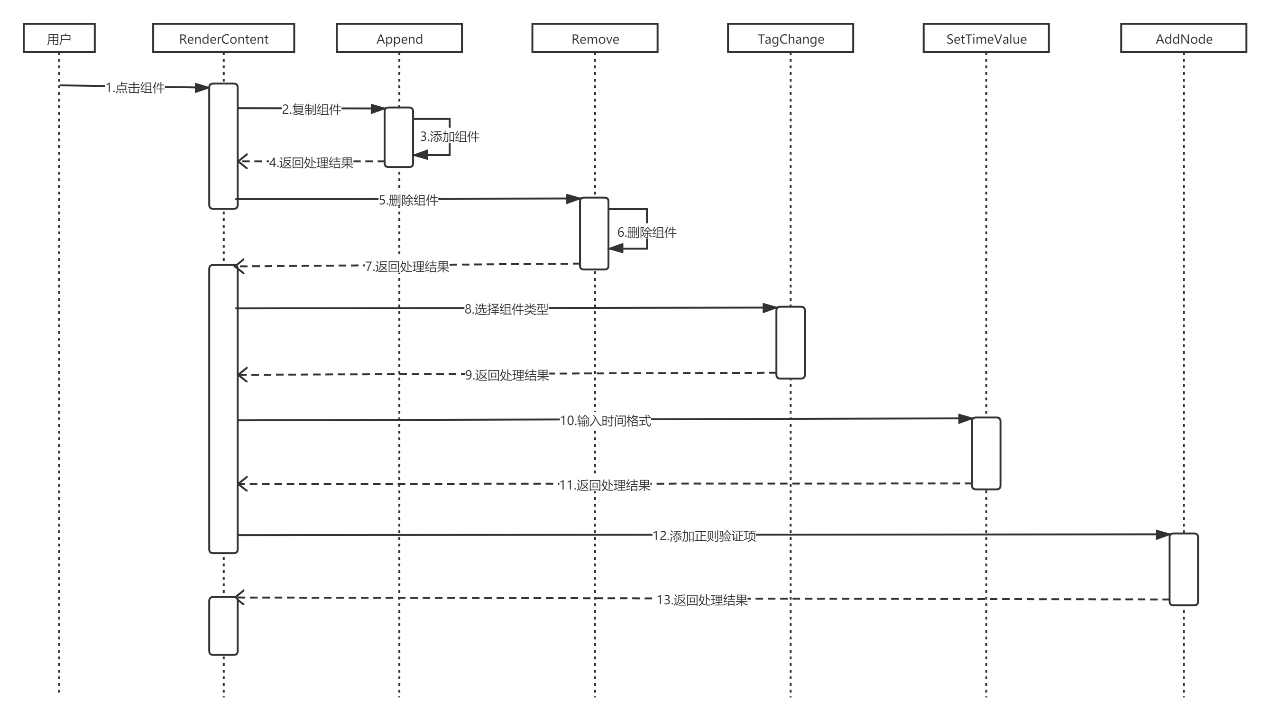
\includegraphics[width=0.8\textwidth]{figures/fig4-14.png}
  \caption{组件属性编辑功能时序图}
  \label{fig4-14}
\end{figure}

\subsection{页面属性编辑功能}
用户在平台右侧选择页面属性后，可对构建页面的属性进行编辑。用户可通过 RenderContent 方法对页面的大小、对齐方式等属性进行编辑。

在完成页面构建后通过点击编辑区上方的导出文件按钮，便可下载用户构建的页面文件，导出时可选择页面或弹窗。

用户同样可以通过直接点击复制代码来复制构建页面的代码，通过 Copy 方法将复制内容存入用户操作系统剪切板内。当用户不满意时，可点击清空按钮直接清空编辑区所有组件。如图 \ref{fig4-15} 所示。

\begin{figure}[H]
  \centering
  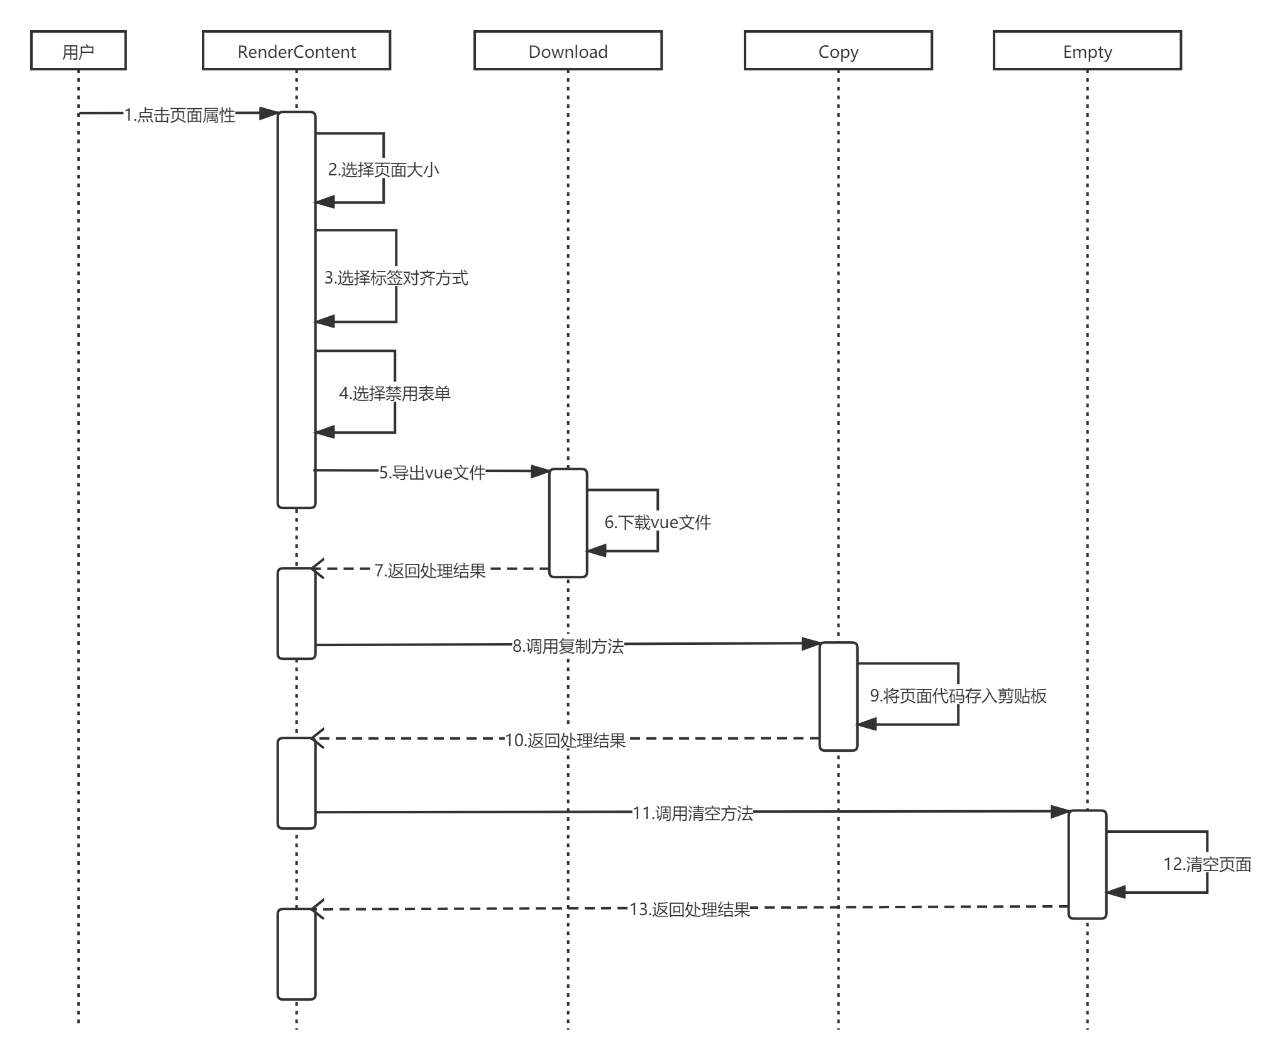
\includegraphics[width=0.75\textwidth]{figures/fig4-15.png}
  \caption{页面属性编辑功能时序图}
  \label{fig4-15}
\end{figure}

\subsection{在线预览功能}
用户在构建页面的过程中，可随时通过点击运行按钮预览已构建部分。用户点击运行（Run）后，通过在线编译器编译页面代码，在预览页面左侧展示编译后的全部页面代码，在右侧展示编译页面。用户能够直接对页面进行操作，测试构建页面功能。如图 \ref{fig4-16} 所示。

\begin{figure}[H]
  \centering
  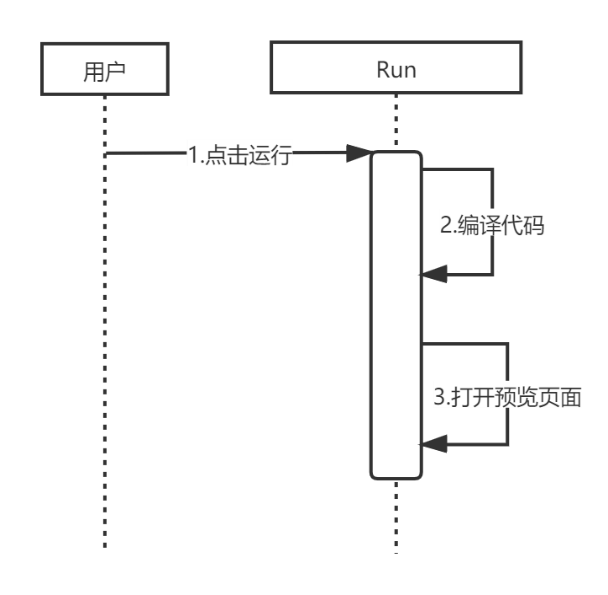
\includegraphics[width=0.55\textwidth]{figures/fig4-16.png}
  \caption{在线预览功能时序图}
  \label{fig4-16}
\end{figure}

\subsection{界面模板功能}
用户在完成构建页面后可分享该页面。用户进入界面模板页后，系统通过调用 TemplateMapper 中的查询方法查询所有模板列表，并展示出来。

用户点击分享按钮后，平台先将该页面文件上传至服务器，然后请求后端 TemplateController 中的分享接口，以及调用 TemplateMapper 中的新增方法将用户 id、文件地址插入界面模板数据表中。

用户删除模板时先判断当前模板是否是该用户发布的，确定后调用 TemplateMapper 中的 delete 方法删除数据表中相应字段并根据文件路径删除服务器中的文件。

分享后的界面可供所有本平台用户下载，点击下载时直接获取当前文件的路径，随后拉起浏览器请求进行下载。如图 \ref{fig4-17} 所示。

\begin{figure}[H]
  \centering
  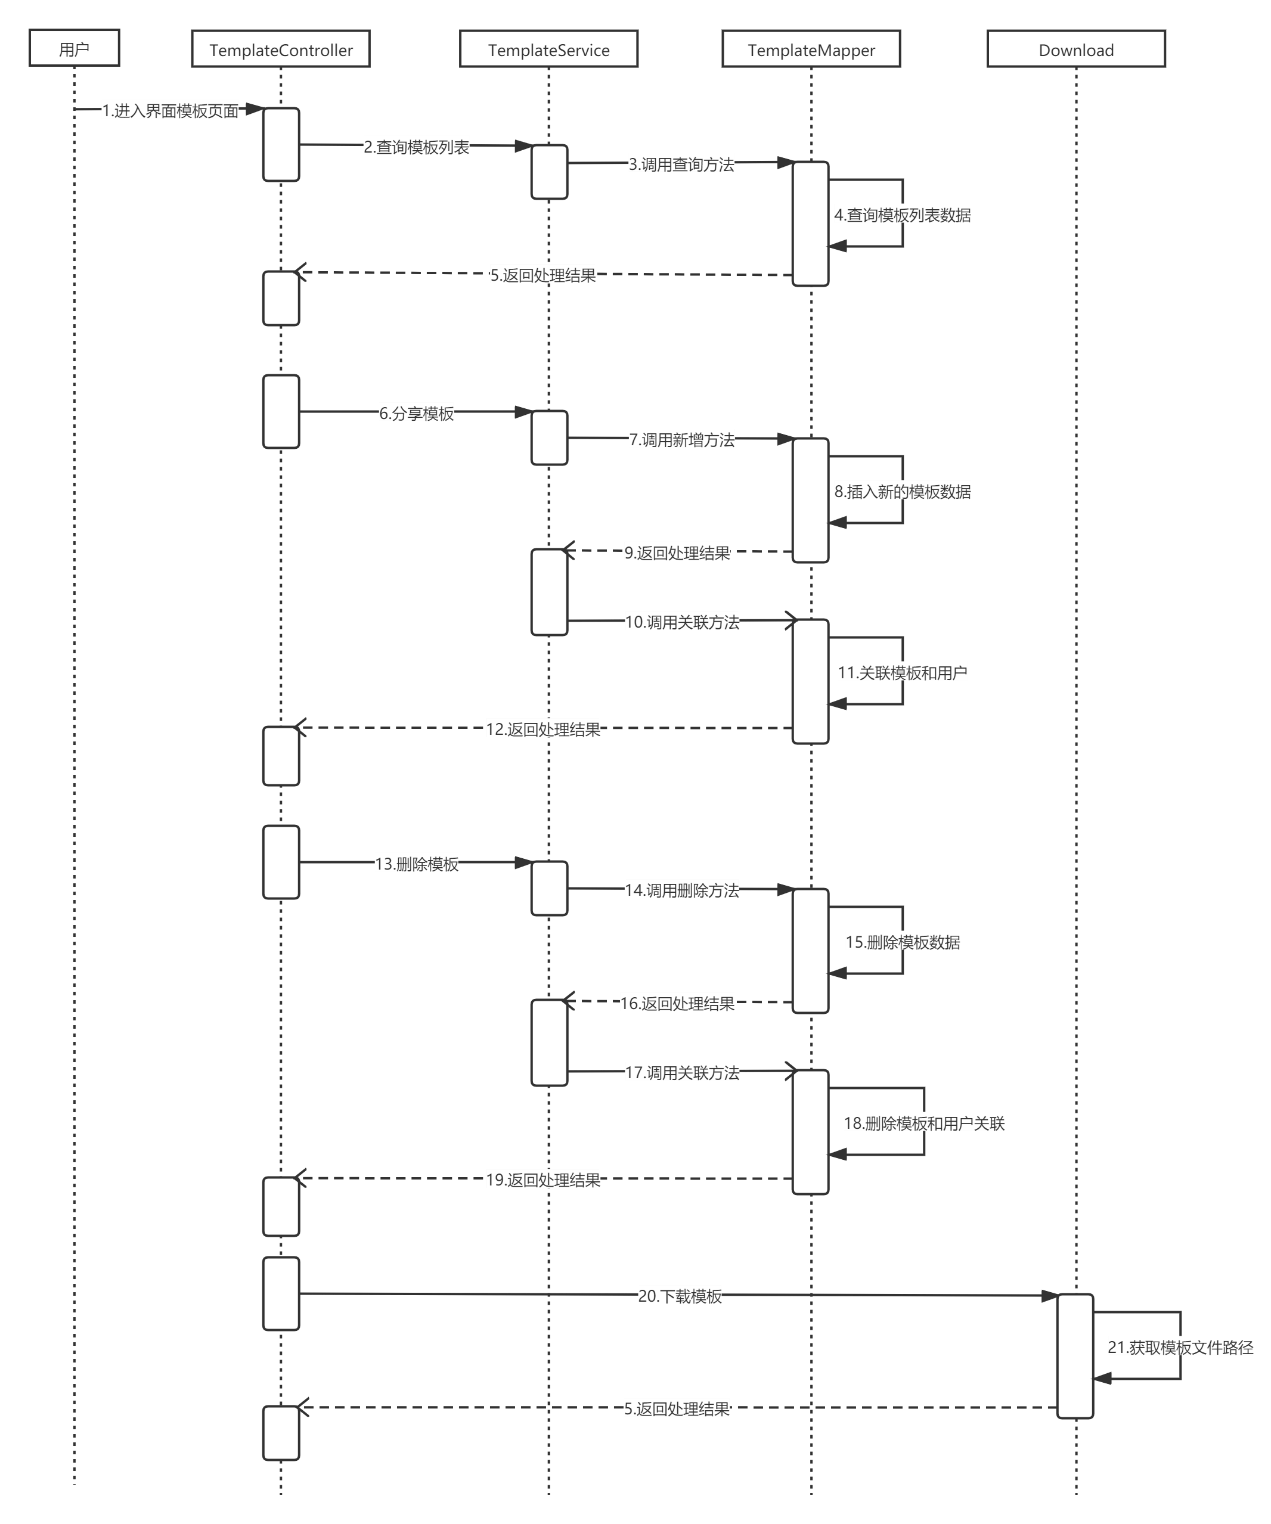
\includegraphics[height=0.82\textheight]{figures/fig4-17.png}
  \caption{界面模板功能时序图}
  \label{fig4-17}
\end{figure}

\section{数据库设计}

\subsection{总体设计}
根据系统功能性需求分析，对系统数据表进行了总体设计，并形成 E-R 图（图中实体仅展示部分字段）。

用户在登录时会产生登录日志，一个用户可对应多条登录日志表数据。管理员在新增用户后可根据需求为用户分配相应角色，一个用户可同时具有多个角色，一个角色也能同时分配给多个用户。管理员可以通过给角色配置菜单来实现角色权限设置，一个角色可设置多个菜单，而一个菜单项也可以对应多个角色。操作日志表用来记录用户在平台中的操作，一个角色对应多条操作记录。管理员每次新建系统参数后会产生一条系统参数配置数据，因此一个用户对应多个参数数据。

用户在创建每一张数据表后会产生一条对该表信息进行记录的数据，将该表导入代码生成业务表后，代码生成业务表和代码生成业务字段表会相应地新增一条针对该表生成代码配置的数据。用户在编辑生成代码配置时可选择表字段的数据字典类型，在生成代码后对应字段会根据字典类型自动匹配字典数据。

用户在完成页面构建后，可将其模板进行分享，这时系统会保存其页面文件并将该页面文件的地址、该用户 id 存入界面模板表。如图 \ref{fig4-18} 所示。

\begin{figure}[H]
  \centering
  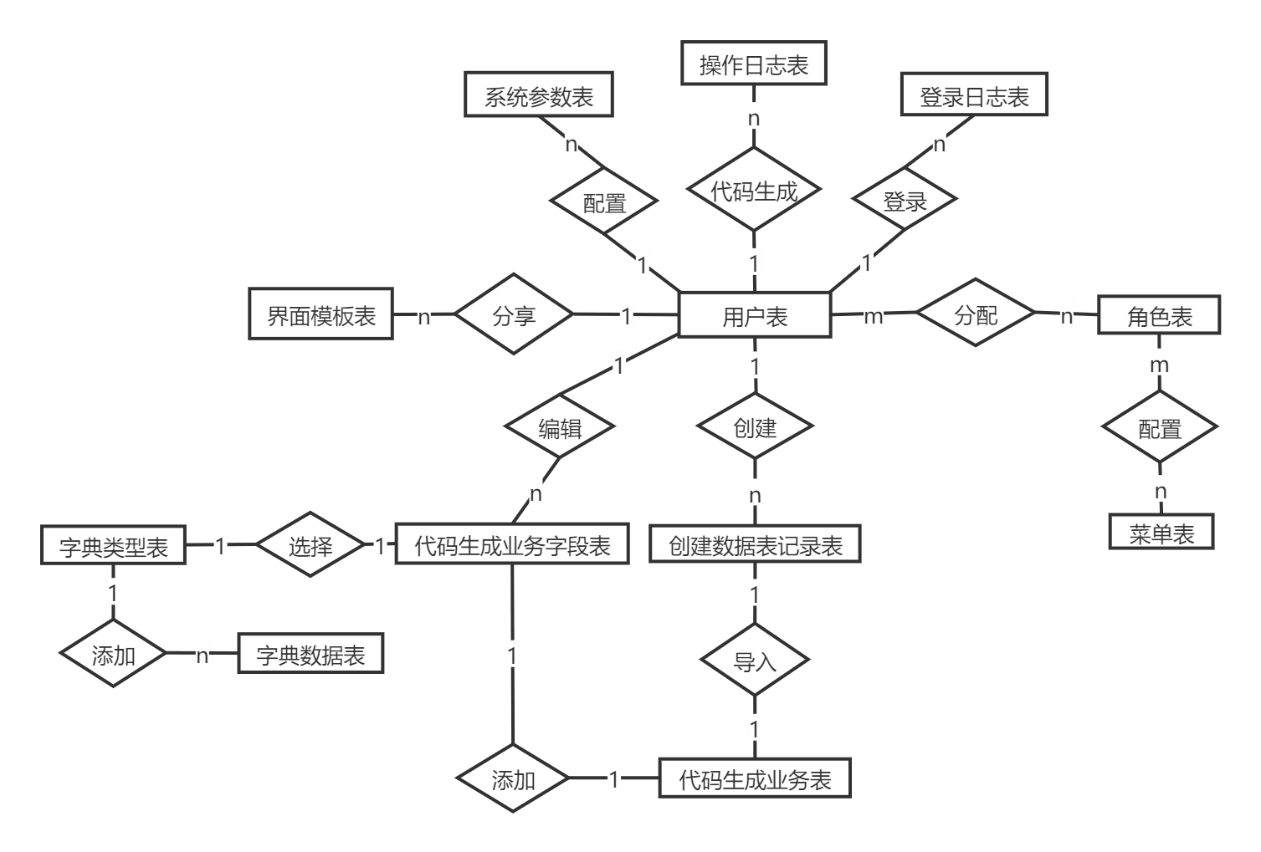
\includegraphics[width=0.95\textwidth]{figures/fig4-18.png}
  \caption{数据库总体设计 E-R 图}
  \label{fig4-18}
\end{figure}

\subsection{数据库表设计}

\subsubsection{用户表（sys\_user）}
用户表存储所有的系统用户数据，其中包含用户 id、用户名、用户密码、用户角色 id 等 18 个字段。见表 \ref{tab4-1}。

\begin{table}[H]
  \centering
  \caption{用户表}
  \label{tab4-1}
  \zihao{5}\songti
  \begin{tabular}{c l l l p{4.5cm}}
    \toprule
    序号 & 英文字段名 & 中文字段名 & 字段类型 & 备注 \\
    \midrule
    1 & user\_id & 用户 ID & bigint(20) & 用户 ID \\
    2 & user\_name & 用户账号 & varchar(30) & 用户账号 \\
    3 & nick\_name & 用户昵称 & varchar(30) & 用户昵称 \\
    4 & user\_type & 用户类型 & varchar(2) & 用户类型（00 系统用户） \\
    5 & email & 用户邮箱 & varchar(50) & 用户邮箱 \\
    6 & phonenumber & 手机号码 & varchar(11) & 手机号码 \\
    7 & sex & 用户性别 & char(1) & 用户性别（0 男 1 女 2 未知） \\
    8 & avatar & 头像地址 & varchar(100) & 头像地址 \\
    9 & password & 密码 & varchar(100) & 密码 \\
    10 & status & 帐号状态 & char(1) & 帐号状态（0 正常 1 停用） \\
    11 & del\_flag & 删除标志 & char(1) & 删除标志（0 代表存在 2 代表删除） \\
    12 & login\_ip & 最后登录 IP & varchar(50) & 最后登录 IP \\
    13 & login\_date & 最后登录时间 & datetime & 最后登录时间 \\
    14 & create\_by & 创建者 & varchar(64) & 创建者 \\
    15 & create\_time & 创建时间 & datetime & 创建时间 \\
    16 & update\_by & 更新者 & varchar(64) & 更新者 \\
    17 & update\_time & 更新时间 & datetime & 更新时间 \\
    18 & remark & 备注 & varchar(500) & 备注 \\
    \bottomrule
  \end{tabular}
\end{table}

\subsubsection{角色表（sys\_role）}
角色表存储包括管理员在内的所有系统角色，其中包含角色 id、角色名称、角色权限、角色状态等 12 个字段。见表 \ref{tab4-2}。

\begin{table}[H]
  \centering
  \caption{角色表}
  \label{tab4-2}
  \zihao{5}\songti
  \begin{tabular}{c l l l p{4.5cm}}
    \toprule
    序号 & 英文字段名 & 中文字段名 & 字段类型 & 备注 \\
    \midrule
    1 & role\_id & 角色 ID & bigint(20) & 角色 ID \\
    2 & role\_name & 角色名称 & varchar(30) & 角色名称 \\
    3 & role\_key & 角色权限字符串 & varchar(100) & 角色权限字符串 \\
    4 & role\_sort & 显示顺序 & int(4) & 显示顺序 \\
    5 & menu\_check\_strictly & 菜单树选择项是否关联显示 & tinyint(1) & 菜单树选择项是否关联显示 \\
    6 & status & 角色状态 & char(1) & 角色状态（0 正常 1 停用） \\
    7 & del\_flag & 删除标志 & char(1) & 删除标志（0 代表存在 2 代表删除） \\
    8 & create\_by & 创建者 & varchar(64) & 创建者 \\
    9 & create\_time & 创建时间 & datetime & 创建时间 \\
    10 & update\_by & 更新者 & varchar(64) & 更新者 \\
    11 & update\_time & 更新时间 & datetime & 更新时间 \\
    12 & remark & 备注 & varchar(500) & 备注 \\
    \bottomrule
  \end{tabular}
\end{table}

\subsubsection{用户角色关联表（sys\_role\_user）}
角色用户关联表主要用来存储用户 id 和角色 id，共 2 个字段。见表 \ref{tab4-3}。

\begin{table}[H]
  \centering
  \caption{用户角色关联表}
  \label{tab4-3}
  \zihao{5}\songti
  \begin{tabular}{c l l l l}
    \toprule
    序号 & 英文字段名 & 中文字段名 & 字段类型 & 备注 \\
    \midrule
    1 & user\_id & 用户 ID & bigint(20) & 用户 ID \\
    2 & role\_id & 角色 ID & bigint(20) & 角色 ID \\
    \bottomrule
  \end{tabular}
\end{table}

\subsubsection{菜单表（sys\_menu）}
菜单表存储所有的系统菜单数据，其中包含菜单 id、菜单名称、父菜单 id、菜单路径等 18 个字段。见表 \ref{tab4-4}。

\begin{table}[H]
  \centering
  \caption{菜单表}
  \label{tab4-4}
  \zihao{5}\songti
  \begin{tabular}{c l l l p{4.5cm}}
    \toprule
    序号 & 英文字段名 & 中文字段名 & 字段类型 & 备注 \\
    \midrule
    1 & menu\_id & 菜单 ID & bigint(20) & 菜单 ID \\
    2 & menu\_name & 菜单名称 & varchar(50) & 菜单名称 \\
    3 & parent\_id & 父菜单 ID & bigint(20) & 父菜单 ID \\
    4 & order\_num & 显示顺序 & int(4) & 显示顺序 \\
    5 & path & 路由地址 & varchar(200) & 路由地址 \\
    6 & component & 组件路径 & varchar(255) & 组件路径 \\
    7 & is\_frame & 是否为外链 & int(1) & 是否为外链（0 是 1 否） \\
    8 & is\_cache & 是否缓存 & int(1) & 是否缓存（0 缓存 1 不缓存） \\
    9 & menu\_type & 菜单类型 & char(1) & 菜单类型（M 目录 C 菜单 F 按钮） \\
    10 & visible & 菜单状态 & char(1) & 菜单状态（0 显示 1 隐藏） \\
    11 & status & 菜单状态 & char(1) & 菜单状态（0 正常 1 停用） \\
    12 & perms & 权限标识 & varchar(100) & 权限标识 \\
    13 & icon & 菜单图标 & varchar(100) & 菜单图标 \\
    14 & create\_by & 创建者 & varchar(64) & 创建者 \\
    15 & create\_time & 创建时间 & datetime & 创建时间 \\
    16 & update\_by & 更新者 & varchar(64) & 更新者 \\
    17 & update\_time & 更新时间 & datetime & 更新时间 \\
    18 & remark & 备注 & varchar(500) & 备注 \\
    \bottomrule
  \end{tabular}
\end{table}

\subsubsection{角色菜单关联表（sys\_role\_menu）}
角色菜单关联表主要包括菜单 id 和角色 id，共 2 个字段。见表 \ref{tab4-5}。

\begin{table}[H]
  \centering
  \caption{角色菜单关联表}
  \label{tab4-5}
  \zihao{5}\songti
  \begin{tabular}{c l l l l}
    \toprule
    序号 & 英文字段名 & 中文字段名 & 字段类型 & 备注 \\
    \midrule
    1 & role\_id & 角色 ID & bigint(20) & 角色 ID \\
    2 & menu\_id & 菜单 ID & bigint(20) & 菜单 ID \\
    \bottomrule
  \end{tabular}
\end{table}

\subsubsection{系统参数表（sys\_config）}
系统参数表包括参数主键、参数名称、参数键值、系统内置等 10 个字段。见表 \ref{tab4-6}。

\begin{table}[H]
  \centering
  \caption{系统参数表}
  \label{tab4-6}
  \zihao{5}\songti
  \begin{tabular}{c l l l p{4cm}}
    \toprule
    序号 & 英文字段名 & 中文字段名 & 字段类型 & 备注 \\
    \midrule
    1 & config\_id & 参数主键 & int(5) & 参数主键 \\
    2 & config\_name & 参数名称 & varchar(100) & 参数名称 \\
    3 & config\_key & 参数键名 & varchar(100) & 参数键名 \\
    4 & config\_value & 参数键值 & varchar(500) & 参数键值 \\
    5 & config\_type & 系统内置 & char(1) & 系统内置（Y 是 N 否） \\
    6 & create\_by & 创建者 & varchar(64) & 创建者 \\
    7 & create\_time & 创建时间 & datetime & 创建时间 \\
    8 & update\_by & 更新者 & varchar(64) & 更新者 \\
    9 & update\_time & 更新时间 & datetime & 更新时间 \\
    10 & remark & 备注 & varchar(500) & 备注 \\
    \bottomrule
  \end{tabular}
\end{table}

\subsubsection{登录日志表（sys\_logininfor）}
登录日志表包括访问 id、用户账号、登录 IP 地址、登录状态、提示信息、访问时间，共 6 个字段。见表 \ref{tab4-7}。

\begin{table}[H]
  \centering
  \caption{登录日志表}
  \label{tab4-7}
  \zihao{5}\songti
  \begin{tabular}{c l l l p{4cm}}
    \toprule
    序号 & 英文字段名 & 中文字段名 & 字段类型 & 备注 \\
    \midrule
    1 & info\_id & 访问 ID & bigint(20) & 访问 ID \\
    2 & user\_name & 用户账号 & varchar(50) & 用户账号 \\
    3 & ipaddr & 登录 IP 地址 & varchar(50) & 登录 IP 地址 \\
    4 & status & 登录状态 & char(1) & 登录状态（0 成功 1 失败） \\
    5 & msg & 提示信息 & varchar(255) & 提示信息 \\
    6 & access\_time & 访问时间 & datetime & 访问时间 \\
    \bottomrule
  \end{tabular}
\end{table}

\subsubsection{操作日志表（sys\_oper\_log）}
操作日志表包含日志 id、业务名称、方法名称、操作类别、操作状态等 15 个字段。见表 \ref{tab4-8}。

\begin{table}[H]
  \centering
  \caption{操作日志表}
  \label{tab4-8}
  \zihao{5}\songti
  \begin{tabular}{c l l l p{4.5cm}}
    \toprule
    序号 & 英文字段名 & 中文字段名 & 字段类型 & 备注 \\
    \midrule
    1 & oper\_id & 日志主键 & bigint(20) & 日志主键 \\
    2 & title & 模块标题 & varchar(50) & 模块标题 \\
    3 & business\_type & 业务类型 & int(2) & 业务类型（0 其它 1 新增 2 修改 3 删除） \\
    4 & method & 方法名称 & varchar(100) & 方法名称 \\
    5 & request\_method & 请求方式 & varchar(10) & 请求方式 \\
    6 & operator\_type & 操作类别 & int(1) & 操作类别（0 其它 1 后台用户 2 手机端用户） \\
    7 & oper\_name & 操作人员 & varchar(50) & 操作人员 \\
    8 & oper\_url & 请求 URL & varchar(255) & 请求 URL \\
    9 & oper\_ip & 主机地址 & varchar(50) & 主机地址 \\
    10 & oper\_location & 操作地点 & varchar(255) & 操作地点 \\
    11 & oper\_param & 请求参数 & varchar(2000) & 请求参数 \\
    12 & json\_result & 返回参数 & varchar(2000) & 返回参数 \\
    13 & status & 操作状态 & int(1) & 操作状态（0 正常 1 异常） \\
    14 & error\_msg & 错误消息 & varchar(2000) & 错误消息 \\
    15 & oper\_time & 操作时间 & datetime & 操作时间 \\
    \bottomrule
  \end{tabular}
\end{table}

\subsubsection{字典类型表（sys\_dict\_type）}
字典类型表包括含典 id，字典名称、字典类型、状态、创建者等 9 个字段。见表 \ref{tab4-9}。

\begin{table}[H]
  \centering
  \caption{字典类型表}
  \label{tab4-9}
  \zihao{5}\songti
  \begin{tabular}{c l l l p{4cm}}
    \toprule
    序号 & 英文字段名 & 中文字段名 & 字段类型 & 备注 \\
    \midrule
    1 & dict\_id & 字典主键 & bigint(20) & 字典主键 \\
    2 & dict\_name & 字典名称 & varchar(100) & 字典名称 \\
    3 & dict\_type & 字典类型 & varchar(100) & 字典类型 \\
    4 & status & 状态 & char(1) & 状态（0 正常 1 停用） \\
    5 & create\_by & 创建者 & varchar(64) & 创建者 \\
    6 & create\_time & 创建时间 & datetime & 创建时间 \\
    7 & update\_by & 更新者 & varchar(64) & 更新者 \\
    8 & update\_time & 更新时间 & datetime & 更新时间 \\
    9 & remark & 备注 & varchar(500) & 备注 \\
    \bottomrule
  \end{tabular}
\end{table}

\subsubsection{字典数据表（sys\_dict\_data）}
字典数据表包含字典编码、字典键值、字典类型、样式属性等 14 个字段。见表 \ref{tab4-10}。

\begin{table}[H]
  \centering
  \caption{字典数据表}
  \label{tab4-10}
  \zihao{5}\songti
  \begin{tabular}{c l l l p{4cm}}
    \toprule
    序号 & 英文字段名 & 中文字段名 & 字段类型 & 备注 \\
    \midrule
    1 & dict\_code & 字典编码 & bigint(20) & 字典编码 \\
    2 & dict\_sort & 字典排序 & int(4) & 字典排序 \\
    3 & dict\_label & 字典标签 & varchar(100) & 字典标签 \\
    4 & dict\_value & 字典键值 & varchar(100) & 字典键值 \\
    5 & dict\_type & 字典类型 & varchar(100) & 字典类型 \\
    6 & css\_class & 样式属性 & varchar(100) & 样式属性（其他样式扩展） \\
    7 & list\_class & 表格回显样式 & varchar(100) & 表格回显样式 \\
    8 & is\_default & 是否默认 & char(1) & 是否默认（Y 是 N 否） \\
    9 & status & 状态 & char(1) & 状态（0 正常 1 停用） \\
    10 & create\_by & 创建者 & varchar(64) & 创建者 \\
    11 & create\_time & 创建时间 & datetime & 创建时间 \\
    12 & update\_by & 更新者 & varchar(64) & 更新者 \\
    13 & update\_time & 更新时间 & datetime & 更新时间 \\
    14 & remark & 备注 & varchar(500) & 备注 \\
    \bottomrule
  \end{tabular}
\end{table}

\subsubsection{用户代码生成关联表（sys\_user\_gen\_table）}
用户代码生成关联表包含用户 id 和代码生成表 id，共 2 个字段。见表 \ref{tab4-11}。

\begin{table}[H]
  \centering
  \caption{用户代码生成关联表}
  \label{tab4-11}
  \zihao{5}\songti
  \begin{tabular}{c l l l l}
    \toprule
    序号 & 英文字段名 & 中文字段名 & 字段类型 & 备注 \\
    \midrule
    1 & table\_id & 代码生成表 id & bigint(20) & 代码生成表 id \\
    2 & user\_id & 用户 id & bigint(20) & 用户 id \\
    \bottomrule
  \end{tabular}
\end{table}

\subsubsection{创建数据表记录表}
创建数据表记录表主要用来记录用户创建的全部记录，表中包含主键 id、数据表名和用户 id 共 3 个字段。见表 \ref{tab4-12}。

\begin{table}[H]
  \centering
  \caption{创建数据表记录表}
  \label{tab4-12}
  \zihao{5}\songti
  \begin{tabular}{c l l l l}
    \toprule
    序号 & 英文字段名 & 中文字段名 & 字段类型 & 备注 \\
    \midrule
    1 & business\_id & 主键 id & bigint(20) & 主键 id \\
    2 & table\_name & 创建表名 & varchar(50) & 创建表名 \\
    3 & user\_id & 用户 id & bigint(20) & 用户 id \\
    \bottomrule
  \end{tabular}
\end{table}

\subsubsection{代码生成表（gen\_table）}
代码生成表包含编号（主键 id）、表名称、表描述、生成代码方式等 18 个字段。见表 \ref{tab4-13}。

\begin{table}[H]
  \centering
  \caption{代码生成表}
  \label{tab4-13}
  \zihao{5}\songti
  \begin{tabular}{c l l l p{4.5cm}}
    \toprule
    序号 & 英文字段名 & 中文字段名 & 字段类型 & 备注 \\
    \midrule
    1 & table\_id & 编号 & bigint(20) & 编号 \\
    2 & table\_name & 表名称 & varchar(200) & 表名称 \\
    3 & table\_comment & 表描述 & varchar(500) & 表描述 \\
    4 & class\_name & 实体类名称 & varchar(100) & 实体类名称 \\
    5 & tpl\_category & 使用的模板 & varchar(200) & 使用的模板（crud 单表操作 tree 树表操作） \\
    6 & package\_name & 生成包路径 & varchar(100) & 生成包路径 \\
    7 & module\_name & 生成模块名 & varchar(30) & 生成模块名 \\
    8 & business\_name & 生成业务名 & varchar(30) & 生成业务名 \\
    9 & function\_name & 生成功能名 & varchar(50) & 生成功能名 \\
    10 & function\_author & 生成功能作者 & varchar(50) & 生成功能作者 \\
    11 & gen\_type & 生成代码方式 & char(1) & 生成代码方式（0zip 压缩包 1 自定义路径） \\
    12 & gen\_path & 生成路径 & varchar(200) & 生成路径（不填默认项目路径） \\
    13 & options & 其它生成选项 & varchar(1000) & 其它生成选项 \\
    14 & create\_by & 创建者 & varchar(64) & 创建者 \\
    15 & create\_time & 创建时间 & datetime & 创建时间 \\
    16 & update\_by & 更新者 & varchar(64) & 更新者 \\
    17 & update\_time & 更新时间 & datetime & 更新时间 \\
    18 & remark & 备注 & varchar(500) & 备注 \\
    \bottomrule
  \end{tabular}
\end{table}

\subsubsection{代码生成字段表（gen\_table\_column）}
代码生成表包含编号（主键 id）、归属表编号、列名称、Java 字段名等 22 个字段。见表 \ref{tab4-14}。

\begin{table}[H]
  \centering
  \caption{代码生成字段表}
  \label{tab4-14}
  \zihao{5}\songti
  \begin{tabular}{c l l l p{4.5cm}}
    \toprule
    序号 & 英文字段名 & 中文字段名 & 字段类型 & 备注 \\
    \midrule
    1 & column\_id & 编号 & bigint(20) & 编号 \\
    2 & table\_id & 归属表编号 & varchar(64) & 归属表编号 \\
    3 & column\_name & 列名称 & varchar(200) & 列名称 \\
    4 & column\_comment & 列描述 & varchar(500) & 列描述 \\
    5 & column\_type & 列类型 & varchar(100) & 列类型 \\
    6 & java\_type & JAVA 类型 & varchar(500) & JAVA 类型 \\
    7 & java\_field & JAVA 字段名 & varchar(200) & JAVA 字段名 \\
    8 & is\_pk & 是否主键 & char(1) & 是否主键（1 是） \\
    9 & is\_increment & 是否自增 & char(1) & 是否自增（1 是） \\
    10 & is\_required & 是否必填 & char(1) & 是否必填（1 是） \\
    11 & is\_insert & 是否为插入字段 & char(1) & 是否为插入字段（1 是） \\
    12 & is\_edit & 是否编辑字段 & char(1) & 是否编辑字段（1 是） \\
    13 & is\_list & 是否列表字段 & char(1) & 是否列表字段（1 是） \\
    14 & is\_query & 是否查询字段 & char(1) & 是否查询字段（1 是） \\
    15 & query\_type & 查询方式 & varchar(200) & 查询方式（等于、不等于、大于、小于、范围） \\
    16 & html\_type & 显示类型 & varchar(200) & 显示类型（文本框、文本域、下拉框、复选框、单选框、日期控件） \\
    17 & dict\_type & 字典类型 & varchar(200) & 字典类型 \\
    18 & sort & 排序 & int(11) & 排序 \\
    19 & create\_by & 创建者 & varchar(64) & 创建者 \\
    20 & create\_time & 创建时间 & datetime & 创建时间 \\
    21 & update\_by & 更新者 & varchar(64) & 更新者 \\
    22 & update\_time & 更新时间 & datetime & 更新时间 \\
    \bottomrule
  \end{tabular}
\end{table}

\subsubsection{界面模板表（sys\_template）}
界面模板表包含模板 id、用户 id 和界面模板文件路径，共 3 个字段。见表 \ref{tab4-15}。

\begin{table}[H]
  \centering
  \caption{界面模板表}
  \label{tab4-15}
  \zihao{5}\songti
  \begin{tabular}{c l l l l}
    \toprule
    序号 & 英文字段名 & 中文字段名 & 字段类型 & 备注 \\
    \midrule
    1 & template\_id & 模板 id & bigint(20) & 模板 id \\
    2 & user\_id & 用户 id & bigint(20) & 用户 id \\
    3 & template\_url & 界面模板文件路径 & varchar(200) & 界面模板文件路径 \\
    \bottomrule
  \end{tabular}
\end{table}

\chapter{系统实现}

\section{登录功能}
用户通过统一的登录界面进行登录，如图 \ref{fig5-1} 所示。在用户输入用户名、密码、验证码登录时，平台会先校验验证码是否正确，如果正确则前往数据库根据用户名查询对应的密码，若存在该用户名且密码正确则完成登录；当出现验证码错误、用户名不存在、密码错误时，系统将给出相应提示。当用户名、密码、验证码都正确时平台会识别该用户角色的权限，然后根据该角色所具有的权限分配相应的系统资源给用户。

\begin{figure}[H]
  \centering
  \includegraphics[width=0.95\textwidth]{figures/fig5-1.png}
  \caption{系统登录界面}
  \label{fig5-1}
\end{figure}

\section{用户管理功能}
用户管理功能是用来管理用户信息的系统功能模块。通过分页查询展示全部系统用户信息，能够根据需要通过用户名称、手机号码等条件进行数据筛选（条件查询）。

在列表页中可通过滑块对用户进行启用或停用操作，停用的用户将不可登陆本系统；点击操作栏中的重置按钮，能够对用户密码进行重置操作。

管理员在选择多个用户信息后可通过用户列表页顶部的操作按钮，实现对用户信息的批量操作，可以通过导入功能批量导入用户信息，反之也能通过导出按钮将所选用户数据或查询结果导出为 Excel。如图 \ref{fig5-2} 所示。

\begin{figure}[H]
  \centering
  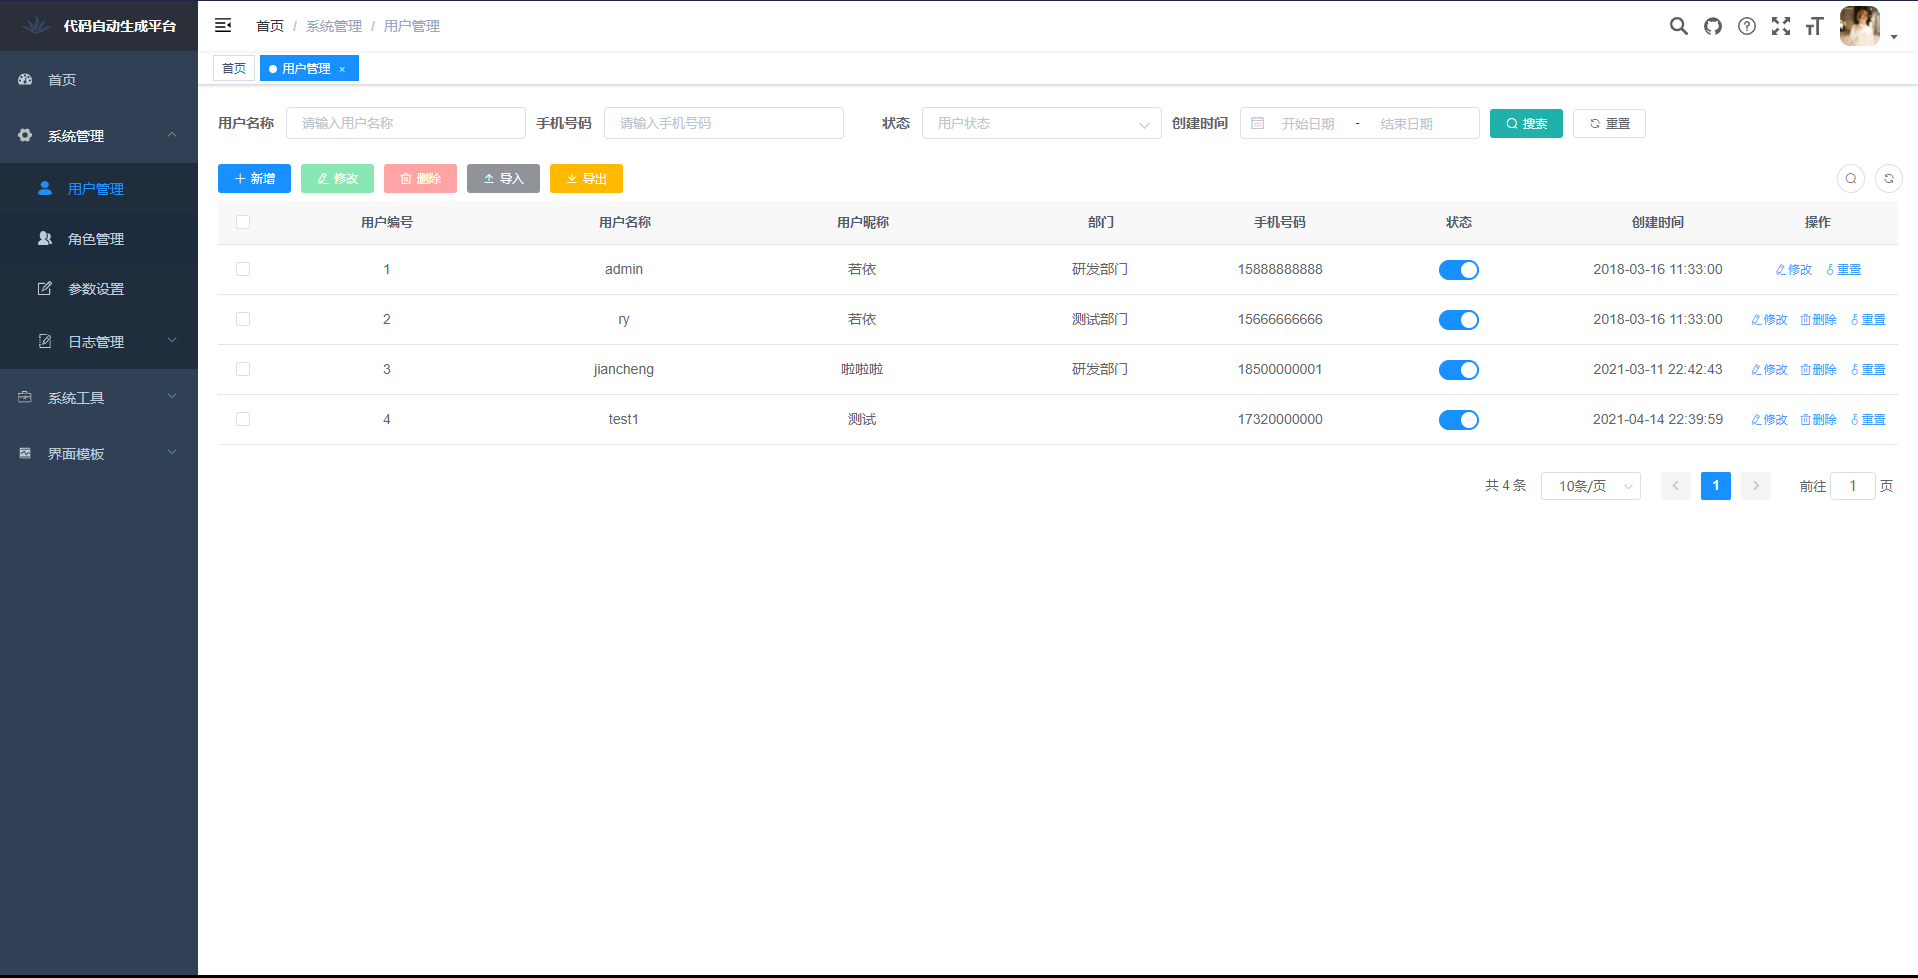
\includegraphics[width=0.95\textwidth]{figures/fig5-2.png}
  \caption{用户管理功能界面图}
  \label{fig5-2}
\end{figure}

管理员在新增或修改用户信息时可为用户分配角色，本系统角色包含管理员、普通用户。如图 \ref{fig5-3} 所示。

\begin{figure}[H]
  \centering
  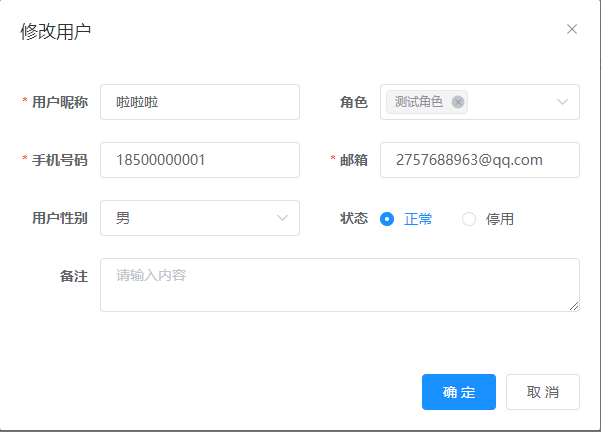
\includegraphics[width=0.55\textwidth]{figures/fig5-3.png}
  \caption{用户管理功能—修改用户信息}
  \label{fig5-3}
\end{figure}

\section{角色管理功能}
角色管理功能是基于本系统的配置用户角色权限的系统功能模块。本功能通过分页查询展示所有系统角色，管理员可通过角色名称、权限、角色状态等作为条件对所需角色进行查询。管理员能够通过滑块对列表中的角色进行启用或停用操作，停用的角色无法分配给用户。

在新增或修改角色时，能够为该角色分配权限，即该角色下用户能够使用哪些系统功能。该角色下的用户登录系统后将只能看到该角色具有的功能。管理员也可以根据具体需求自定义数据权限。

管理员在选择多个角色后，可通过列表顶部的操作按钮对选中数据进行批量删除和导出（Excel）等操作。当角色已被分配给系统用户后，将不允许删除。当没有选择角色信息时，点击导出按钮将默认导出全部角色的查询结果。如图 \ref{fig5-4} 所示。

\begin{figure}[H]
  \centering
  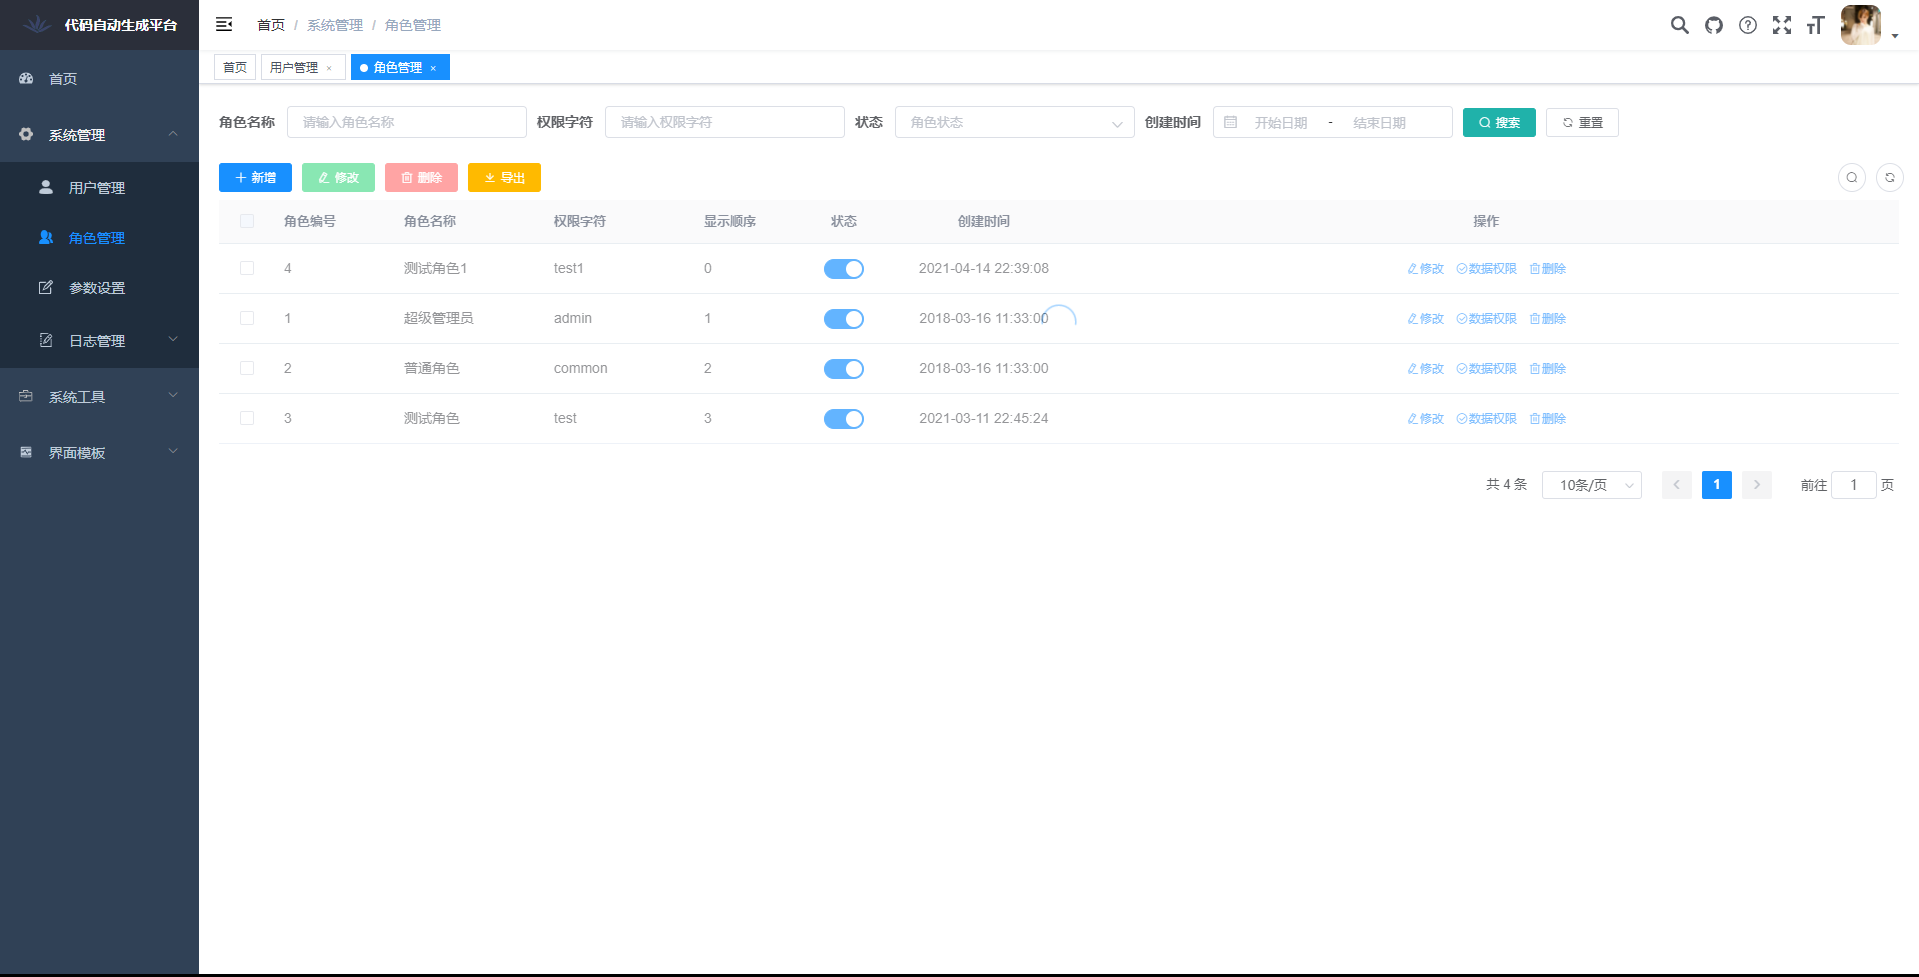
\includegraphics[width=0.95\textwidth]{figures/fig5-4.png}
  \caption{角色管理功能界面图}
  \label{fig5-4}
\end{figure}

\section{系统参数设置功能}
系统参数设置功能模块是本系统的一个方便于用户个性化设置的辅助系统功能模块。系统通过列表的形式展示全部参数设置信息，用户可通过参数名、参数字段、内容等作为条件对参数配置信息进行查询，列表中展示配置名、配置参数、配置效果等信息。用户可通过本功能实现对系统样式、初始化密码值、系统颜色、整体页面框架的动态配置。

用户选择多个配置信息后可对所选信息进行批量删除、导出操作（导出规则同用户管理功能和角色管理功能）。

用户在完成参数设置并提交后即可生效，若配置没有生效，可点击清理缓存按钮手动清理浏览器缓存，对参数配置完成更新。如图 \ref{fig5-5} 所示。

\begin{figure}[H]
  \centering
  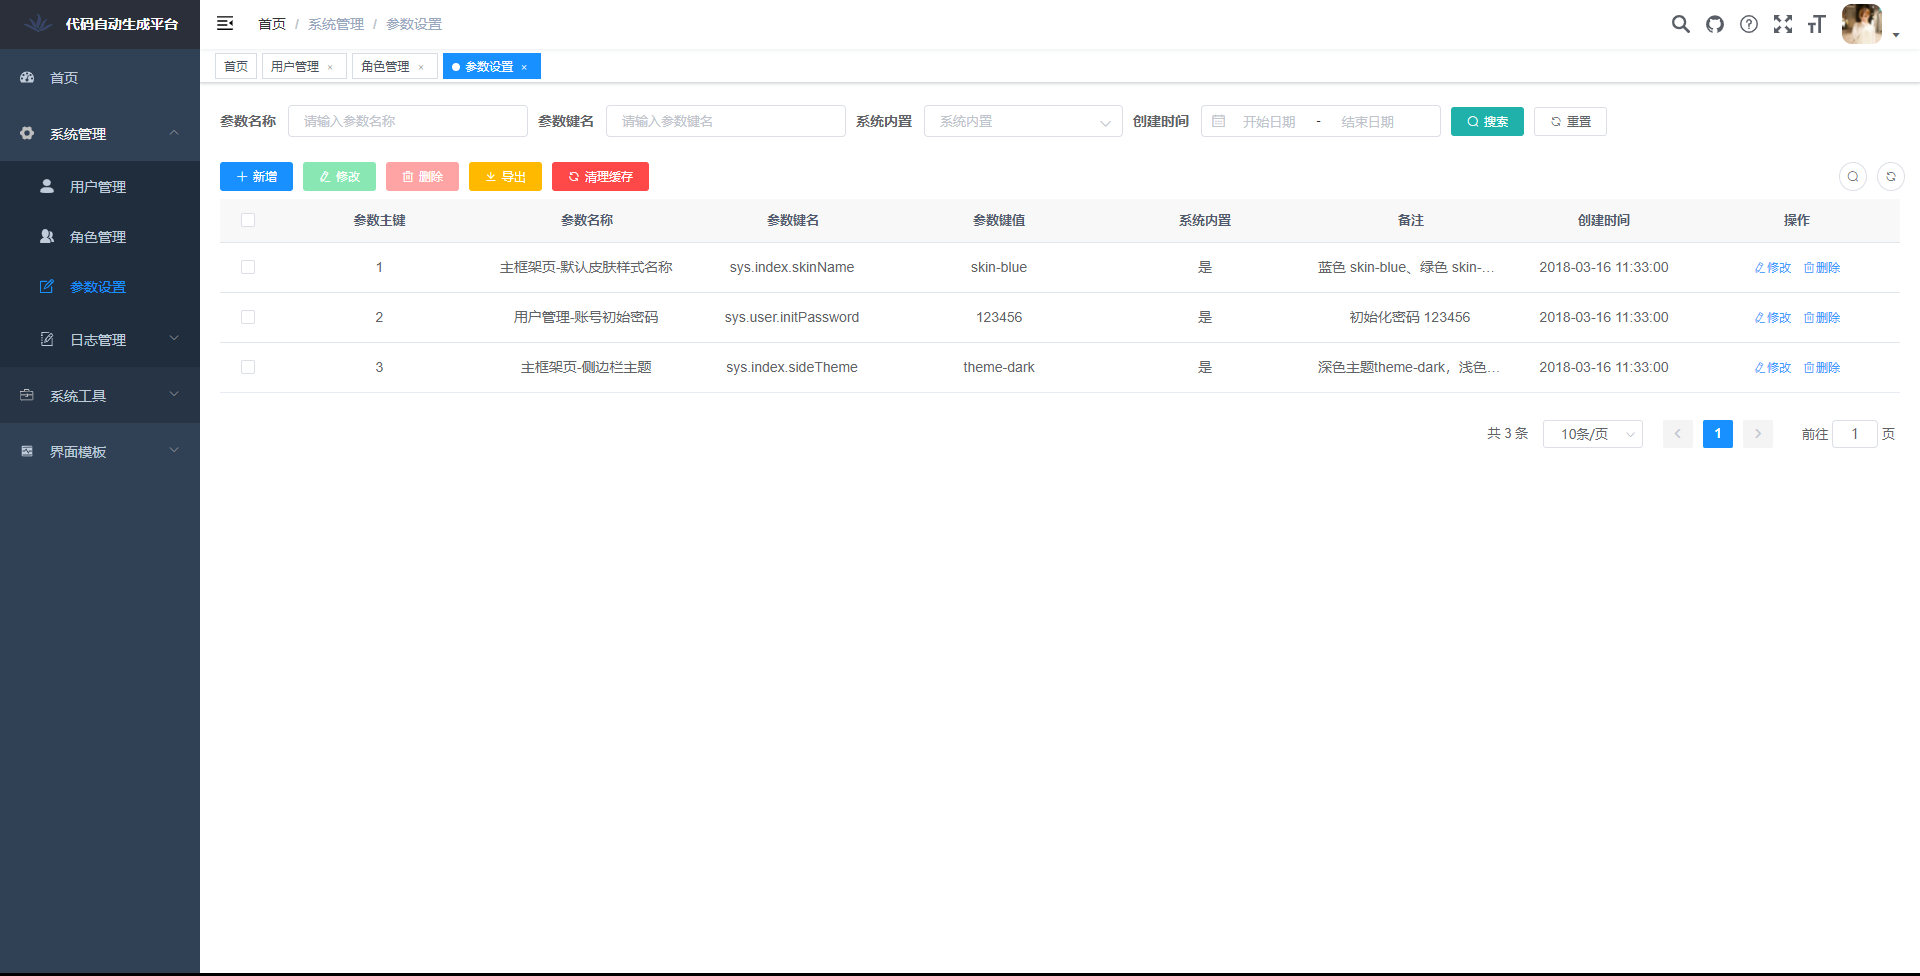
\includegraphics[width=0.95\textwidth]{figures/fig5-5.png}
  \caption{系统参数设置功能界面图}
  \label{fig5-5}
\end{figure}

用户在添加或修改配置时需要填写相应参数名，通过配置参数键值数据实现对系统的动态设置。在配置完成后，系统会读取用户设置的参数，通过键名匹配到相应位置，再根据键值完成相应设置。如图 \ref{fig5-6} 所示。

\begin{figure}[H]
  \centering
  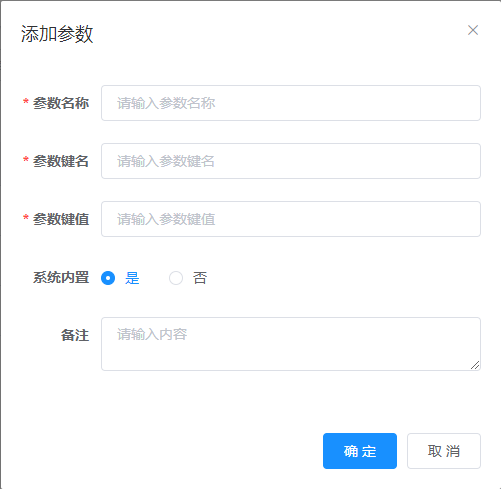
\includegraphics[width=0.5\textwidth]{figures/fig5-6.png}
  \caption{系统参数设置功能—新增或修改配置界面}
  \label{fig5-6}
\end{figure}

\section{系统日志功能}

\subsection{操作日志}
系统日志功能是基于本系统的辅助功能模块之一，对系统维护、错误排查有着重要作用。

用户在登录系统后进行的所有操作都会被记录下来，并在本功能中通过列表展示出来。管理员根据系统模块名、操作人、操作类型等条件对日志进行筛选。

管理员能对查询结果进行批量删除和导出（导出规则同上）。用户在导出数据后可通过清空功能，删除所有操作记录。如图 \ref{fig5-7} 所示。

\begin{figure}[H]
  \centering
  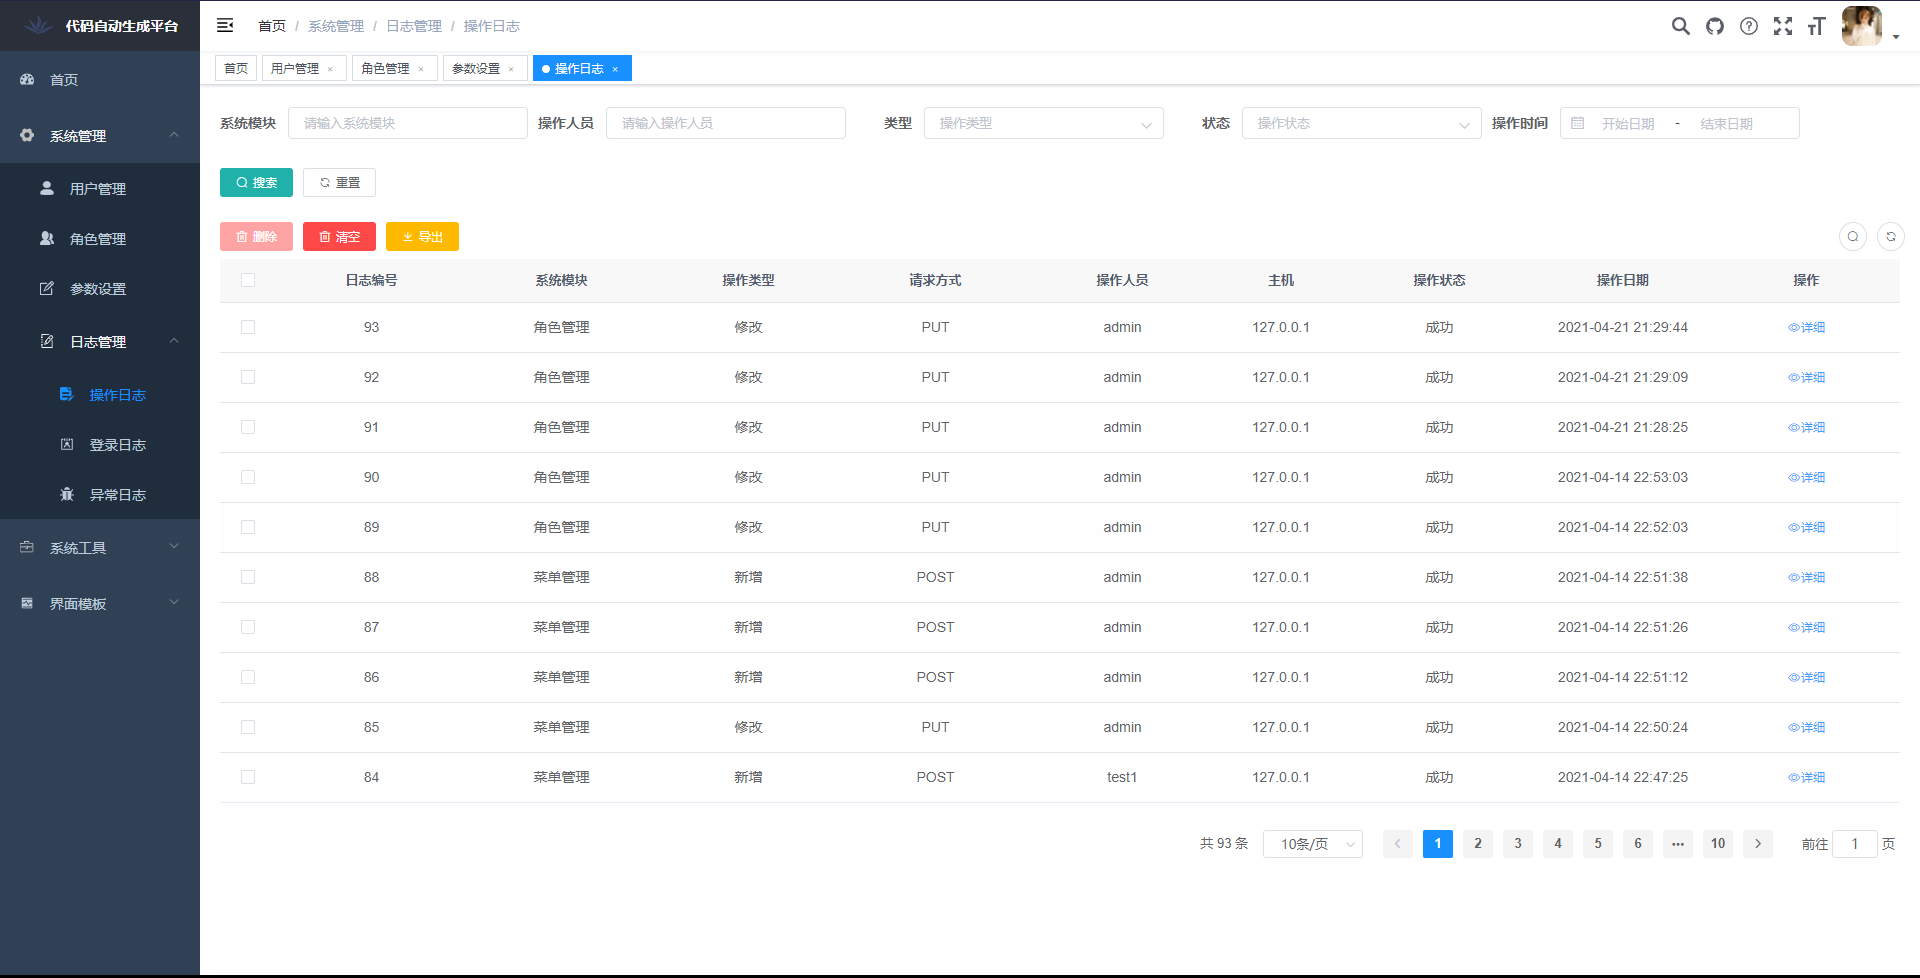
\includegraphics[width=0.95\textwidth]{figures/fig5-7.png}
  \caption{系统日志功能模块—操作日志界面图}
  \label{fig5-7}
\end{figure}

管理员点击列表中的详情按钮，可查看相应操作的详细信息，其中包括操作者、操作者 IP 地址、请求参数、请求方法名等。如图 \ref{fig5-8} 所示。

\begin{figure}[H]
  \centering
  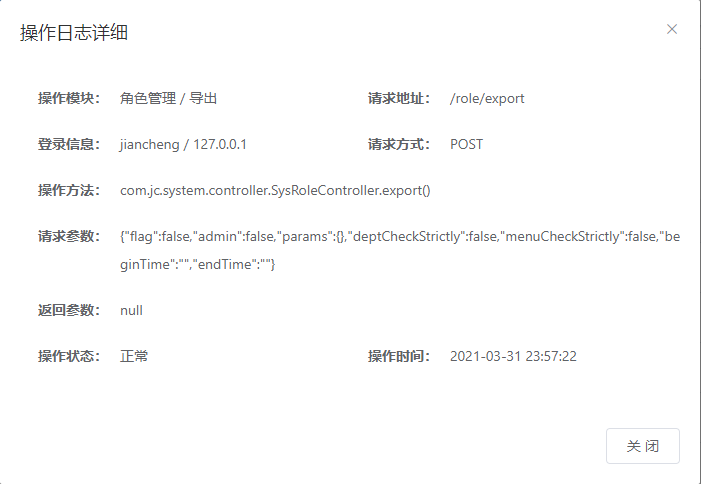
\includegraphics[width=0.6\textwidth]{figures/fig5-8.png}
  \caption{系统日志功能模块—操作日志—详情}
  \label{fig5-8}
\end{figure}

如下述代码所示，系统通过自定义注解实现实现对操作日志中操作模块名、操作功能（方法）、操作者和请求参数的获取，随后通过如下方式使用 @Log 注解传参的形式实现操作日志功能。

\begin{lstlisting}
@Target({ ElementType.PARAMETER, ElementType.METHOD })
@Retention(RetentionPolicy.RUNTIME)
@Documented
public @interface Log
{
    /**
     * 模块
     */
    public String title() default "";

    /**
     * 功能
     */
    public BusinessType businessType() default BusinessType.OTHER;

    /**
     * 操作人类别
     */
    public OperatorType operatorType() default OperatorType.MANAGE;

    /**
     * 是否保存请求的参数
     */
    public boolean isSaveRequestData() default true;
}
\end{lstlisting}

\subsection{登录日志}
登录日志是记录本系统所有用户（包括管理员）登录本系统时的信息，结合操作日志能更好的对系统进行维护。在系统遭到攻击时能通过系统日志对攻击者进行追踪。

当用户（管理员）登录系统时，系统通过 @Log 注解获取当前登录者的用户名、登录地址、登录状态等信息并存入数据控；在本功能中通过列表页的形式展示。

管理员通过登录地址、用户名等条件对登录信息进行条件查询。查询结果包括登录成功或失败、登录失败原因等信息，用户可对查询结果进行批量删除、清空和导出（导出规则同上）操作。如图 \ref{fig5-9} 所示。

\begin{figure}[H]
  \centering
  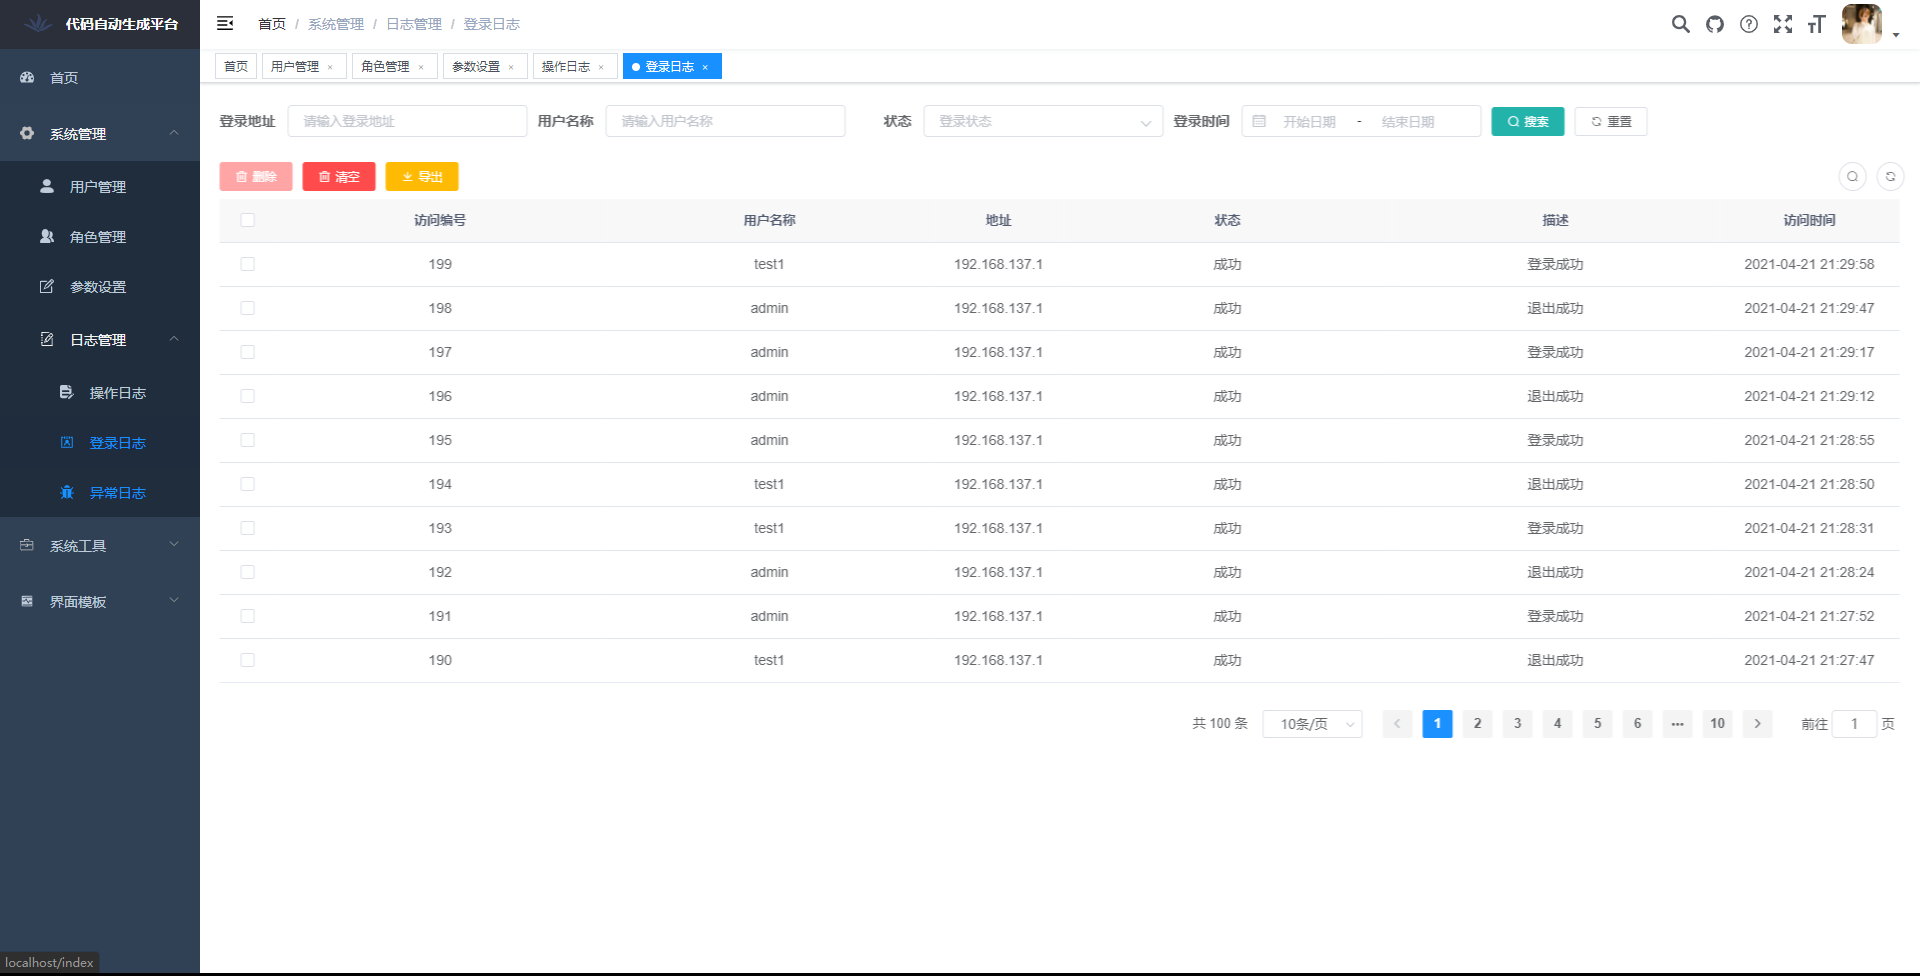
\includegraphics[width=0.95\textwidth]{figures/fig5-9.png}
  \caption{系统日志功能模块—登录日志界面图}
  \label{fig5-9}
\end{figure}

\section{页面构建功能}
页面构建功能是本系统的核心功能之一，用户通过拖拽或点击左侧组件栏中的组件，实现页面的个性化布局。

用户在选择组件后，组件将添加到中间的布局容器中，用户点击已选择的组件，可在右侧组件属性侧边栏中对该组件的属性进行设置。其中可设置生成后页面的绑定字段，组件栅格大小等，也可为表单组件添加校验规则。在右侧表单属性中能够设置当前表单名、表单模型名、表单校验模型名、表单栅格、表单尺寸等。

用户将鼠标划过或停留在已选择组件上时，显示复制和删除按钮，用户可对该组件进行复制或删除，复制的组件将具有完全相同的属性。用户不满意当前布局时可点击删除按钮删除该组件，或通过容器顶部的清空功能清空整个容器的内容。

在布局页面和运行页面都具有导出 Vue 文件和复制代码功能。用户在对当前页面完成构建后，可点击复制代码，随后选择生成页面或弹窗，系统将当前页面的代码复制到用户操作系统剪切板，最后用户可将代码直接粘贴到项目中。用户也可通过导出 Vue 文件功能，根据选择的表现形式将代码导出为 Vue 文件，然后可将该文件直接加入到项目制定目录中。如图 \ref{fig5-10} 所示。

\begin{figure}[H]
  \centering
  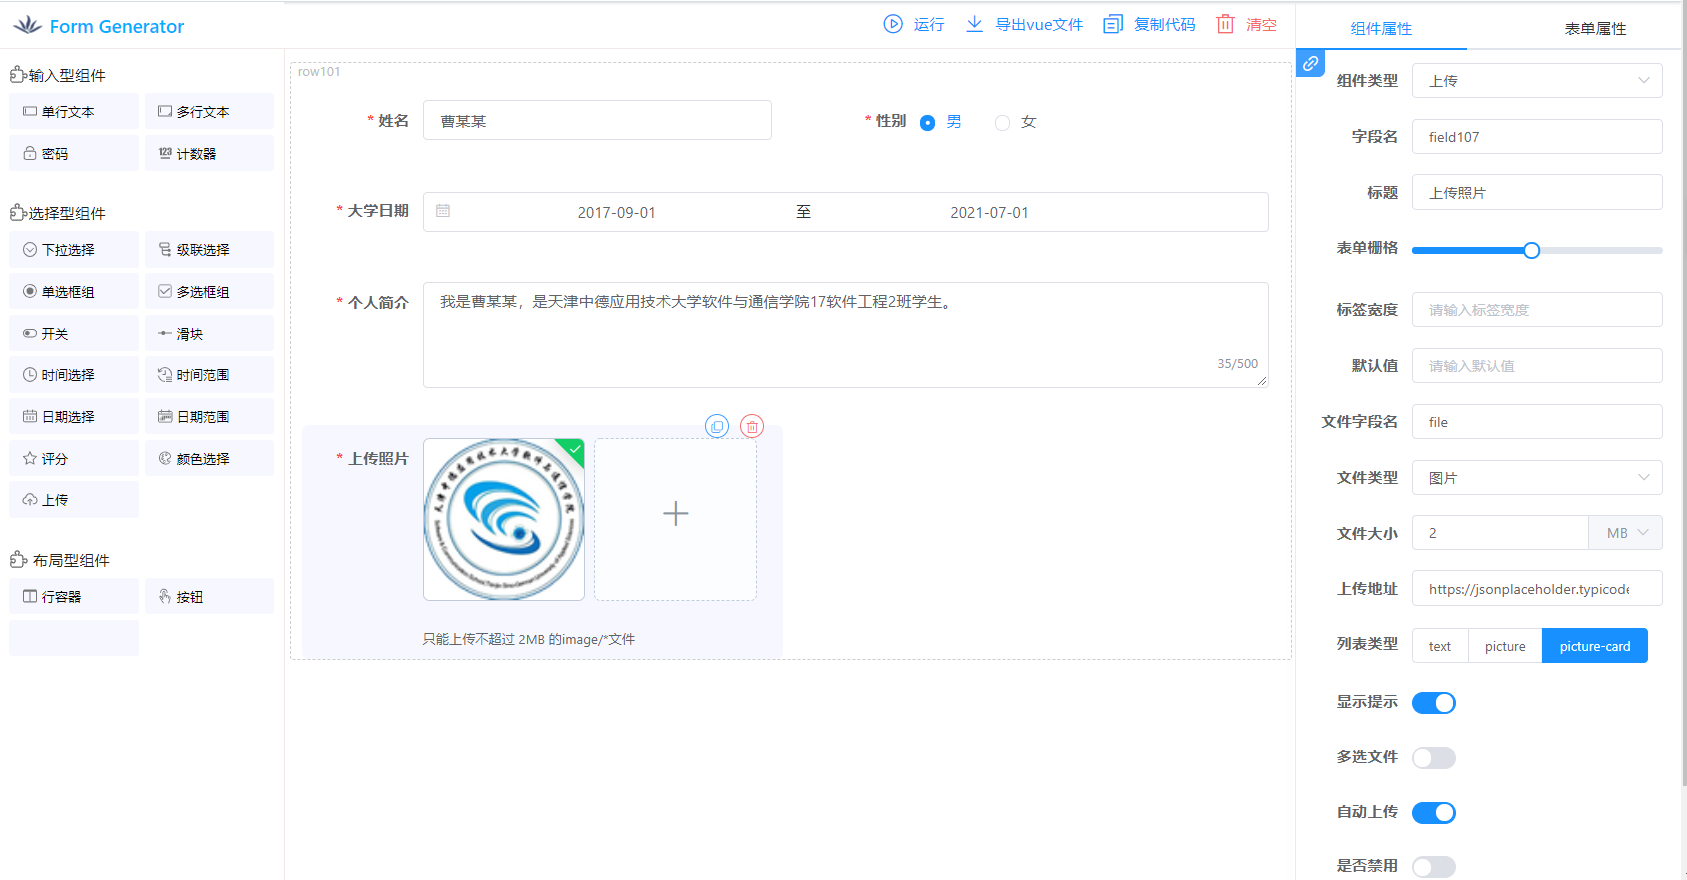
\includegraphics[width=0.95\textwidth]{figures/fig5-10.png}
  \caption{页面构建功能界面图}
  \label{fig5-10}
\end{figure}

如上述代码所示，通过 json 格式配置 ElementUI 中对应的组件，动态添加到页面左侧的组件库中。组件主要通过 document 属性后配置 ElementUI 官网组件地址动态拉取组件信息，通过对应前端标签属性中的 label、placeholder、clearable、format 等属性的配置，从而实现选择组件后默认标签样式的设置。

\begin{lstlisting}
{
  __config__: {
    label: '日期选择',
    tag: 'el-date-picker',
    tagIcon: 'date',
    defaultValue: null,
    showLabel: true,
    labelWidth: null,
    span: 24,
    layout: 'colFormItem',
    required: true,
    regList: [],
    changeTag: true,
    document: 'https://element.eleme.cn/#/zh-CN/component/date-picker'
  },
  placeholder: '请选择',
  type: 'date',
  style: { width: '100%' },
  disabled: false,
  clearable: true,
  format: 'yyyy-MM-dd',
  'value-format': 'yyyy-MM-dd',
  readonly: false
},
\end{lstlisting}

在加载页面时，系统根据 js 文件配置的组件属性在页面中生成相应的拖拽模块。前端页面通过 <draggable> 可移动段落标签和属性注入实现动态生成拖拽组件，随后通过自增 id 来区分相同组件。如下述代码所示。

\begin{lstlisting}
<draggable
    class="components-draggable"
    :list="inputComponents"
    :group="{ name: 'componentsGroup', pull: 'clone', put: false }"
    :clone="cloneComponent"
    draggable=".components-item"
    :sort="false"
    @end="onEnd"
>
    <div...>
</draggable>
\end{lstlisting}

当用户完成布局后，可通过运行功能在线编译当前页面。点击运行后选择生成弹窗或页面，然后可在左侧预览页面代码，在右侧查看当前页面；用户可通过右侧显示区对页面进行操作测试，并能够在左侧代码编辑区直接对页面代码进行修改。用户修改代码后点击刷新按钮重新编译，然后更新右侧页面显示效果。如图 \ref{fig5-11} 所示。

\begin{figure}[H]
  \centering
  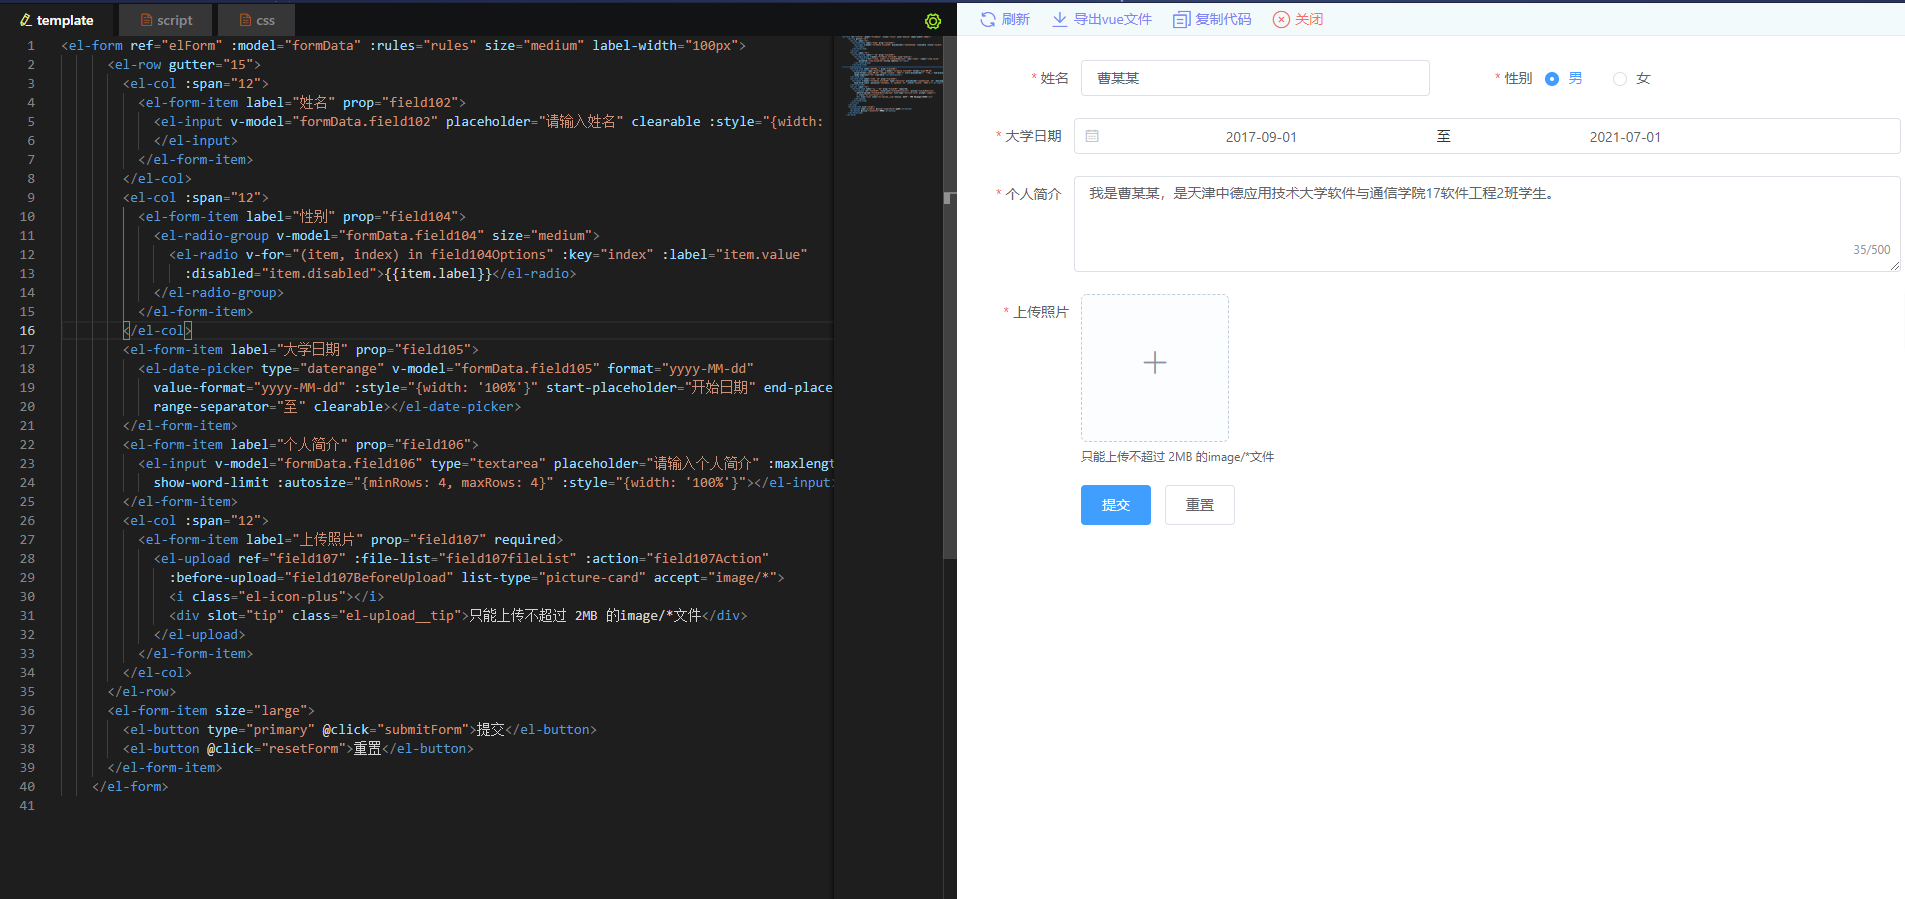
\includegraphics[width=0.95\textwidth]{figures/fig5-11.png}
  \caption{页面构建功能—运行（在线编译）}
  \label{fig5-11}
\end{figure}

在用户点击运行时会调用 makeUpHtml 方法，根据传入的表单配置和生成类型进行属性设置与过滤，然后将属性作为参数与 tags 对象中的组件名进行匹配，然后将属性动态赋值给相应的变量，完成代码生成。如下述代码所示。

\begin{lstlisting}
const tags = {
  'el-button': el => {
    const {
      tag, disabled
    } = attrBuilder(el)
    const type = el.type ? `type="${el.type}"` : ''
    const icon = el.icon ? `icon="${el.icon}"` : ''
    const round = el.round ? 'round' : ''
    const size = el.size ? `size="${el.size}"` : ''
    const plain = el.plain ? 'plain' : ''
    const circle = el.circle ? 'circle' : ''
    let child = buildElButtonChild(el)

    if (child) child = `\n${child}\n` // 换行
    return `<${tag} ${type} ${icon} ${round} ${size} ${plain}
            ${disabled} ${circle}>${child}</${tag}>`
  },
\end{lstlisting}

\section{代码生成功能}
代码生成功能是本系统的核心功能模块之一。用户在创建完数据表后点击导入按钮，在弹窗中查找并选择要导入的数据表，点击确定。如图 \ref{fig5-12} 所示。

\begin{figure}[H]
  \centering
  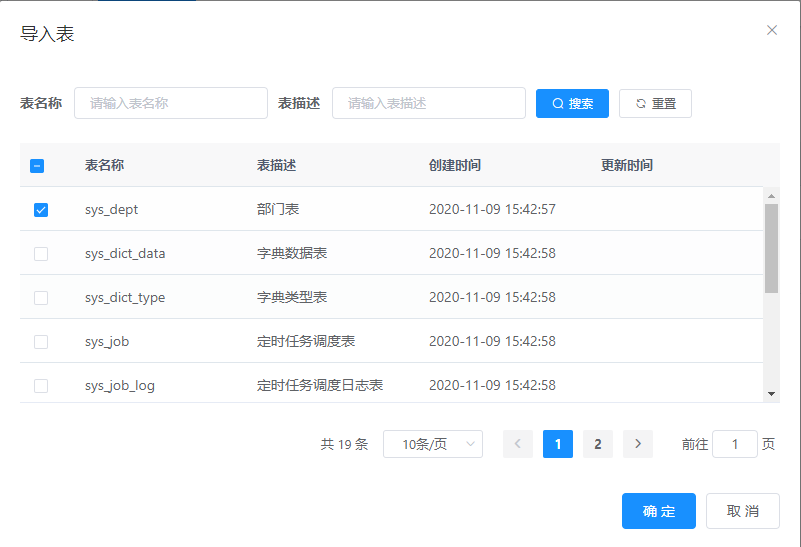
\includegraphics[width=0.7\textwidth]{figures/fig5-12.png}
  \caption{代码生成功能—导入数据表}
  \label{fig5-12}
\end{figure}

用户在导入数据表后，本功能列表页中将显示已导入的数据表信息。用户可通过表名等对数据表进行查询。当已导入数据表被修改，用户点击操作项中的同步按钮，可将已导入的数据表信息强制更新。用户能够通过选择已导入数据表信息进行批量删除或单独删除操作。

如下述代码所示，用户在点击生成按钮后，通过访问后端接口 batchGenCode 后进入处理部分；在这过程中，Java 使用了字节输出流、压缩包类，通过 generatorCode 方法查询生成代码的表信息并生成相应代码，完成后终止输出流，调用浏览器下载功能完成生成操作。

\begin{lstlisting}
/**
 * 生成代码（下载方式）
 *
 * @param tableName 表名称
 * @return 数据
 */
@Override
public byte[] downloadCode(String tableName) {
    ByteArrayOutputStream outputStream = new ByteArrayOutputStream();
    ZipOutputStream zip = new ZipOutputStream(outputStream);
    generatorCode(tableName, zip);
    IOUtils.closeQuietly(zip);
    return outputStream.toByteArray();
}
\end{lstlisting}

用户在完成对数据表的编辑后，可点击每一条数据后的生成代码按钮进行代码生成并下载；当用户需要对多个表进行生成时可勾选所需数据表的复选框，然后点击列表顶部的生成按钮实现多表生成代码并下载。如图 \ref{fig5-13} 所示。

\begin{figure}[H]
  \centering
  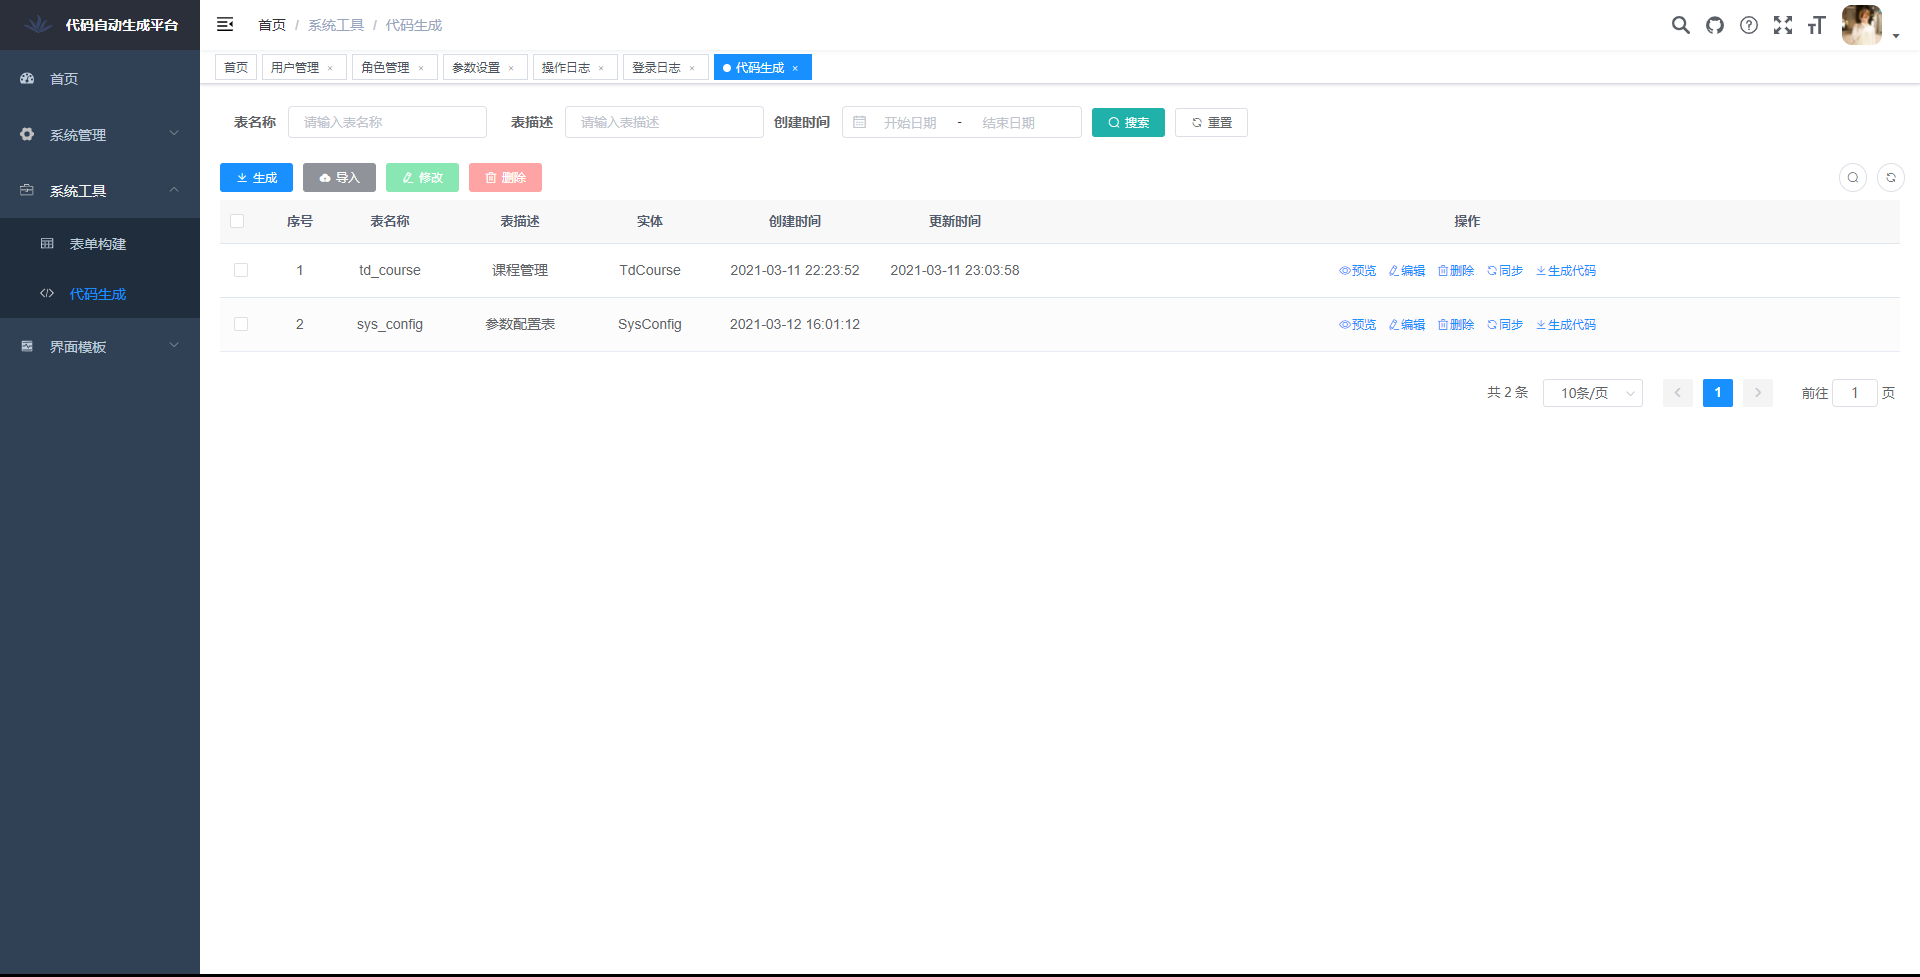
\includegraphics[width=0.95\textwidth]{figures/fig5-13.png}
  \caption{代码生成功能界面图}
  \label{fig5-13}
\end{figure}

用户点击操作项中的编辑按钮，可进入数据表信息编辑页面，该页面包括基本信息、字段信息、生成信息三个部分。

在基本信息中，用户可修改数据表名、数据表描述、生成 Java 代码的实体类名、作者等信息。如图 \ref{fig5-14} 所示。

\begin{figure}[H]
  \centering
  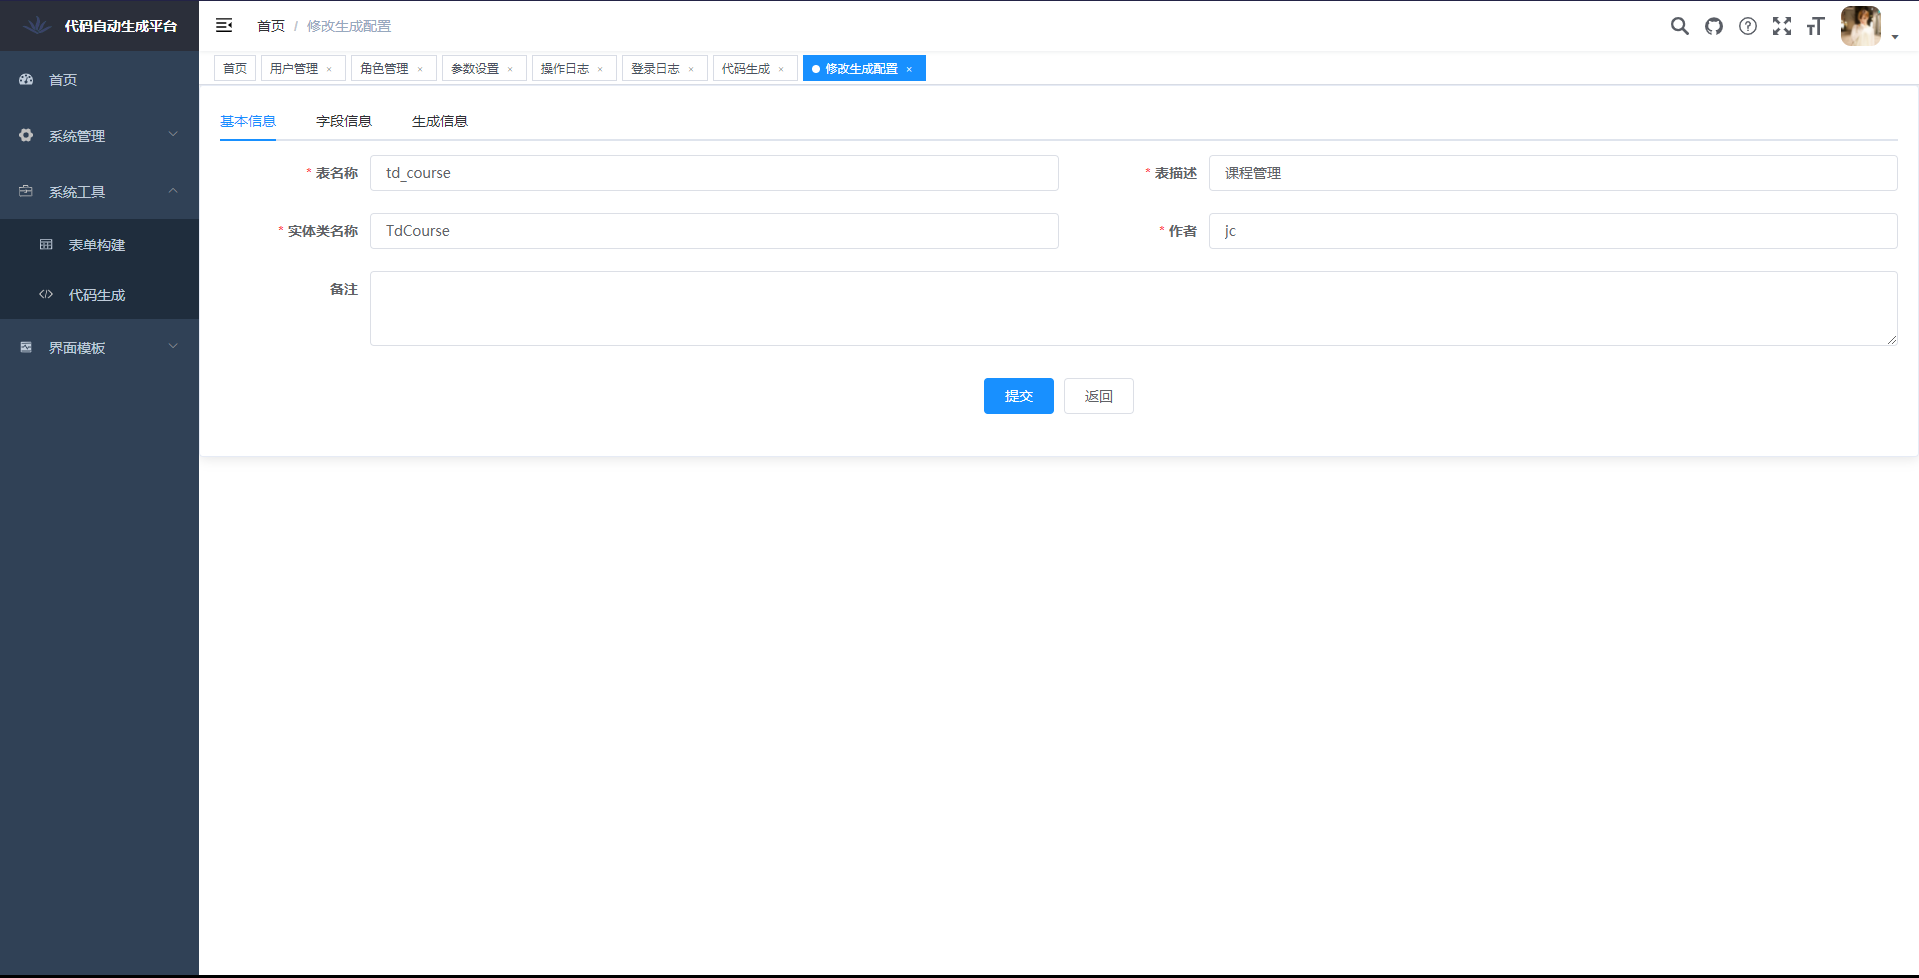
\includegraphics[width=0.95\textwidth]{figures/fig5-14.png}
  \caption{代码生成功能—编辑—基本信息}
  \label{fig5-14}
\end{figure}

用户在基本信息中首先能够编辑数据表字段的描述（备注），选择表字段对应的 Java 字段类型和属性名。然后选择该字段可进行的操作（插入、编辑、列表、查询），其次用户可选择该字段的查询方式，包括（不）等于、大于（等于）、小于（等于）、模糊查询、区间查询等几种类型。然后选择该字段是否为必填项，之后再选择该字段的显示类型，该类型有文本框（域）、下拉框、（单）复选框、日期、富文本编辑器等多种形式；在最后可为相应字段选择该字段对应的数据字典。如图 \ref{fig5-15} 所示。

\begin{figure}[H]
  \centering
  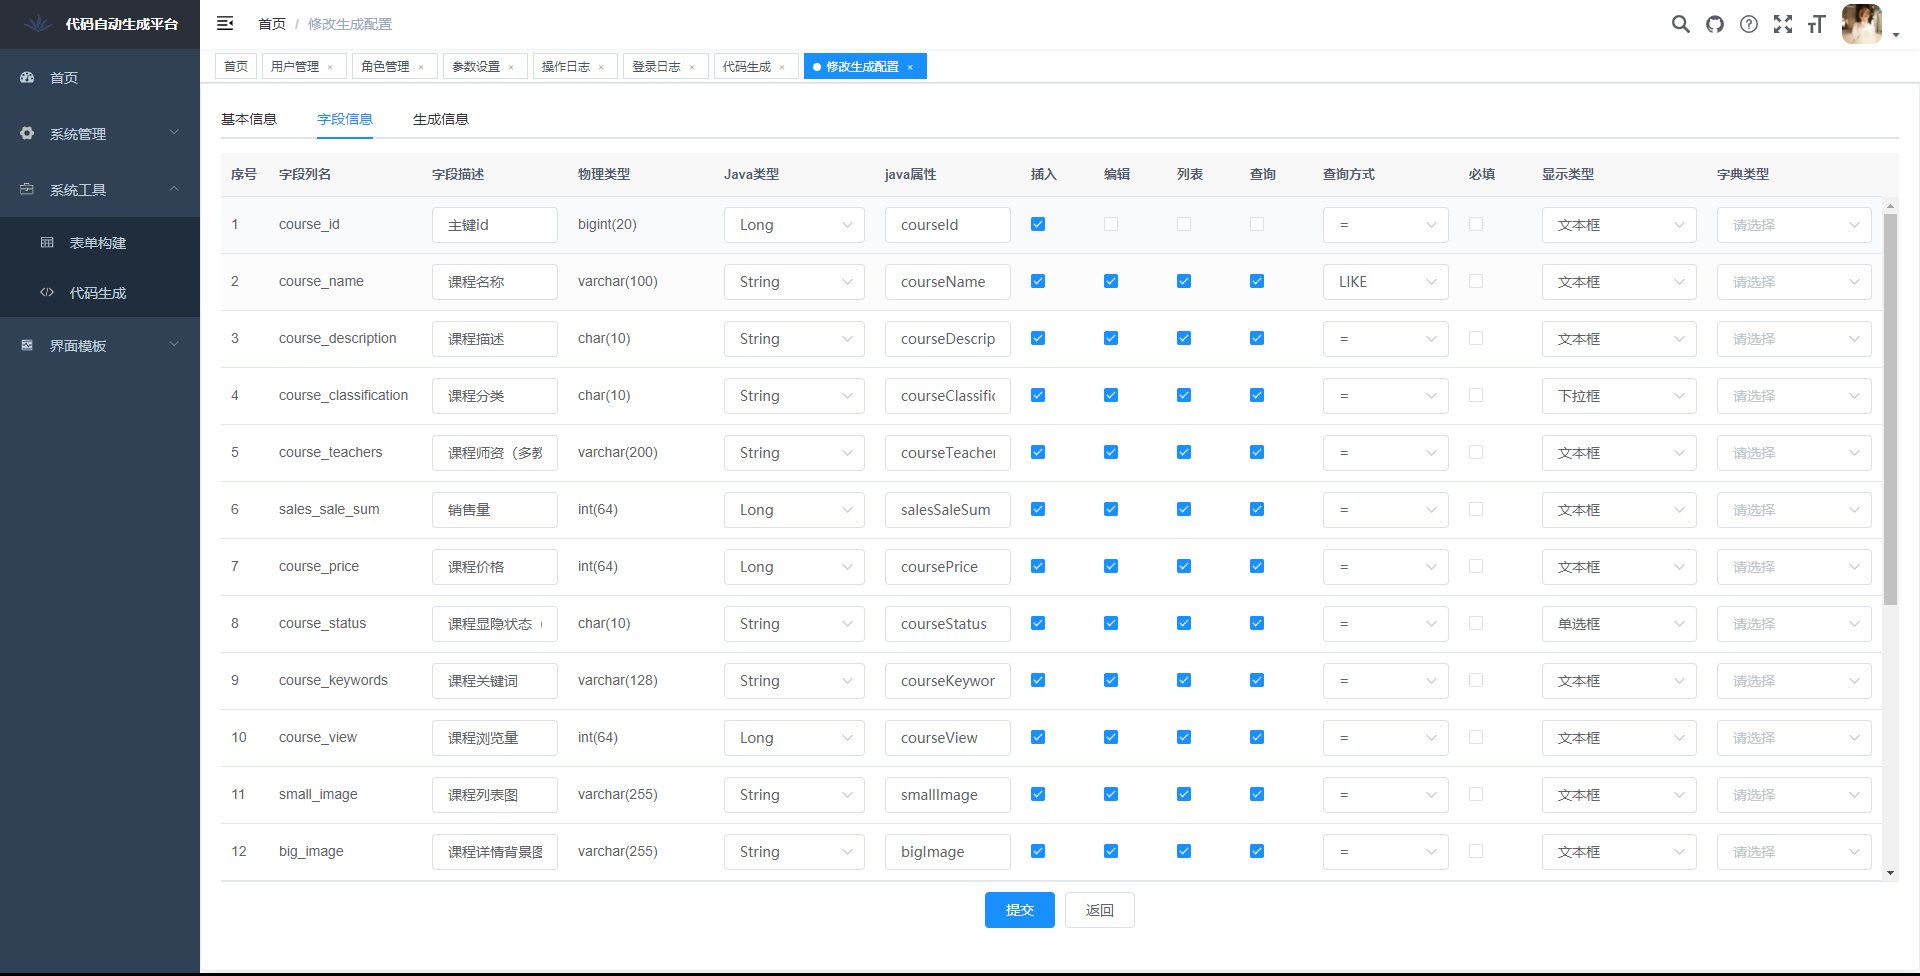
\includegraphics[width=0.95\textwidth]{figures/fig5-15.png}
  \caption{代码生成功能—编辑—字段信息}
  \label{fig5-15}
\end{figure}

在生成信息模块中用户可选择生成代码的数据模式（单表或树表），可根据实际项目编辑生成代码包的路径、生成的模块名、生成的业务名、生成的功能名。然后通过单选按钮，选择生成的代码形式；当用户选择 zip 压缩包时，生成代码文件为压缩包，当用户选择自定义路径时需填写生成路径名，在生成代码时本系统能根据该路径生成到相应目录下。

在树表模式下，用户可编辑树结构的关联字段和名称。如图 \ref{fig5-16} 所示。

\begin{figure}[H]
  \centering
  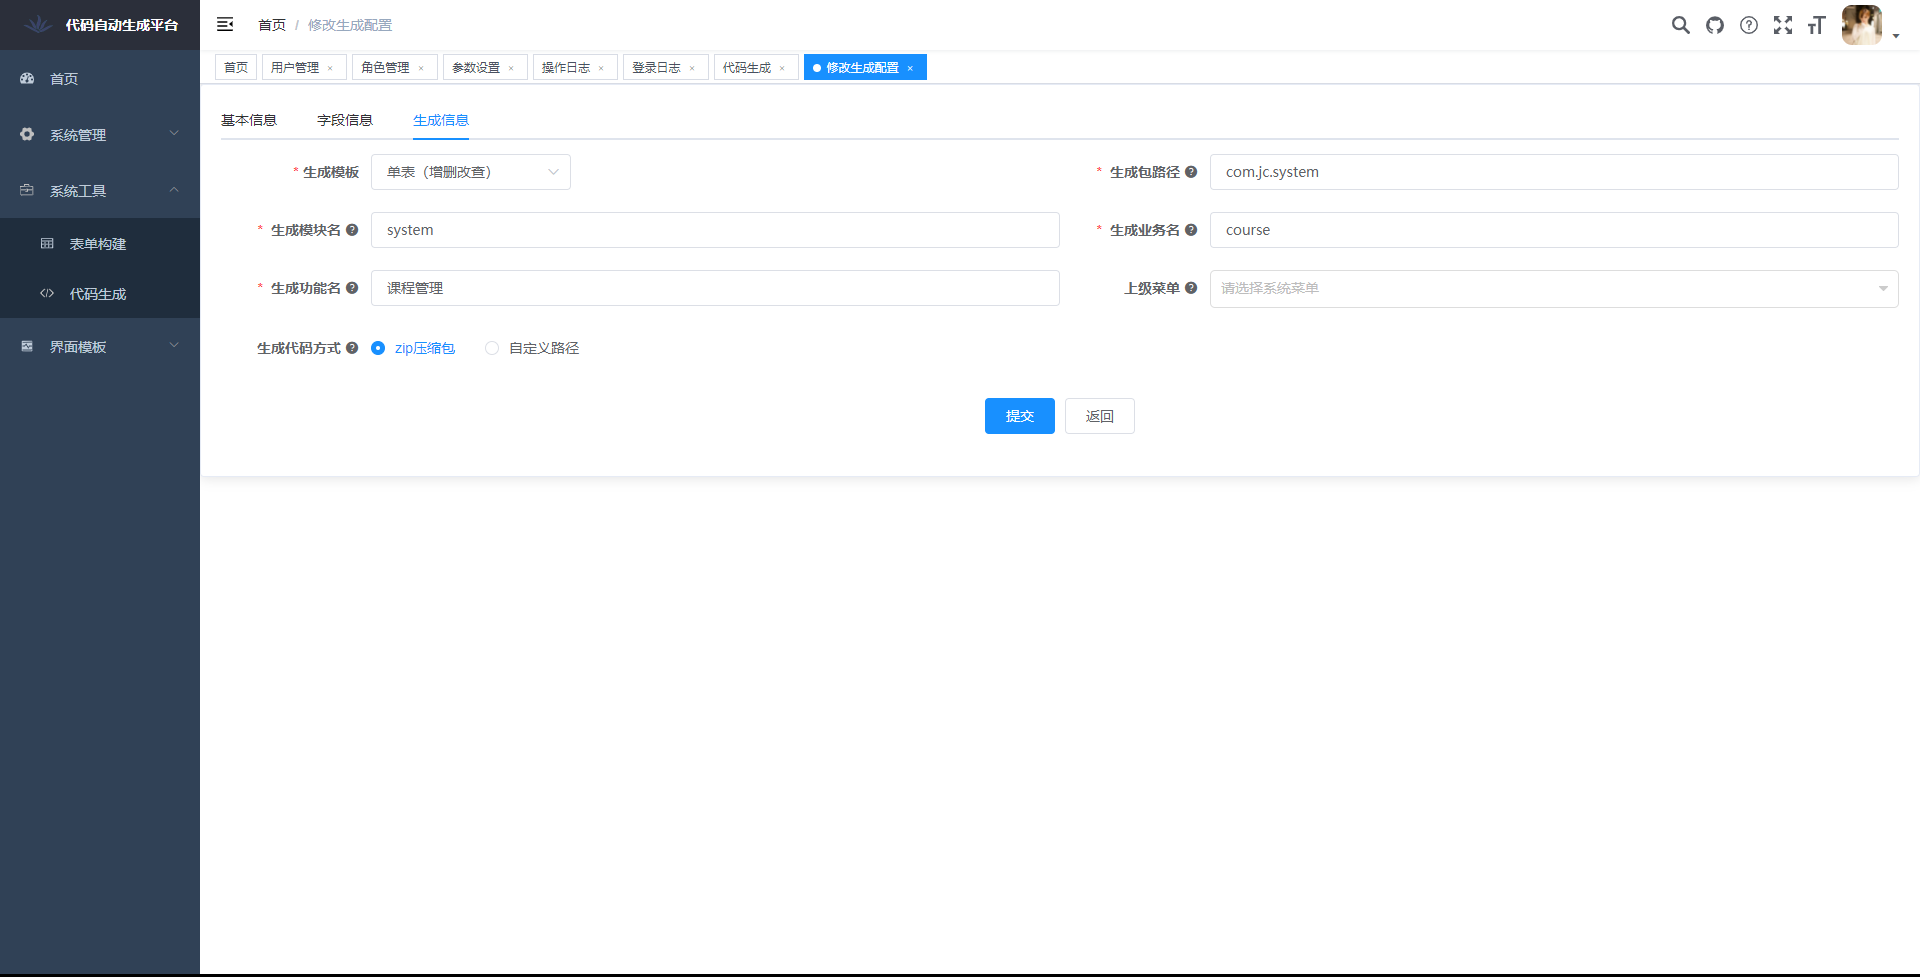
\includegraphics[width=0.95\textwidth]{figures/fig5-16.png}
  \caption{代码生成功能—编辑—生成信息}
  \label{fig5-16}
\end{figure}

用户在列表页点击预览按钮，系统将生成的代码通过弹窗的形式展示给用户，其中包含实体类、数据层、逻辑层、接口等 Java 代码，MyBatis 对应的 xml 文件，SQL 脚本文件，Vue 页面文件和 api 脚本文件。

如下述两段代码所示，后端在查询相应数据库表信息后通过输入流和 Velocity 生成类对代码模板进行渲染；前端根据后台返回的预览文件路径信息，按一定规则进行拼接后，直接读取指定代码文件，通过 <el-tab-pane> 和 <pre> 标签显示文件中代码内容。

\begin{lstlisting}
StringWriter sw = new StringWriter();
Template tpl = Velocity.getTemplate(template, Constants.UTF8);
tpl.merge(context, sw);
dataMap.put(template, sw.toString());
\end{lstlisting}

\begin{lstlisting}
<el-tabs v-model="preview.activeName">
  <el-tab-pane
    v-for="(value, key) in preview.data"
    :label="key.substring(key.lastIndexOf('/')+1,key.indexOf('.vm'))"
    :name="key.substring(key.lastIndexOf('/')+1,key.indexOf('.vm'))"
    :key="key"
  >
    <pre>{{ value }}</pre>
  </el-tab-pane>
</el-tabs>
\end{lstlisting}

当用户只需要某一两个页面代码时可在预览窗口中直接复制，免去下载等操作；同时，当用户在预览过程中发现代码中有需要调整的字段时，可及时返回编辑字段页面进行修改。如图 \ref{fig5-17} 所示。

\begin{figure}[H]
  \centering
  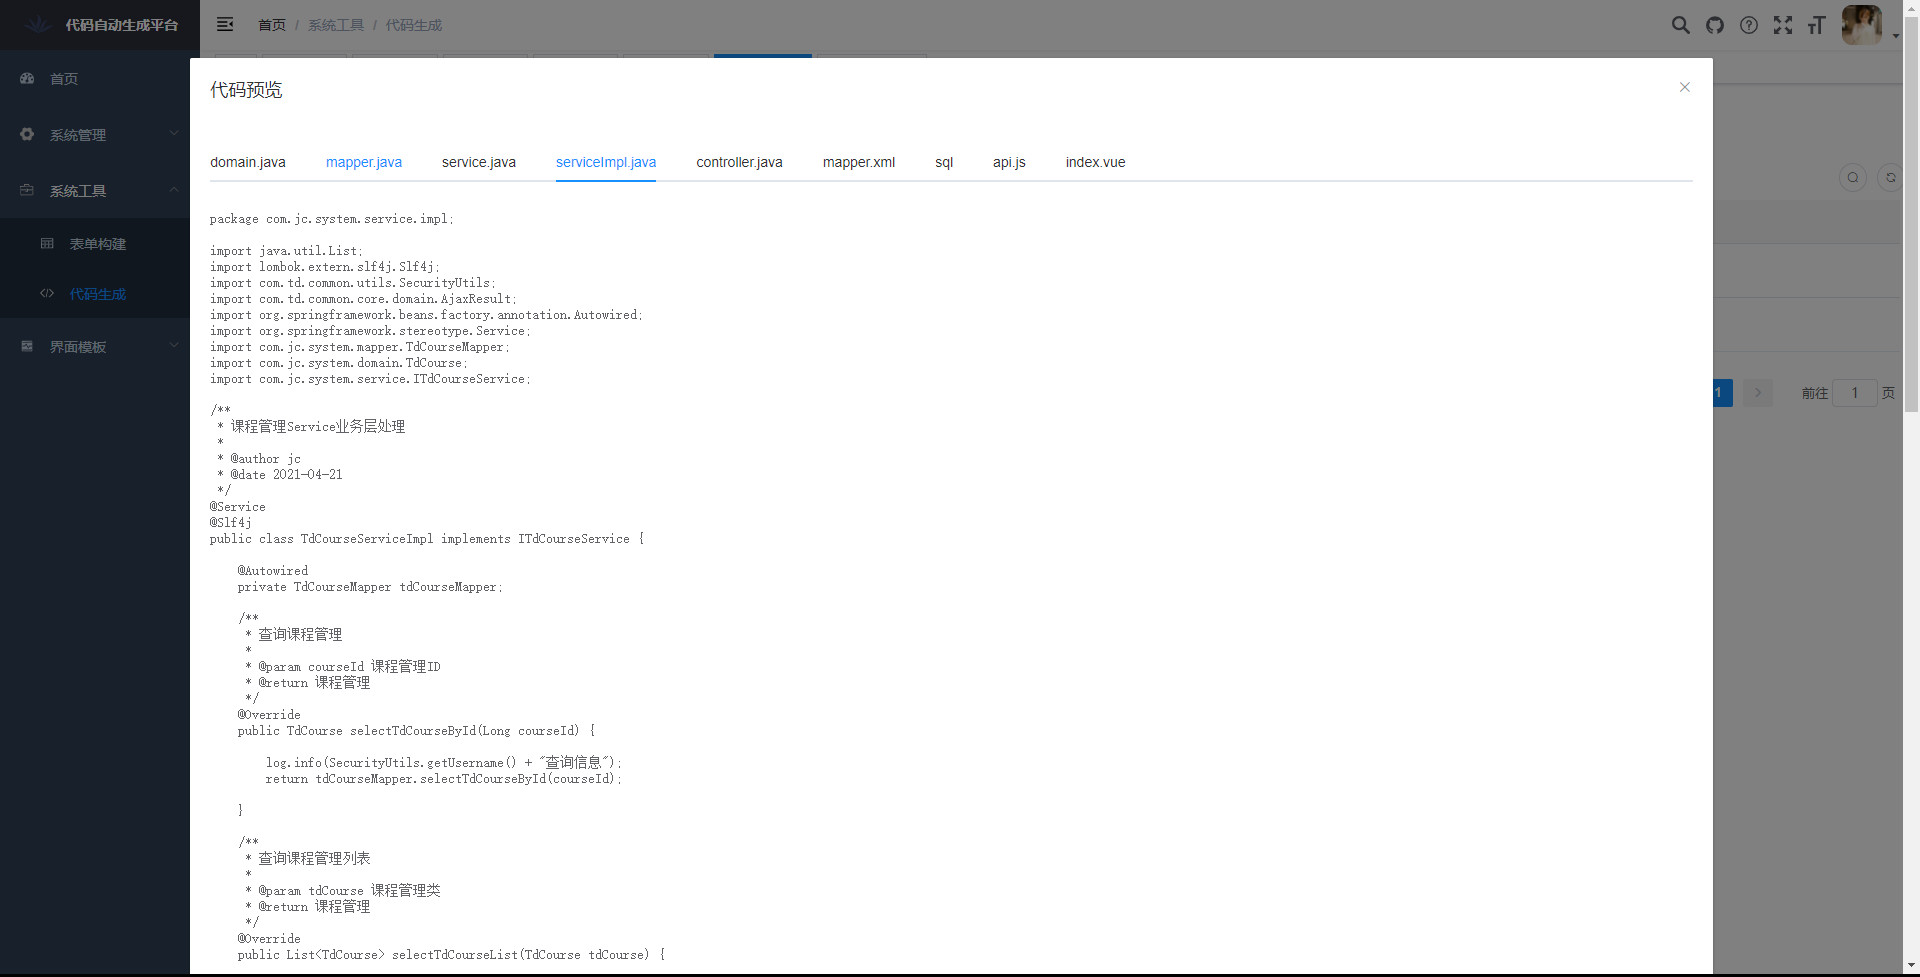
\includegraphics[width=0.95\textwidth]{figures/fig5-17.png}
  \caption{代码生成功能—预览}
  \label{fig5-17}
\end{figure}

\section{界面模板功能}
界面模板是本系统的特色功能。用户在构建页面后，可通过分享按钮将该模板文件分享到本功能中，之后其他用户可在本功能中看到其他用户分享的界面模板，并能进行查看或下载操作。如图 \ref{fig5-18} 所示。

\begin{figure}[H]
  \centering
  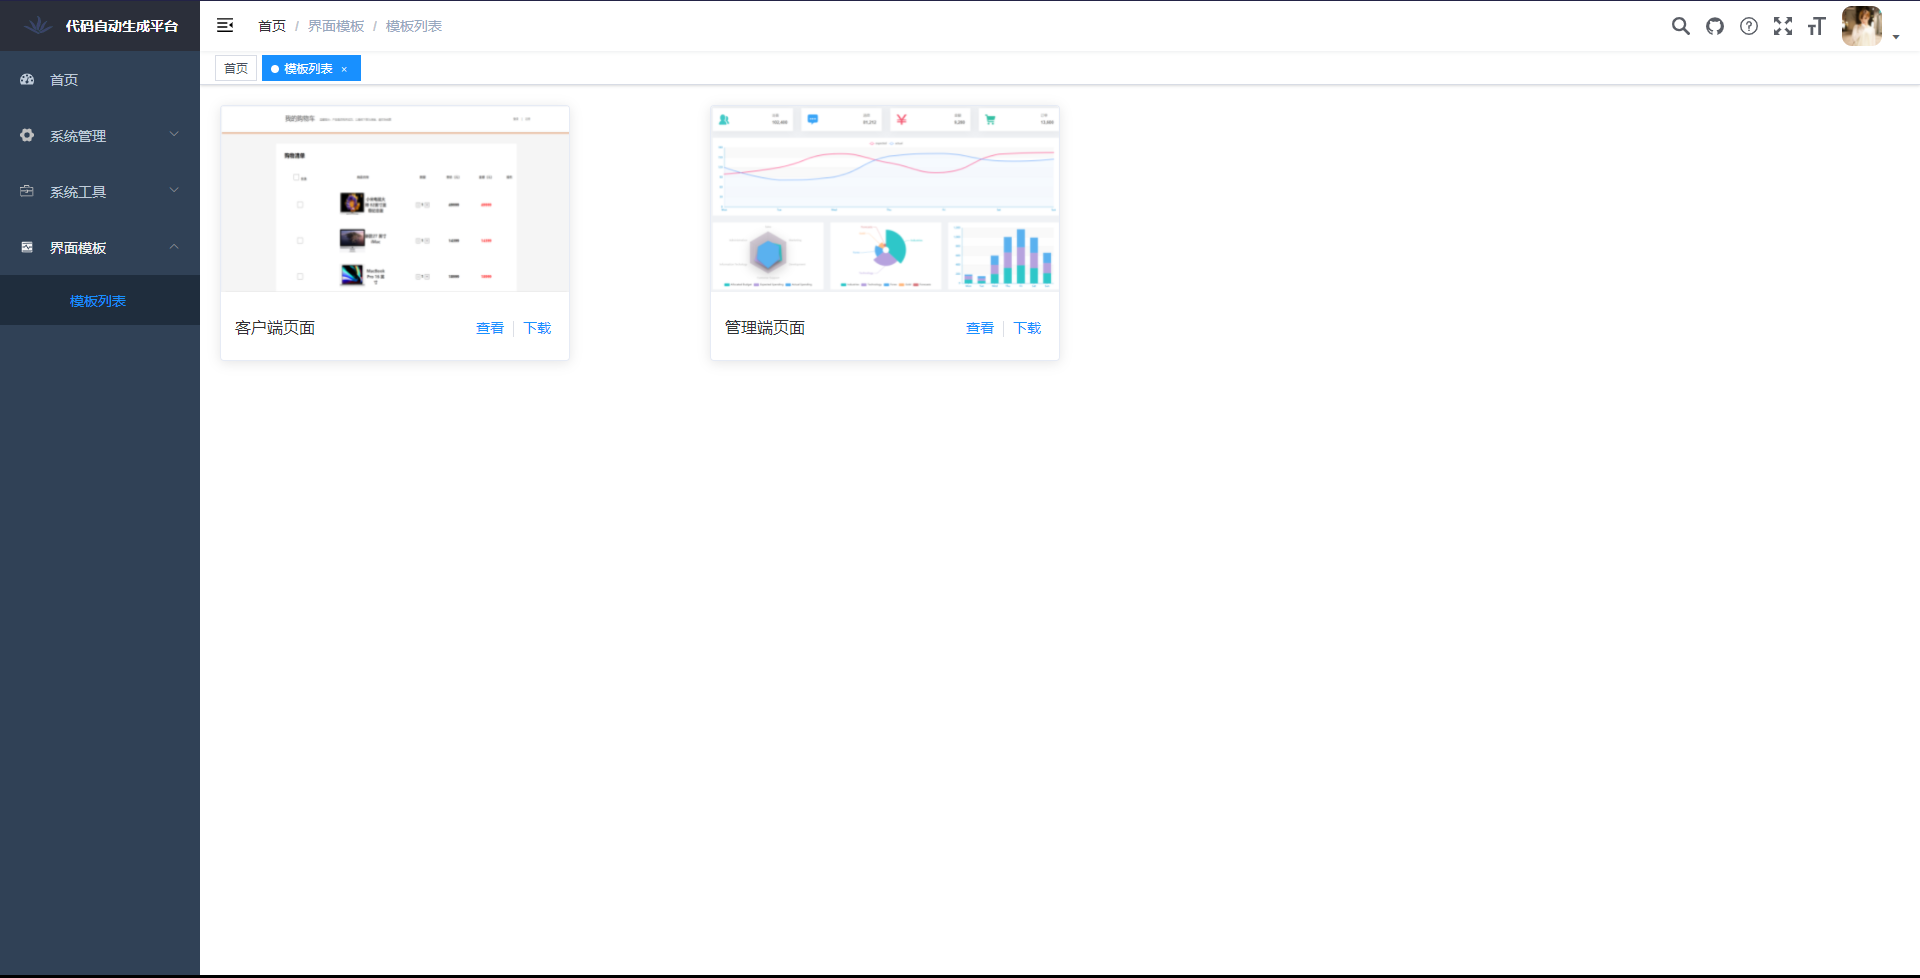
\includegraphics[width=0.95\textwidth]{figures/fig5-18.png}
  \caption{界面模板功能界面图}
  \label{fig5-18}
\end{figure}

如上述代码所示，根据后端返回的模板页的名称、文件路径、下载信息等数据，通过栅格化布局和 <el-card> 组件循环并排列展示，每一个页面都通过卡片的形式展示；当模板页过多时，通过懒加载的方式加载模板，这极大地改善了用户体验和对网络环境的依赖性。

\begin{lstlisting}
<el-col
    :span="5"
    v-for="(item, index) in dataList"
    :key="index" :offset="index > 0 ? 2 : 0"
>
  <el-card :body-style="{ padding: '0px' }">
    <img...>
    <div style="padding: 14px;">
      <span>{{ item.name }}</span>
      <div class="bottom clearfix" style="...">
        <el-button type="text" class="button" @click="look(item.path)">
          {{ item.look }}
        </el-button>
        <el-divider direction="vertical" />
        <el-button type="text" class="button" @click="down(item.path)">
          {{ item.down }}
        </el-button>
      </div>
    </div>
  </el-card>
</el-col>
\end{lstlisting}

用户点击查看按钮，系统根据该模板文件的 URL，将改模板文件嵌入到系统展示页中，然后用户可对该页面进行操作。图 \ref{fig5-19} 为通过页面构建功能生成的仿小米商城购物车页面。

\begin{figure}[H]
  \centering
  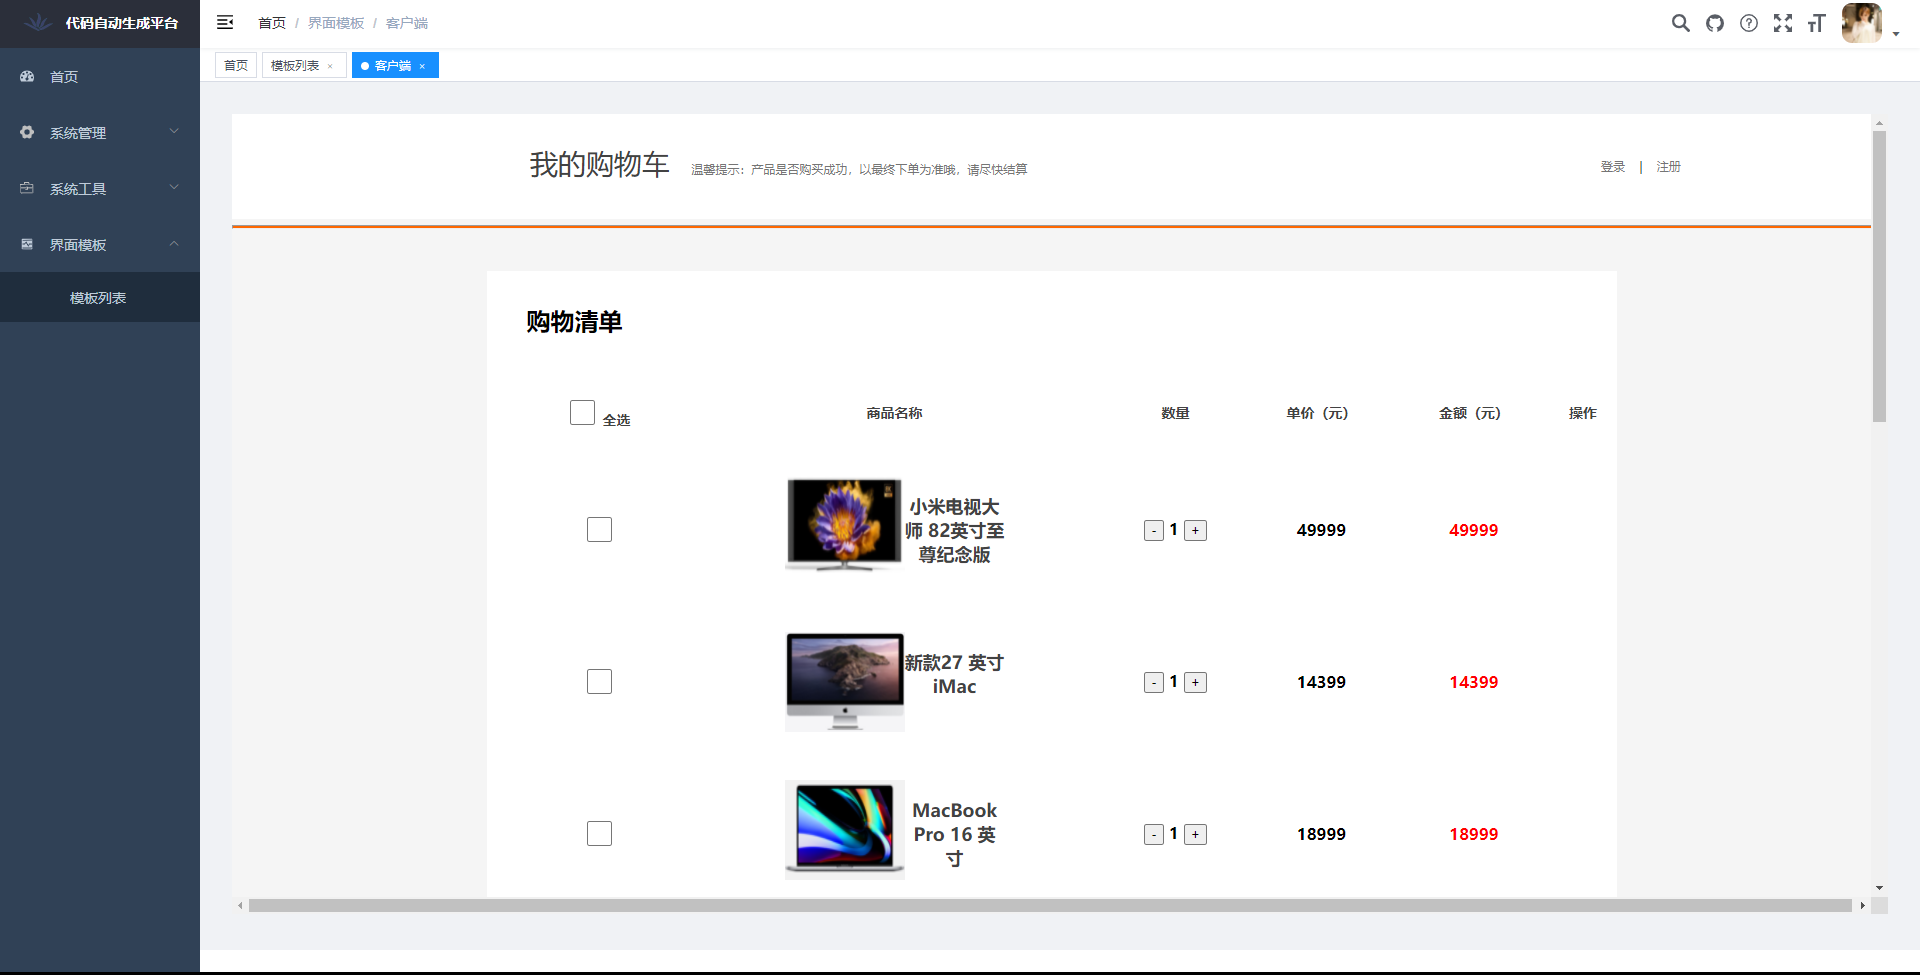
\includegraphics[width=0.95\textwidth]{figures/fig5-19.png}
  \caption{界面模板功能—查看模板}
  \label{fig5-19}
\end{figure}

\section{单元测试}
在平台开发完成后，根据平台功能编写相应的测试用例，根据测试用例对平台功能进行单元测试，检查平台的各项功能的结果是否符合预期。若结果与预期不符，记录产生问题原因和解决方案，随后编码完成对相应功能的修改。通过本次测试，共发现 3 处问题，随后及时记录并进行修改。如下表 \ref{tab5-1} 所示。

本平台使用阿里云 PTS 对整体系统进行压力和性能测试，随着并发量的增加，用户在查看界面模板和创建数据表时操作记录都会出现了死锁问题。最后通过给模板对象添加同步锁解决了大量用户同时访问模板资源造成的死锁问题；在创建数据表后进行记录时不再使用触发器，而是在数据表创建成功后再执行插入语句对创建记录进行插入，从而降低数据库发生死锁的可能性。

{\zihao{5}\songti
\begin{longtable}{c p{2.6cm} p{3.6cm} c p{4.2cm}}
    \caption{单元测试表}\label{tab5-1}\\
    \toprule
    序号 & 功能名 & 测试用例 & 是否成功 & 修正内容 \\
    \midrule
    \endfirsthead
    \toprule
    序号 & 功能名 & 测试用例 & 是否成功 & 修正内容 \\
    \midrule
    \endhead
    \bottomrule
    \endlastfoot
    1 & 用户管理功能 & 对系统用户进行增删改查操作 & 是 & / \\
    2 & 角色管理功能 & 对系统角色进行增删改查操作 & 是 & / \\
    3 & 系统参数设置功能 & 设置系统颜色参数为蓝色 & 否 & 原因：因系统无法获取前端传回的参数数据导致设置没有生效\newline 解决：给传回后台的参数属性添加映射 \\
    4 & 系统日志功能 & 登录系统，点击删除测试用户按钮后查看系统日志 & 是 & / \\
    5 & 上传下载功能 & 点击用户头像上传头像图片，点击下载按钮实现数据下载 & 是 & / \\
    6 & 创建数据表功能 & 点击“创建”按钮，填写数据表信息后点击提交完成创建 & 否 & 原因：因 MyBatis 中的语句书写不规范导表的创建报错\newline 解决：在 create 语句前后加入 <![CDATA[…]]> \\
    7 & 编辑生成配置功能 & 点击“修改”按钮后修改生成配置信息，点击提交完成修改 & 是 & / \\
    8 & 代码预览功能 & 点击“预览”按钮后，系统弹出相应代码的预览窗口 & 是 & / \\
    9 & 数据同步功能 & 点击“同步”按钮，再次打开相应数据表，表信息完成更新 & 是 & / \\
    10 & 组件拖拽功能 & 鼠标左键点击组件并按住，移动鼠标，组件随鼠标指针移动 & 是 & / \\
    11 & 代码生成功能 & 点击“生成”按钮，浏览器下载相应代码文件 & 是 & / \\
    12 & 组件属性编辑功能 & 改变组件属性，对应组件发生相应变化 & 是 & / \\
    13 & 页面属性编辑功能 & 改变页面属性，页面相应部分发生变化 & 是 & / \\
    14 & 在线预览功能 & 点击“运行”功能，打开组件界面预览页面 & 是 & / \\
    15 & 界面模板功能 & 点击“分享”按钮，相应模板在模板列表页显示 & 否 & 原因：因原文件上传路径为 Linux 系统路径，导致点击分享时无法找到路径，从而报错，模板列表也因此无法读取文件\newline 解决：将界面模板的存储路径修改为本机系统（Windows）的路径 \\
\end{longtable}}

\chapter{总结与展望}

\section{总结}
本文通过调查当前企业主流应用系统技术和客户主要需求，并在阅读、参考部分国内外相关文献的基础上，设计并实现了基于 SpringCloud 的企业系统自动生成平台。

首先，本文分析了当前国内外使用的几种主流代码生成技术，并基于方便用户使用等原则进行研究，比较得出当前代码生成平台在使用中的问题，针对这些问题进行需求分析。在考虑系统独立性、可扩展性等问题后，确定系统总体架构，再根据架构的设计思路完成本平台的数据库设计。根据系统需求分析结果，完成对系统功能的划分和详细设计，再此过程中对系统的主要功能进行阐述。

最终本平台能够为用户提供一个使用便捷、运行高效的代码生成平台，从创建数据表到最终生成代码，全部依托于本平台进行，用户甚至不需要具有编程能力。

本平台充分利用 SpringCloud 微服务架构特性，具有良好的扩展性和容错性，在一定程度上保障了良好的用户体验。得益于 SpringCloud 架构优点的同时，本平台也具有微服务架构的弊端。最直接体现在服务过多，部署、维护成本高，需要将每一个服务单独部署，尤其是系统整体迭代较快时，系统运维会占用大量时间。其次分布式系统开发的成本高，考虑容错性、分布式事务等方面，对开发者具有一定的挑战。

\section{展望}
得益于 SpringCloud 微服务架构的可扩展性和容错性，在今后开发中，本平台将作为一个高可用系统服务于各类用户。开发者可以以本平台为基础，进行个性化开发，将个性化需求注册为服务并集成到本系统中，直接在指定目录下生成代码，进一步简化开发过程。

其次本平台将逐步加入运维监控功能，实时监控平台的运行环境，出现内存不足等问题提前报警，进一步提高平台的可用性。

\izdbibliography{ref}

\begin{acknowledgements}
我能够顺利完成毕业设计，首先要感谢我的指导老师——张磊老师。张磊老师悉心指导我论文的每一部分内容，为我讲解论文的编写规范，每一版论文老师都会认真检查并给出许多修改意见。张磊老师在辅导我论文的基础上，还为我毕业设计的研究方向给出了指导性意见，在实现设计的过程中引导我解决困难。同时张磊老师作为我的班主任，从大二开始培养我的开发能力，不断提高我的技术水平和开发思想，为我的毕业设计的实现打下了坚实基础。

感谢我的父母一直以来对我的支持，是他们的辛勤付出给了我一个安心学习的环境，他们对我的鼓励和关怀是我不断进步的动力。

最后，感谢各位老师在百忙之中抽出时间参加论文答辩会。
\end{acknowledgements}

\end{document}
